% Options for packages loaded elsewhere
\PassOptionsToPackage{unicode}{hyperref}
\PassOptionsToPackage{hyphens}{url}
%
\documentclass[
]{book}
\usepackage{amsmath,amssymb}
\usepackage{lmodern}
\usepackage{iftex}
\ifPDFTeX
  \usepackage[T1]{fontenc}
  \usepackage[utf8]{inputenc}
  \usepackage{textcomp} % provide euro and other symbols
\else % if luatex or xetex
  \usepackage{unicode-math}
  \defaultfontfeatures{Scale=MatchLowercase}
  \defaultfontfeatures[\rmfamily]{Ligatures=TeX,Scale=1}
\fi
% Use upquote if available, for straight quotes in verbatim environments
\IfFileExists{upquote.sty}{\usepackage{upquote}}{}
\IfFileExists{microtype.sty}{% use microtype if available
  \usepackage[]{microtype}
  \UseMicrotypeSet[protrusion]{basicmath} % disable protrusion for tt fonts
}{}
\makeatletter
\@ifundefined{KOMAClassName}{% if non-KOMA class
  \IfFileExists{parskip.sty}{%
    \usepackage{parskip}
  }{% else
    \setlength{\parindent}{0pt}
    \setlength{\parskip}{6pt plus 2pt minus 1pt}}
}{% if KOMA class
  \KOMAoptions{parskip=half}}
\makeatother
\usepackage{xcolor}
\usepackage{color}
\usepackage{fancyvrb}
\newcommand{\VerbBar}{|}
\newcommand{\VERB}{\Verb[commandchars=\\\{\}]}
\DefineVerbatimEnvironment{Highlighting}{Verbatim}{commandchars=\\\{\}}
% Add ',fontsize=\small' for more characters per line
\usepackage{framed}
\definecolor{shadecolor}{RGB}{248,248,248}
\newenvironment{Shaded}{\begin{snugshade}}{\end{snugshade}}
\newcommand{\AlertTok}[1]{\textcolor[rgb]{0.94,0.16,0.16}{#1}}
\newcommand{\AnnotationTok}[1]{\textcolor[rgb]{0.56,0.35,0.01}{\textbf{\textit{#1}}}}
\newcommand{\AttributeTok}[1]{\textcolor[rgb]{0.77,0.63,0.00}{#1}}
\newcommand{\BaseNTok}[1]{\textcolor[rgb]{0.00,0.00,0.81}{#1}}
\newcommand{\BuiltInTok}[1]{#1}
\newcommand{\CharTok}[1]{\textcolor[rgb]{0.31,0.60,0.02}{#1}}
\newcommand{\CommentTok}[1]{\textcolor[rgb]{0.56,0.35,0.01}{\textit{#1}}}
\newcommand{\CommentVarTok}[1]{\textcolor[rgb]{0.56,0.35,0.01}{\textbf{\textit{#1}}}}
\newcommand{\ConstantTok}[1]{\textcolor[rgb]{0.00,0.00,0.00}{#1}}
\newcommand{\ControlFlowTok}[1]{\textcolor[rgb]{0.13,0.29,0.53}{\textbf{#1}}}
\newcommand{\DataTypeTok}[1]{\textcolor[rgb]{0.13,0.29,0.53}{#1}}
\newcommand{\DecValTok}[1]{\textcolor[rgb]{0.00,0.00,0.81}{#1}}
\newcommand{\DocumentationTok}[1]{\textcolor[rgb]{0.56,0.35,0.01}{\textbf{\textit{#1}}}}
\newcommand{\ErrorTok}[1]{\textcolor[rgb]{0.64,0.00,0.00}{\textbf{#1}}}
\newcommand{\ExtensionTok}[1]{#1}
\newcommand{\FloatTok}[1]{\textcolor[rgb]{0.00,0.00,0.81}{#1}}
\newcommand{\FunctionTok}[1]{\textcolor[rgb]{0.00,0.00,0.00}{#1}}
\newcommand{\ImportTok}[1]{#1}
\newcommand{\InformationTok}[1]{\textcolor[rgb]{0.56,0.35,0.01}{\textbf{\textit{#1}}}}
\newcommand{\KeywordTok}[1]{\textcolor[rgb]{0.13,0.29,0.53}{\textbf{#1}}}
\newcommand{\NormalTok}[1]{#1}
\newcommand{\OperatorTok}[1]{\textcolor[rgb]{0.81,0.36,0.00}{\textbf{#1}}}
\newcommand{\OtherTok}[1]{\textcolor[rgb]{0.56,0.35,0.01}{#1}}
\newcommand{\PreprocessorTok}[1]{\textcolor[rgb]{0.56,0.35,0.01}{\textit{#1}}}
\newcommand{\RegionMarkerTok}[1]{#1}
\newcommand{\SpecialCharTok}[1]{\textcolor[rgb]{0.00,0.00,0.00}{#1}}
\newcommand{\SpecialStringTok}[1]{\textcolor[rgb]{0.31,0.60,0.02}{#1}}
\newcommand{\StringTok}[1]{\textcolor[rgb]{0.31,0.60,0.02}{#1}}
\newcommand{\VariableTok}[1]{\textcolor[rgb]{0.00,0.00,0.00}{#1}}
\newcommand{\VerbatimStringTok}[1]{\textcolor[rgb]{0.31,0.60,0.02}{#1}}
\newcommand{\WarningTok}[1]{\textcolor[rgb]{0.56,0.35,0.01}{\textbf{\textit{#1}}}}
\usepackage{longtable,booktabs,array}
\usepackage{calc} % for calculating minipage widths
% Correct order of tables after \paragraph or \subparagraph
\usepackage{etoolbox}
\makeatletter
\patchcmd\longtable{\par}{\if@noskipsec\mbox{}\fi\par}{}{}
\makeatother
% Allow footnotes in longtable head/foot
\IfFileExists{footnotehyper.sty}{\usepackage{footnotehyper}}{\usepackage{footnote}}
\makesavenoteenv{longtable}
\usepackage{graphicx}
\makeatletter
\def\maxwidth{\ifdim\Gin@nat@width>\linewidth\linewidth\else\Gin@nat@width\fi}
\def\maxheight{\ifdim\Gin@nat@height>\textheight\textheight\else\Gin@nat@height\fi}
\makeatother
% Scale images if necessary, so that they will not overflow the page
% margins by default, and it is still possible to overwrite the defaults
% using explicit options in \includegraphics[width, height, ...]{}
\setkeys{Gin}{width=\maxwidth,height=\maxheight,keepaspectratio}
% Set default figure placement to htbp
\makeatletter
\def\fps@figure{htbp}
\makeatother
\setlength{\emergencystretch}{3em} % prevent overfull lines
\providecommand{\tightlist}{%
  \setlength{\itemsep}{0pt}\setlength{\parskip}{0pt}}
\setcounter{secnumdepth}{5}
\usepackage{booktabs}
\ifLuaTeX
  \usepackage{selnolig}  % disable illegal ligatures
\fi
\usepackage[]{natbib}
\bibliographystyle{plainnat}
\IfFileExists{bookmark.sty}{\usepackage{bookmark}}{\usepackage{hyperref}}
\IfFileExists{xurl.sty}{\usepackage{xurl}}{} % add URL line breaks if available
\urlstyle{same} % disable monospaced font for URLs
\hypersetup{
  pdftitle={Untitled},
  pdfauthor={Silveira},
  hidelinks,
  pdfcreator={LaTeX via pandoc}}

\title{Untitled}
\author{Silveira}
\date{2023-03-30}

\usepackage{amsthm}
\newtheorem{theorem}{Theorem}[chapter]
\newtheorem{lemma}{Lemma}[chapter]
\newtheorem{corollary}{Corollary}[chapter]
\newtheorem{proposition}{Proposition}[chapter]
\newtheorem{conjecture}{Conjecture}[chapter]
\theoremstyle{definition}
\newtheorem{definition}{Definition}[chapter]
\theoremstyle{definition}
\newtheorem{example}{Example}[chapter]
\theoremstyle{definition}
\newtheorem{exercise}{Exercise}[chapter]
\theoremstyle{definition}
\newtheorem{hypothesis}{Hypothesis}[chapter]
\theoremstyle{remark}
\newtheorem*{remark}{Remark}
\newtheorem*{solution}{Solution}
\begin{document}
\maketitle

{
\setcounter{tocdepth}{1}
\tableofcontents
}
\hypertarget{sumuxe1rio-executivo}{%
\chapter{Sumário executivo}\label{sumuxe1rio-executivo}}

A indústria do transporte aéreo contribui significativamente para a economia do Brasil e do mundo. Apesar dos impactos na economia global decorrentes da pandemia da COVID-19 e do conflito entre Rússia e Ucrânia, espera-se que o setor cresça no longo prazo e o Sistema de Controle do Espaço Aéreo Brasileiro (SISCEAB) deverá estar preparado para essa evolução e as consequências decorrentes desse crescimento.

A Comissão de Performance ATM (CP-ATM) produziu de forma colaborativa o Relatório de Performance do SISCEAB, utilizando métricas e definições comumente acordadas para comparar, entender e melhorar o desempenho dos Serviços de Navegação Aérea brasileiros, por meio da gestão de desempenho das Organizações Regionais do Departamento de Controle do Espaço Aéreo (DECEA). Esta edição encontra-se disponível on-line (\url{http://performance.decea.mil.br}) no site de performance do DECEA, juntamente com versões anteriores e outros produtos de performance.

Apesar do Relatório de Performance ser atualizado anualmente, as informações e indicadores nele publicados são monitorados e disponibilizados no site do DECEA, com atualizações periódicas. As boas práticas e lições aprendidas nas análises são coordenadas pela CP-ATM com as Organizações Regionais, com foco no desenvolvimento de novos indicadores de performance e na evolução do sistema de Gerenciamento de Tráfego Aéreo (ATM) nacional.

Este relatório concentra-se em Áreas de Performance (KPA) do Plano Global de Navegação Aérea (GANP ), da Organização de Aviação Civil Internacional (OACI), e seu escopo atende às diretrizes do Plano de Performance ATM do DECEA 2022-2023 (PCA 100-3), conforme mostrado no esquema a seguir:

\begin{figure}
\centering
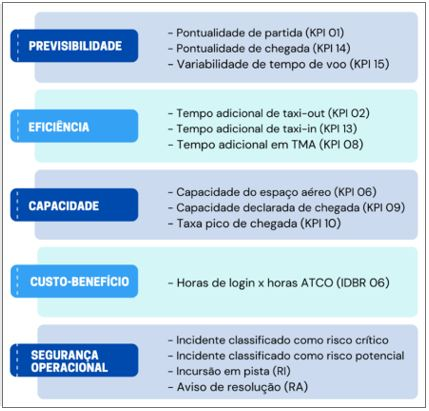
\includegraphics{imagens/fig1.jpg}
\caption{Imagem teste}
\end{figure}

A análise comparativa de desempenho entre os sistemas locais mostra as particularidades de cada órgão ATS, com semelhanças e diferenças na prestação do serviço de navegação aérea e na performance das Organizações Regionais. Entre as principais conclusões, destacam-se:

\begin{itemize}
\tightlist
\item
  Em geral, a prestação dos serviços de navegação aérea se reflete em um número mais elevado de controladores de tráfego aéreo (ATCO) nas regiões com maior densidade como a FIR-BS (CINDACTA I).
\item
  Em geral, a prestação dos serviços de navegação aérea se reflete em um número mais elevado de controladores de tráfego aéreo (ATCO) nas regiões com maior densidade como a FIR-BS (CINDACTA I).
\item
  As particularidades de cada Organização Regional ficam evidentes quando se confrontam números de movimentos por localidade ou por temporada; número de ATCO por localidade, por tamanho de região, por órgão, por total de movimentos, por complexidade ou por exigência do nível de inglês; por condições meteorológicas, dentre outras.
\item
  As capacidades de pista e de espaço aéreo estão projetadas para atender os níveis atuais de demanda, bem como o crescimento futuro de curto e médio prazos. Não houve mudanças significativas nos valores declarados de capacidade de espaço aéreo em 2022.
\item
  Em geral, o sistema apresentou associação entre menor demanda e maior eficiência, considerando especialmente os indicadores de pontualidade, de tempo adicional de táxi, de tempo adicional na terminal e de variabilidade de tempo de voo.
\item
  Considerando o escopo deste Relatório, os valores médios anuais encontrados no SISCEAB foram de: Pontualidade de Partida -- 84,3\% / Pontualidade de Chegada -- 67,7\% / Tempo Adicional de Taxi-out -- 3,65 min / Tempo Adicional de Taxi-in -- 1,75 min / Tempo Adicional de Chegada em TMA -- 4 min (C100) e 3 min (C40) / Índice de Operacionalidade dos ATCO -- 85,4\%.
\item
  Foram apresentadas algumas implantações recentes no SISCAB que podem ter impactado a performance geral do sistema ATM, incluindo uma abordagem inicial sobre os drones (UAS e derivados).
\end{itemize}

Este documento está organizado em cinco capítulos e dois anexos. No primeiro capítulo, é abordada a gestão por performance e apresentado um breve histórico falando sobre o GANP e ambições de desempenho, abordando-se, ainda, a abrangência, o âmbito geográfico, o escopo, o âmbito temporal, considerações sobre a retomada dos movimentos pós pandemia da COVID-19 (o ``novo normal'') e as fontes de dados utilizadas nas informações e indicadores apresentados.

O segundo capítulo apresenta as características do SISCEAB, apontando fatores internos e externos que podem influenciar nos resultados dos indicadores estudados, ressaltando como os serviços de navegação aérea são organizados e fazendo uma comparação geral das Organizações Regionais do DECEA. Além disso, inclui informações sobre a demanda nacional, desde o movimento nos principais aeroportos brasileiros, movimentos por segmento da aviação (Comercial Doméstica, Comercial Internacional e Geral), o ranking dos quarenta aeroportos mais movimentados, a participação dos movimentos por FIR, as rotas mais voadas pela aviação comercial, a densidade do tráfego aéreo nacional e sobre a composição da frota de aeronaves no país. São também abordados aspectos como a previsão quinquenal de demanda (nacional e por FIR), questões relacionadas ao ATCO, como efetivo e o nível de inglês, além da influência das condições meteorológicas nos aeroportos e um resumo dos principais projetos em andamento no SISCEAB.
No terceiro capítulo, são apresentados os resultados dos indicadores de performance ATM monitorados pelo DECEA em 2022, observando as metas publicadas no PCA 100-3, que abrangem as áreas de Previsibilidade, Eficiência, Capacidade, Custo-Benefício, Participação da Comunidade ATM, Segurança Operacional (Safety) e Segurança da Aviação (Security). Foram analisados os seguintes indicadores: KPI 01 -- Pontualidade de partida, KPI 14 -- Pontualidade de chegada, KPI 15 -- Variabilidade do tempo de voo, KPI 02 -- Tempo adicional de taxi-out, KPI 13 -- Tempo adicional de taxi-in, KPI 08 -- Tempo adicional em TMA, KPI 06 -- Capacidade do espaço aéreo, KPI 09 -- Capacidade declarada de chegada, KPI 10 -- Taxa-pico de chegada, Medidas ATFM, IDBR 06 -- Horas de LOGIN x Horas ATCO, IDBR 08 -- Índice de operacionalidade do ATCO, Pesquisa de Satisfação do SISCEAB, Incidente classificado como risco potencial, Incidente classificado como risco crítico, Incursão em pista e Aviso de resolução.

O quarto capítulo aponta as conclusões do estudo e as oportunidades de identificar melhorias a serem exploradas em prol do SISCEAB. No quinto capítulo são listadas as referências utilizadas para o desenvolvimento do trabalho.
Por fim, as Organizações Regionais do DECEA são apresentadas nos Anexos A e B. No primeiro anexo, tem-se o detalhamento de todos os órgãos ATS (ACC, APP, TWR, D-TWR, AFIS e R-AFIS), por Organização Regional do DECEA. No Anexo B são apresentadas de forma resumida as características das circulações aéreas nas FIR do espaço aéreo brasileiro.

Assim, o objetivo do Relatório de Performance ATM é fornecer uma visão geral da performance do SISCEAB, considerando os dados do ano de 2022, possibilitando uma análise gerencial macro do sistema, bem como de cada Organização Regional do DECEA.

\begin{figure}
\centering
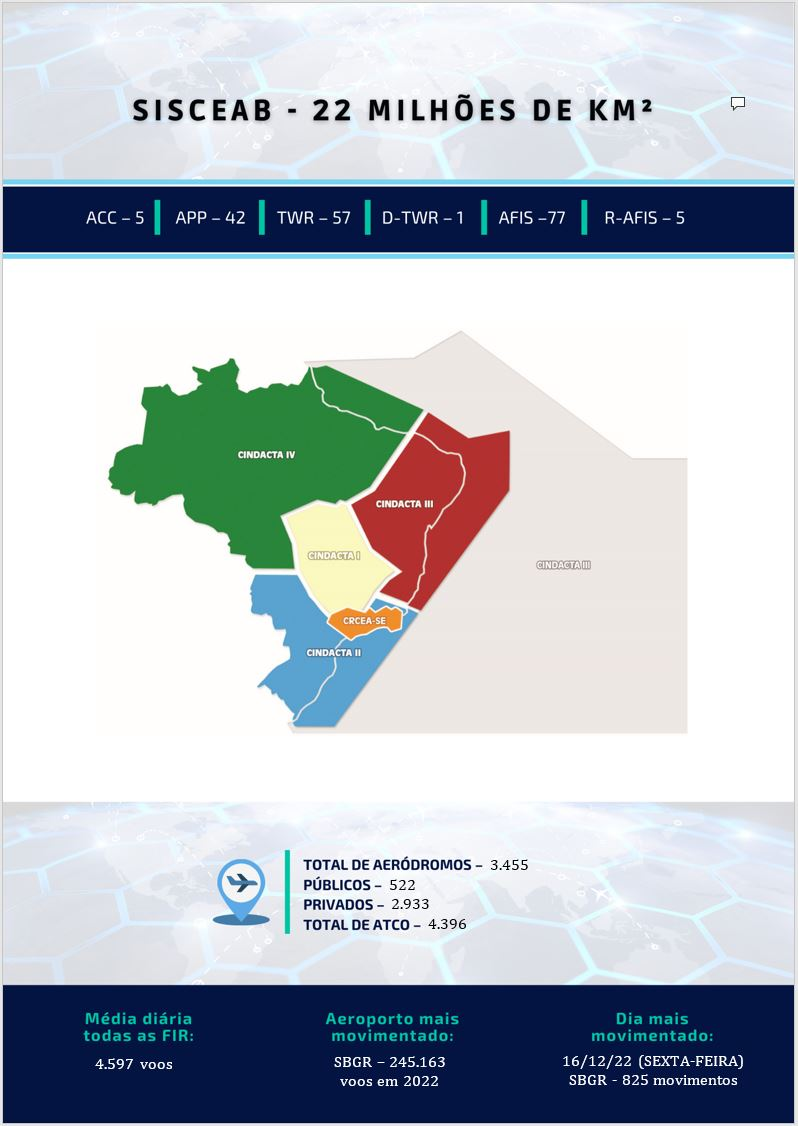
\includegraphics{imagens/fig2.jpg}
\caption{Imagem teste}
\end{figure}

\begin{figure}
\centering
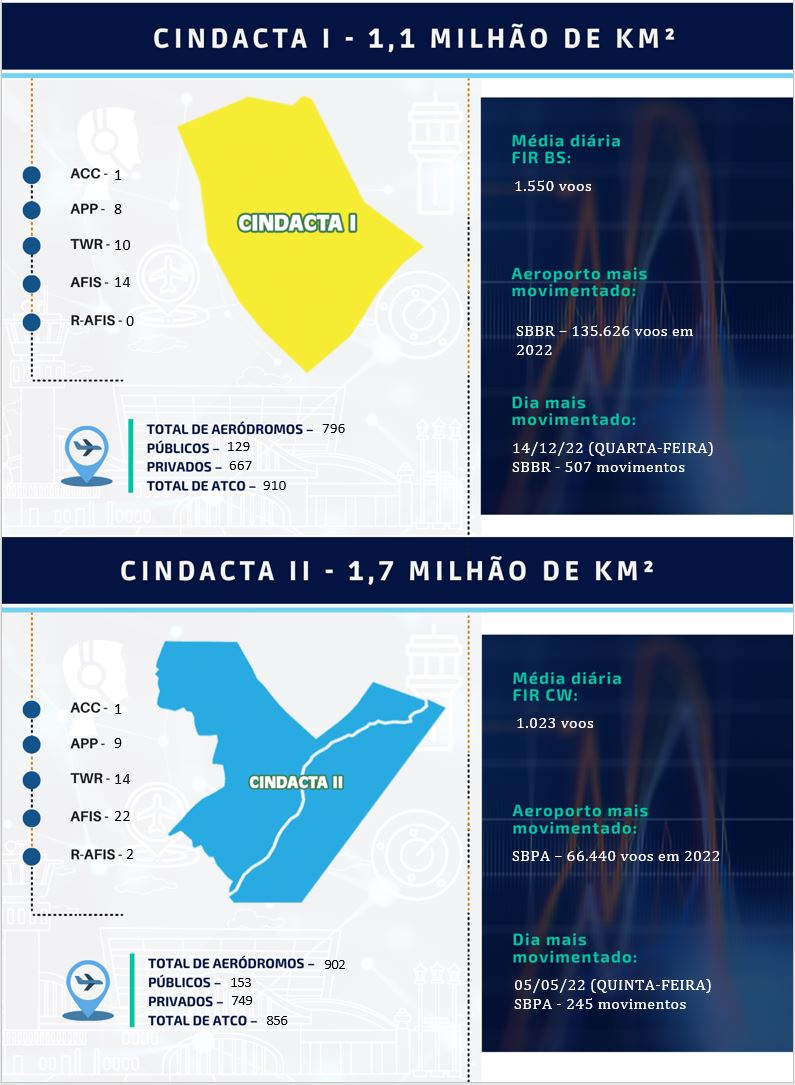
\includegraphics{imagens/fig3.jpg}
\caption{Imagem teste}
\end{figure}

\begin{figure}
\centering
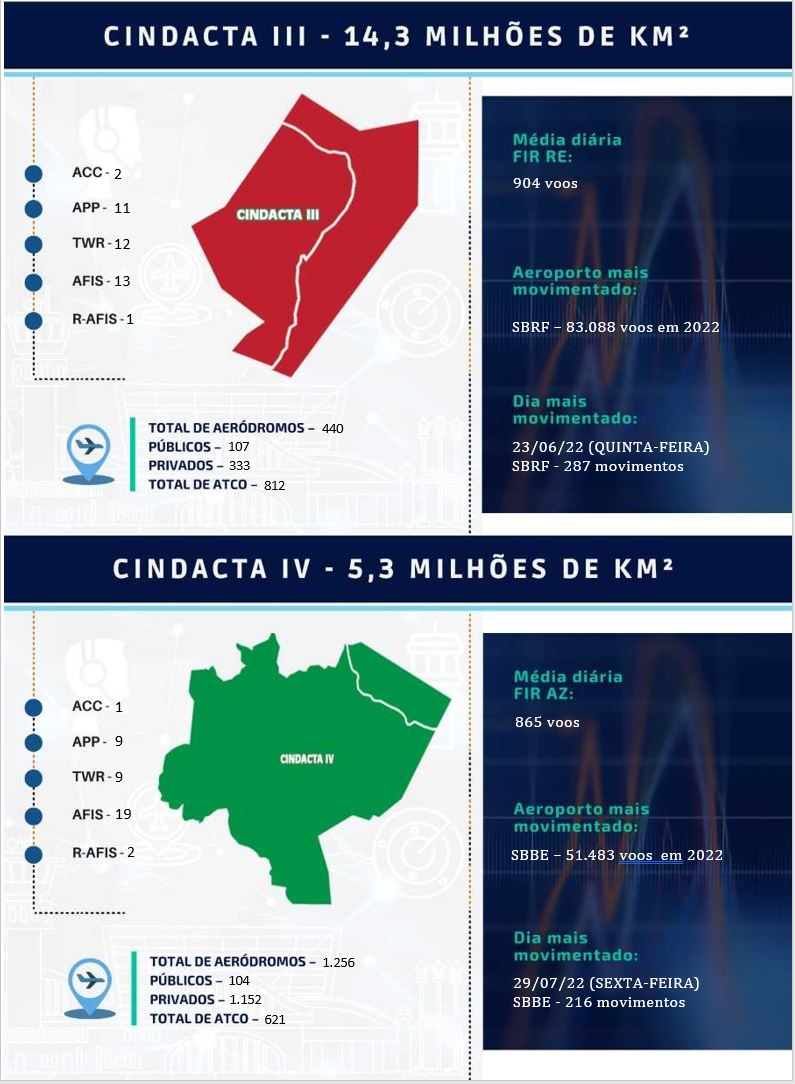
\includegraphics{imagens/fig4.jpg}
\caption{Imagem teste}
\end{figure}

\begin{figure}
\centering
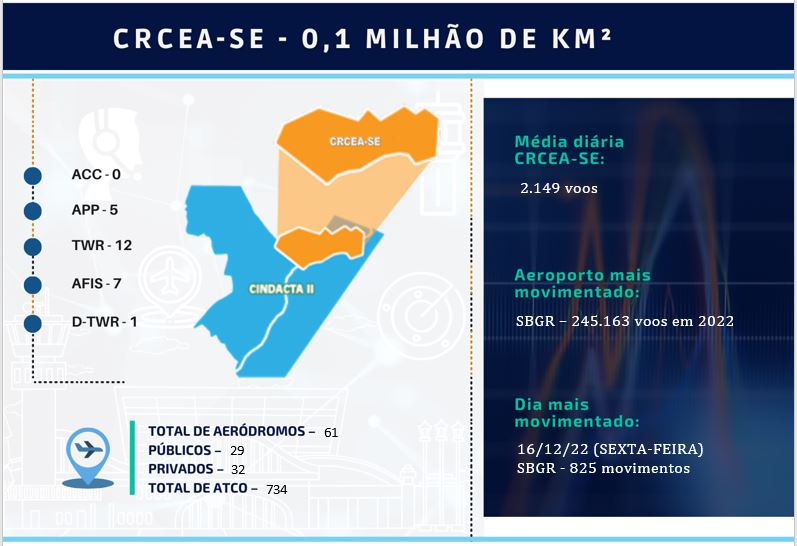
\includegraphics{imagens/fig5.jpg}
\caption{Imagem teste}
\end{figure}

Assim como nas edições anteriores do Relatório de Performance do SISCEAB, a análise comparativa entre as Organizações Regionais do DECEA inclui o Centro Regional de Controle do Espaço Aéreo do Sudeste (CRCEA-SE), destacando seu elevado número de movimentos nas áreas Terminais de São Paulo e do Rio de Janeiro. Cabe ressaltar, no entanto, que o CRCEA-SE gerencia porções de espaço aéreo que possuem caráter de área terminal (TMA), áreas significativamente menores que as Regiões de Informação de Voo sob jurisdição dos CINDACTA.

\begin{figure}
\centering
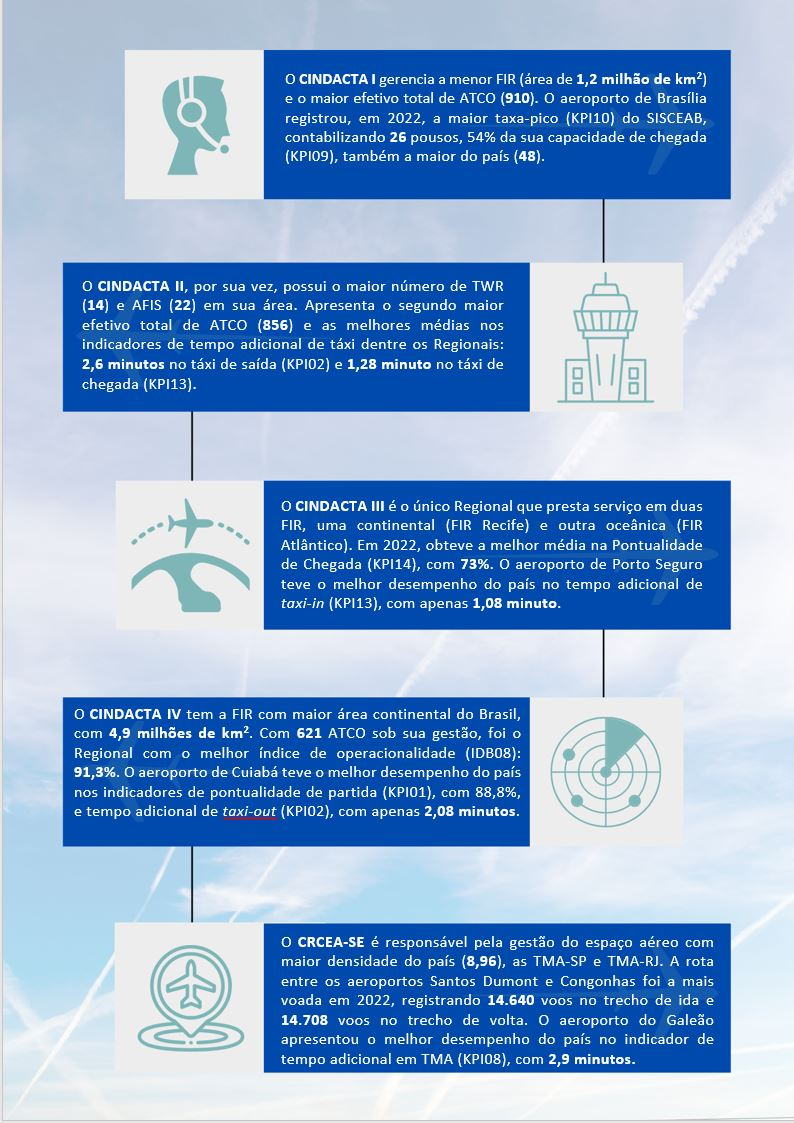
\includegraphics{imagens/fig6.jpg}
\caption{Imagem teste}
\end{figure}

\begin{verbatim}
<div align="center">
\end{verbatim}

\begin{figure}
\centering
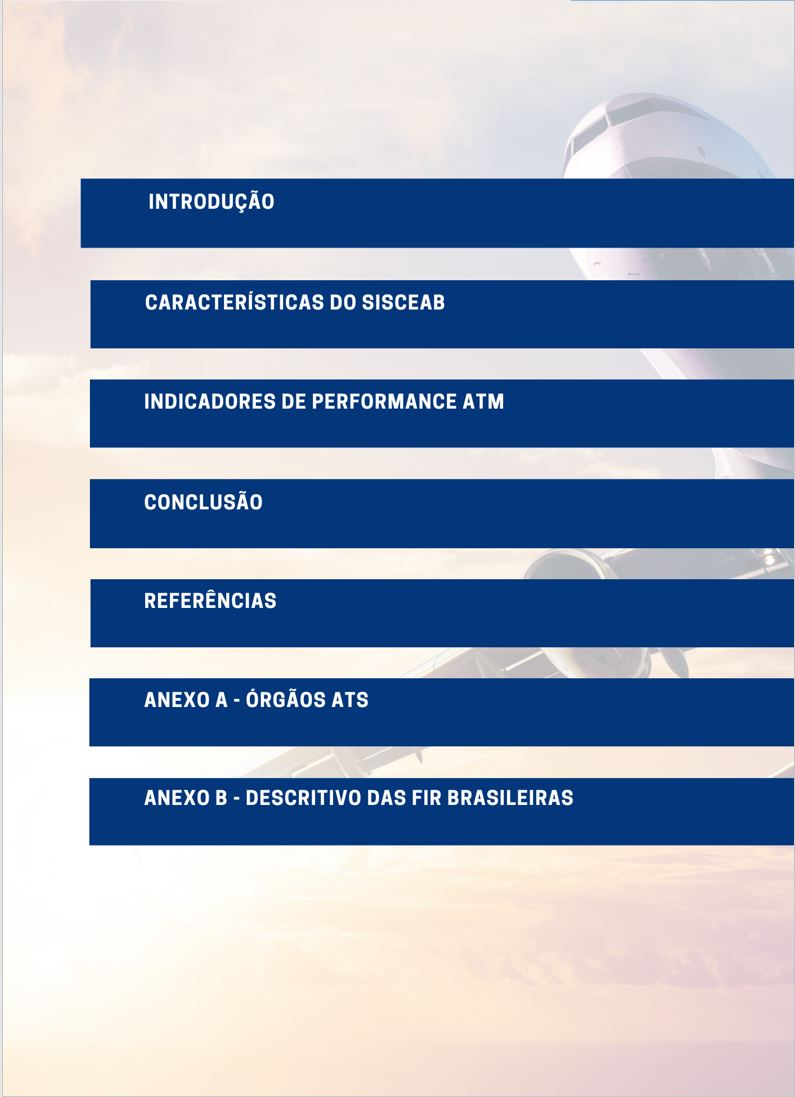
\includegraphics{imagens/fig7.jpg}
\caption{Imagem teste}
\end{figure}

\hypertarget{introduuxe7uxe3o}{%
\chapter{Introdução}\label{introduuxe7uxe3o}}

\hypertarget{gestuxe3o-por-performance}{%
\section{Gestão por performance}\label{gestuxe3o-por-performance}}

A Organização de Aviação Civil Internacional (OACI) é uma agência especializada das Nações Unidas que tem por objetivo desenvolver princípios e técnicas para a navegação aérea internacional fomentando o planejamento e o desenvolvimento do transporte aéreo global, promovendo o desenvolvimento de todos os aspectos da indústria de aviação civil internacional.

A OACI enfatiza a importância de uma gestão baseada em performance e estimula Estados, Regiões e Organizações a se envolverem e participarem de atividades de análise comparativa de desempenho, divulgando seus resultados para fornecer à comunidade ATM internacional uma oportunidade de monitorar a sua evolução.

Ao promover uma gestão por performance, os Estados são orientados a utilizarem um conjunto de indicadores-chave de performance (KPI -- Key Performance Indicators), que forneçam os meios de identificar deficiências e priorizar investimentos, além de compartilhar problemas de desempenho e melhores práticas em um nível regional e global, medindo e documentando os benefícios de desempenho produzidos pelas implementações de novas tecnologias e conceitos.

Desta forma, a gestão por performance permite que todas as partes envolvidas analisem a performance do sistema de navegação aérea corrente e futuro e tomem ações, caso necessário, de modo a preencher a lacuna entre o desempenho corrente e o desempenho esperado.

Assim, a CP-ATM, em atendimento ao Plano de Performance ATM do DECEA (PCA 100-3), dentre outras atribuições, atua na definição de indicadores de performance, na realização de análises pós-operações e em demais produtos de monitoramento do desempenho do SISCEAB, colaborando, assim, com a otimização da gestão por performance no âmbito do DECEA.

\hypertarget{plano-global-de-navegauxe7uxe3o-auxe9rea---ganp}{%
\subsection{Plano Global de Navegação Aérea - GANP}\label{plano-global-de-navegauxe7uxe3o-auxe9rea---ganp}}

O GANP é o mais alto documento estratégico de navegação aérea da OACI, constituindo diretrizes para conduzir a evolução do sistema global de navegação aérea e apoiando o planejamento para implementações em nível local (Estados isolados) e regional (grupos de Estados).

O objetivo do GANP é acomodar todas as operações dos usuários do espaço aéreo de maneira segura e economicamente viável, ao mesmo tempo em que busca a redução do impacto ambiental da aviação.

Este relatório de performance concentra-se em um subconjunto das onze Áreas de Performance (KPA) do GANP. A relação entre as áreas de desempenho e as ambições da comunidade ATM estão descritas no quadro a seguir.

\begin{longtable}[]{@{}
  >{\centering\arraybackslash}p{(\columnwidth - 2\tabcolsep) * \real{0.5000}}
  >{\centering\arraybackslash}p{(\columnwidth - 2\tabcolsep) * \real{0.5000}}@{}}
\toprule()
\begin{minipage}[b]{\linewidth}\centering
KPA
\end{minipage} & \begin{minipage}[b]{\linewidth}\centering
AMBIÇÃO DE DESEMPENHO
\end{minipage} \\
\midrule()
\endhead
ACESSO E EQUIDADE & Nenhum membro da comunidade aeronáutica excluído ou tratado de forma injusta \\
CAPACIDADE & Capacidade nominal facilmente compatível com a demanda. Eventos inesperados não interromperão a prestação do serviço e não afetarão significativamente o desempenho do sistema \\
CUSTO-BENEFÍCIO & Sem aumento do custo total direto dos Serviços de Navegação Aérea. Aumento significativo da produtividade dos Serviços de Navegação Aérea, independentemente da demanda \\
EFICIÊNCIA & Redução da distância entre a eficiência de voo alcançada e a trajetória ótima desejada \\
MEIO AMBIENTE & Ineficiências induzidas pelos Serviços de Navegação Aérea progressivamente eliminadas para contribuir com os objetivos globais da OACI relacionadas à emissões de CO2 Benefícios obtidos com os ganhos de eficiência de voo \\
FLEXIBILIDADE & Absorção das alterações necessárias às trajetórias dos voos \\
INTEROPERABILIDADE & Compatibilidade de sistemas em nível operacional e técnico \\
PARTICIPAÇÃO DA COMUNIDADE ATM & Máxima utilização partilhada dos recursos da navegação aérea \\
PREVISIBILIDADE & Sem variabilidade da entrega dos Serviços de Navegação Aérea \\
SEGURANÇA OPERACIONAL (Safety) & Sem acidentes relacionados com os Serviços de Navegação Aérea e redução significativa (50\%) dos incidentes graves \\
SEGURANÇA DA AVIAÇÃO (Security) & Sem interrupções significativas devido a incidentes cibernéticos \\
\bottomrule()
\end{longtable}

A visão do GANP reflete os objetivos do sistema de navegação aérea, que incluem desafios, oportunidades e tendências tecnológicas. A evolução impulsionada por essa visão produzirá um sistema de navegação aérea global de alto desempenho que atende às crescentes expectativas da sociedade.

Neste plano, é proposta uma estrutura de quatro camadas composta pelos níveis global (estratégico e técnico), regional e nacional, os quais fornecem uma estrutura para o alinhamento dos planos regionais, sub-regionais e nacionais. A estrutura de quatro camadas facilita a tomada de decisões ao fornecer uma direção estratégica estável para a evolução do sistema de navegação aérea e, ao mesmo tempo, indicando o grau de relevância, ao longo do tempo, para o conteúdo técnico a ser tratado.

\hypertarget{abranguxeancia}{%
\section{Abrangência}\label{abranguxeancia}}

Os indicadores de performance apresentados neste documento foram calculados por meio de informações coletadas das melhores fontes de dados em termos de qualidade, regularidade e disponibilidade. Comparações de atividades operacionais requerem padronização do modus operandi, definições e entendimento comuns, mesmo considerando as particularidades de cada localidade.

As informações descritas neste relatório não abordam todas as onze KPA previstas no GANP, concentrando-se nas informações relativas às características do sistema e nas áreas de Previsibilidade, Eficiência, Capacidade, Custo-Benefício, Segurança Operacional (Safety), Segurança da Aviação (Security) e Participação da Comunidade ATM. Além disso, projetos relacionados ao ATM também foram considerados.

\hypertarget{uxe2mbito-geogruxe1fico}{%
\section{Âmbito geográfico}\label{uxe2mbito-geogruxe1fico}}

Este relatório abrange todo o espaço aéreo sob responsabilidade do Brasil sobre terra e mar, que ultrapassa a área sobrejacente ao território brasileiro e alcança uma significativa parte do Oceano Atlântico, conforme tratados internacionais, estendendo-se além de suas fronteiras e perfazendo um total de 22 milhões de km2 sob gestão estratégica da Aeronáutica.

O controle do espaço aéreo brasileiro é integrado: as funções de Defesa Aérea e de Controle de Tráfego Aéreo são desempenhadas pelo DECEA, um órgão governamental subordinado ao Comando da Aeronáutica e ao Ministério da Defesa.

Ao DECEA compete a implementação de equipamentos, órgãos e sistemas, bem como o controle e a supervisão das Organizações subordinadas, provendo diretrizes estratégicas necessárias para a condução das ações executadas pelas suas Organizações Regionais, os quatro Centros Integrados de Defesa Aérea e Controle de Tráfego Aéreo (CINDACTA), distribuídos como áreas de responsabilidade próprias de cinco Regiões de Informação de Voo (FIR), e o Centro Regional de Controle do Espaço Aéreo Sudeste (CRCEA-SE), com as seguintes estruturas de jurisdição:

\hypertarget{escopo}{%
\section{Escopo}\label{escopo}}

O escopo de análise foi definido pela necessidade de identificar um conjunto comum de fontes de dados com níveis de detalhamento e cobertura adequados. Atendendo ao previsto no PCA 100-3, dentro das KPA já mencionadas, fazem parte do escopo do relatório as seguintes localidades:

\begin{figure}
\centering
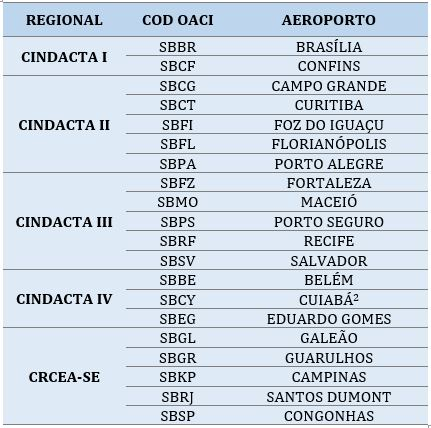
\includegraphics{imagens/fig8.jpg}
\caption{Imagem teste}
\end{figure}

\hypertarget{uxe2mbito-temporal}{%
\section{Âmbito temporal}\label{uxe2mbito-temporal}}

Este relatório aborda o desempenho monitorado no SISCEAB para o período de 1º JAN 2022 a 31 DEZ 2022.

\hypertarget{retomada-da-demanda-nacional-puxf3s-covid-19}{%
\section{Retomada da demanda nacional pós-COVID-19}\label{retomada-da-demanda-nacional-puxf3s-covid-19}}

Os impactos da pandemia da COVID-19 na indústria do transporte aéreo foram significativos e sem precedentes, estendendo-se durante a maior parte de 2020 e por todo o ano de 2021. A aviação internacional foi o segmento que mais sofreu com as medidas sanitárias impostas, em função do surgimento de novas variantes e do aumento no número de casos.

A Erro! Autoreferência de indicador não válida. apresenta o total de voos realizados no SISCEAB em 2022, considerando os serviços prestados pelos diversos órgãos de controle. É possível observar a retomada das operações aéreas em quase todos os meses do último ano, com operações sempre próximas ou acima do total de 2019 (pré-pandemia). Vale ressaltar que o ``Total de Voos no SISCEAB'' conta todos os voos realizados no país, em espaço aéreo controlado, a partir dos planos de voo ativos. Adiante, ao se analisar no 2.4.1 as operações por segmento da aviação (Comercial Doméstica, Comercial Internacional e Geral), são consideradas as operações de pouso e decolagem nos principais aeroportos do país.

Os meses de maior movimento em 2022 foram julho e agosto, registrando 153.915 e 150.258 voos, respectivamente. Ao final do ano, o total de operações aéreas no SISCEAB ficou 5,2\% acima do total de 2019.

\begin{figure}

{\centering 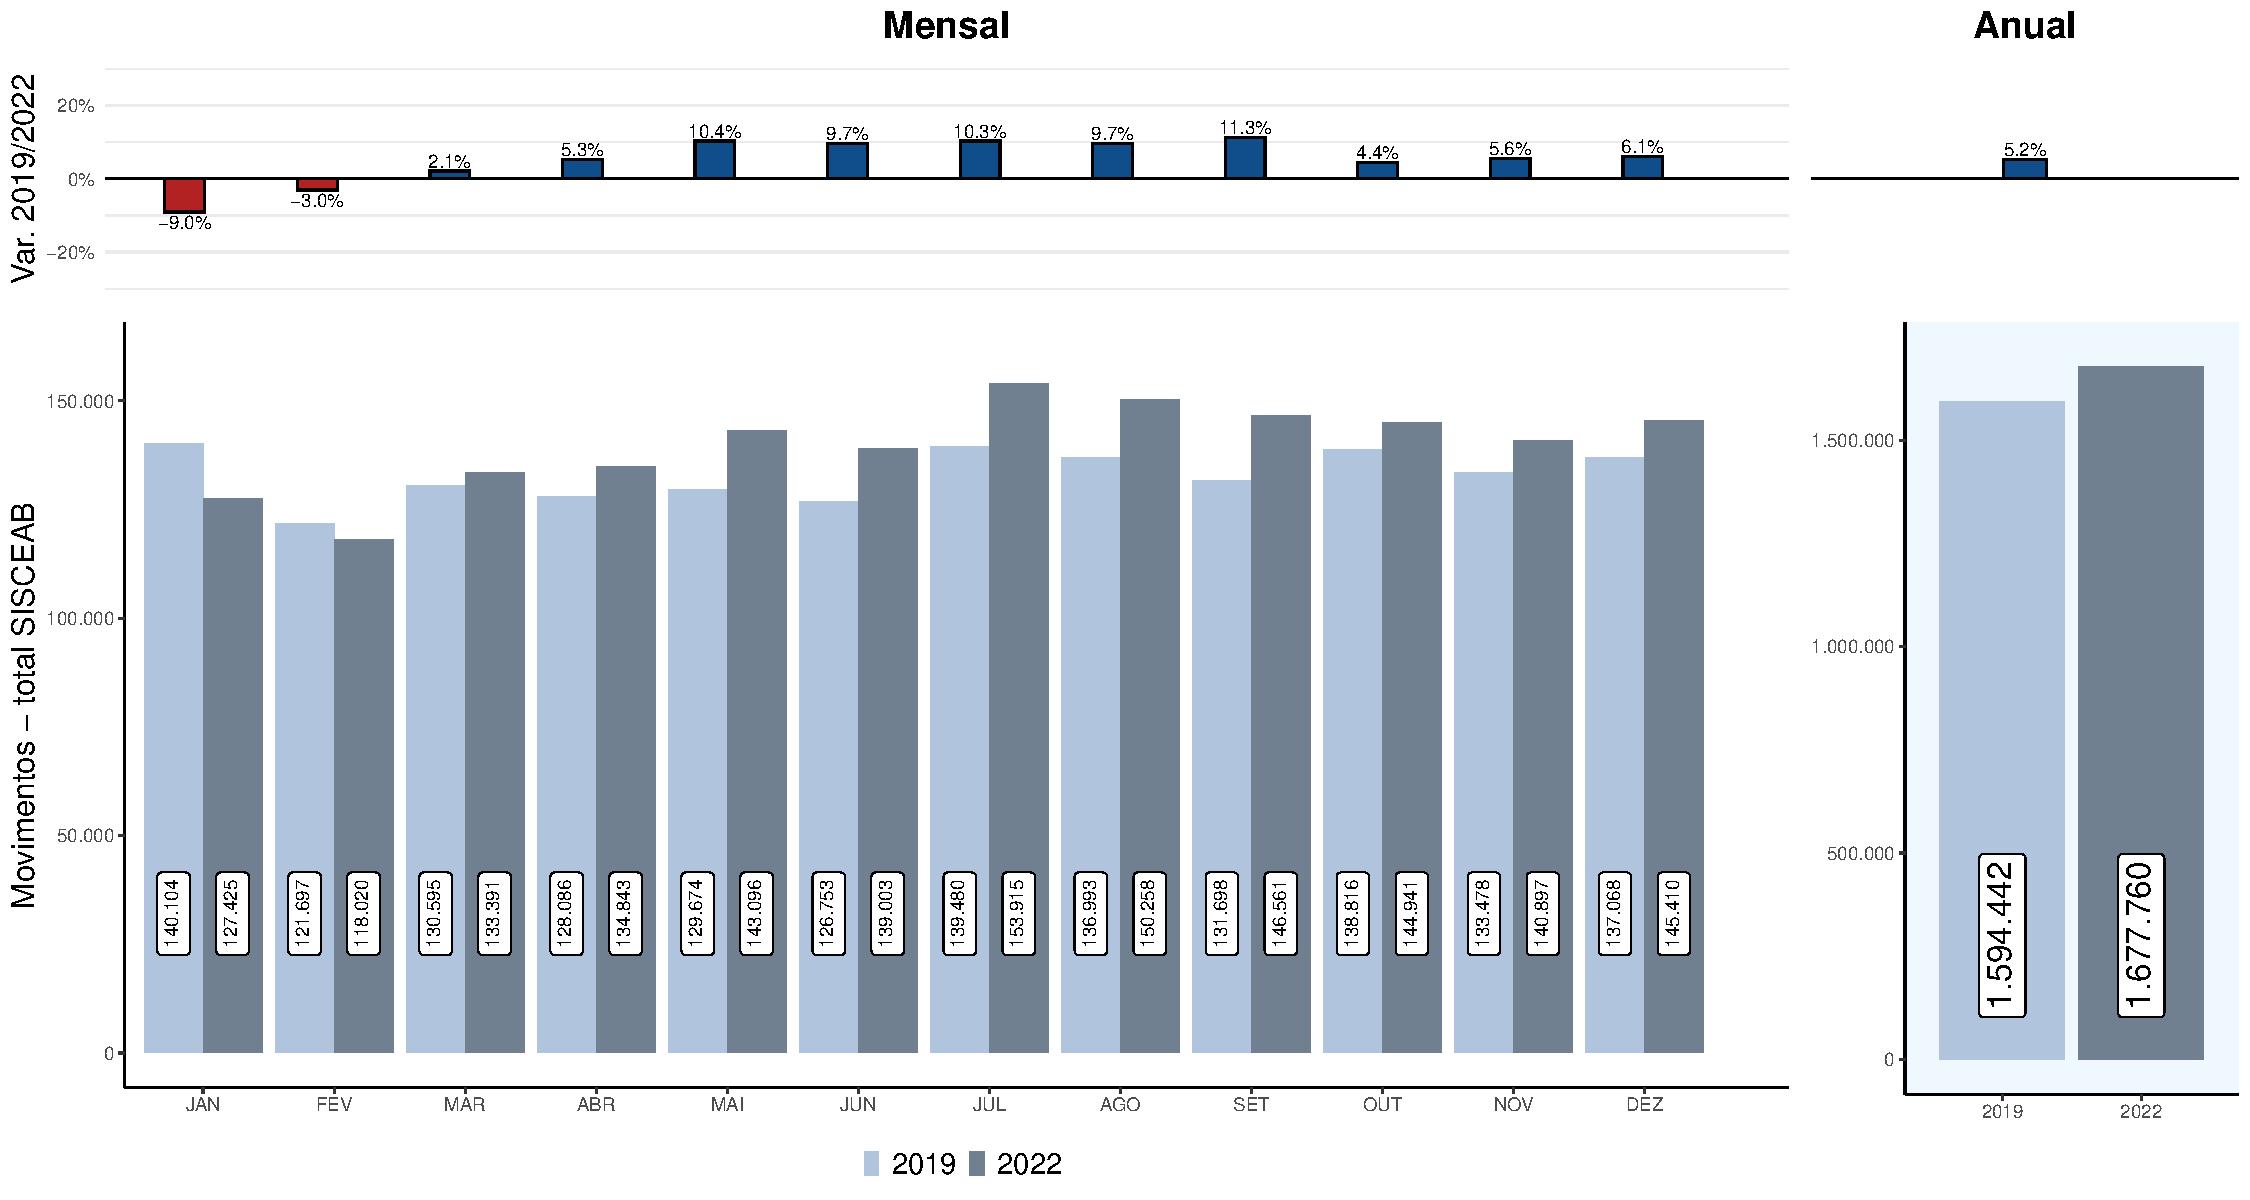
\includegraphics{_main_files/figure-latex/gf.1, -1} 

}

\caption{Total de voos no SISCEAB}(\#fig:gf.1, )
\end{figure}

\hypertarget{fontes-de-dados}{%
\section{Fontes de dados}\label{fontes-de-dados}}

Os indicadores de performance ATM analisados neste relatório, bem como os dados de movimentos de tráfego aéreo e outras informações abordadas baseiam-se nas fontes de dados elencadas no quadro abaixo.

\begin{figure}
\centering
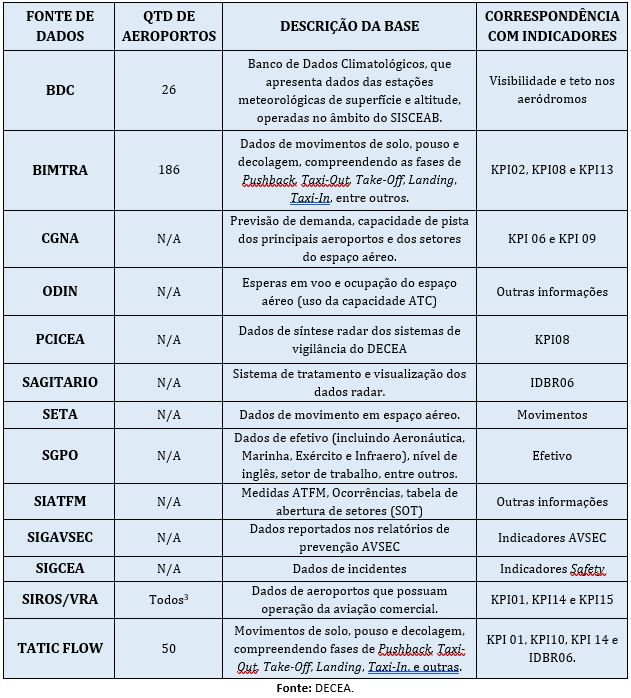
\includegraphics{imagens/fig9.jpg}
\caption{Imagem teste}
\end{figure}

Destaca-se que o Manual de Metodologia de Indicadores ATM do SISCEAB (MCA 100-22), disponível no portal AISWEB do DECEA, contém a descrição completa de cada indicador de performance ATM abordado neste documento, bem como a respectiva fonte de dados.

É importante reforçar a informação sobre mudanças de algumas fontes de dados para determinados indicadores e informações do Relatório de Performance ATM de 2021 (edição anterior a esta), em relação aos documentos publicados em anos anteriores. Essas alterações ocorreram como resultado do aprimoramento da Subdivisão de Pós-Operações do CGNA e da Divisão de Pesquisas do Instituto de Controle do Espaço Aéreo (ICEA) na mineração, no tratamento e no armazenamento dos dados coletados das diversas fontes do SISCEAB, e contemplam os resultados publicados no Relatório de Performance ATM de 2022.

\hypertarget{cross}{%
\chapter{Características do SISCEAB}\label{cross}}

O SISCEAB compreende uma área extensa, revelando características singulares entre as Organizações Regionais do DECEA em termos de:

\begin{itemize}
\tightlist
\item
  Organização dos Serviços de Tráfego Aéreo (ATS);
\item
  Tipos de órgãos ATS;
\item
  Características do sistema ATM;
\item
  Perfil atual e futuro da demanda;
\item
  Efetivo de Controlador de Tráfego Aéreo (ATCO);
\item
  Fatores meteorológicos; e
\item
  Projetos no SISCEAB.
\end{itemize}

Tais particularidades são abordadas ao longo deste capítulo em face da influência que esses fatores têm nos indicadores de performance ATM.

As características dos aeródromos, das TMA e das FIR, bem como suas respectivas complexidades e carga de trabalho associada, podem indicar a necessidade de alocar um efetivo maior de ATCO em determinados órgãos de controle, independentemente do tamanho da área geográfica sob sua jurisdição.

\begin{figure}
\centering
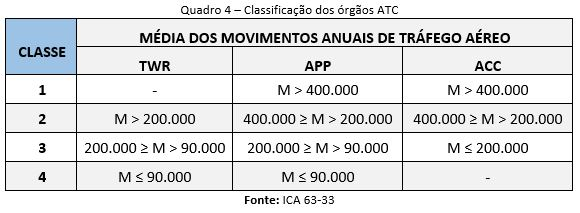
\includegraphics{imagens/fig10.jpg}
\caption{Imagem teste}
\end{figure}

A quantidade de movimentos anuais dos principais aeroportos, das TWR, dos APP e dos ACC pode ser conferida no Anuário Estatístico de Tráfego Aéreo, documento produzido pelo CGNA e disponível em \url{http://portal.cgna.decea.mil.br}, na aba Recursos, ou em \url{http://performance.decea.mil.br/} , na aba Produtos.

\hypertarget{organizauxe7uxe3o-dos-serviuxe7os-de-navegauxe7uxe3o-auxe9rea}{%
\section{Organização dos Serviços de Navegação Aérea}\label{organizauxe7uxe3o-dos-serviuxe7os-de-navegauxe7uxe3o-auxe9rea}}

O DECEA é o órgão central do SISCEAB, responsável pela gestão do tráfego aéreo, que envolve todas as atividades relacionadas à segurança e à eficiência do controle do espaço aéreo brasileiro.

O espaço aéreo sob responsabilidade do Brasil é uma área de aproximadamente 22 milhões de km2, organizada em cinco Regiões de Informação de Voo (FIR), contendo cinco Centros de Controle de Área (ACC), 42 Controles de Aproximação (APP), 57 Torres de Controle de Aeródromo (TWR), uma Torre de Controle Digital (D-TWR), 75 Rádios (AFIS) e cinco Rádios Remotas (R-AFIS).

O CGNA é a organização responsável pelo serviço de Gerenciamento de Fluxo de Tráfego Aéreo (ATFM) no espaço aéreo brasileiro, aplicando medidas ATFM, quando necessário, e conduzindo o processo de tomada de decisões colaborativas com a Comunidade ATM nacional (companhias aéreas, aeroportos, órgãos de controle etc.). Além disso, também coordena a gestão do espaço aéreo, o sistema de tratamento de planos de voo, o banco de dados estatísticos, as análises de indicadores e pós-operações, bem como outras atividades relacionadas à navegação aérea.

\hypertarget{uxf3rguxe3os-ats-acc-app-twr-afis}{%
\section{Órgãos ATS -- ACC / APP / TWR / AFIS}\label{uxf3rguxe3os-ats-acc-app-twr-afis}}

Os órgãos ATS prestam os Serviços de Tráfego Aéreo, que incluem os Serviços de Controle de Tráfego Aéreo, de Informação de Voo e de Alerta.
Popularmente, o tema controle de tráfego aéreo é associado à figura de uma torre de controle (TWR).

Entretanto, a TWR é uma das engrenagens do grande sistema que compõe o SISCEAB, no qual, também estão envolvidos órgãos de controle como os Centros de Controle de Área (ACC) e os Controles de Aproximação (APP). Adicionalmente, existem as Rádios que, por sua vez, são órgãos prestadores do Serviço de Informação de Voo de Aeródromo (AFIS) que complementam os órgãos provedores dos Serviços de Tráfego Aéreo (ATS).

Cada um desses órgãos ATS possui a sua respectiva área de jurisdição, regulamentos inerentes ao serviço prestado e equipamentos adequados para o provimento de suas atribuições. O ANEXO A apresenta os Regionais e os respectivos órgãos ATS sob sua jurisdição.

\hypertarget{centro-de-controle-de-uxe1rea-acc}{%
\section{Centro de Controle de Área -- ACC}\label{centro-de-controle-de-uxe1rea-acc}}

O ACC é um órgão de controle de tráfego aéreo encarregado de prestar os Serviços ATS às aeronaves que evoluem na Região de Informação de Voo (FIR). A FIR é uma porção do espaço aéreo com grandes dimensões em que ocorrem as fases de subida, descida, sobrevoo e cruzamento entre diferentes aeronaves, com performances distintas e em níveis de voo variados.

Os ACC brasileiros trabalham ininterruptamente com equipes de controladores de tráfego aéreo, militares especialistas da Aeronáutica que se revezam em turnos específicos de serviço.

Os ACC dispõem de modernas tecnologias para o provimento seguro, ordenado e rápido do tráfego aéreo. Dentre esses recursos, destacam-se:

\begin{itemize}
\tightlist
\item
  SAGITARIO -- Sistema Avançado de Gerenciamento de Informações de Tráfego Aéreo e Relatório de Interesse Operacional;
\item
  CPDLC -- Comunicações por Enlace de Dados Controlador-Piloto; e
\item
  ADS-C -- Vigilância Dependente Automática -- Contrato.
\end{itemize}

\hypertarget{controle-de-aproximauxe7uxe3o---app}{%
\section{Controle de Aproximação - APP}\label{controle-de-aproximauxe7uxe3o---app}}

O APP é um órgão de controle de tráfego aéreo encarregado de prestar os serviços requeridos pelas aeronaves partindo e chegando nos aeroportos situados no interior de uma área de controle terminal.

No Brasil, os APP contam com equipes de ATCO, compostas por militares especialistas da Aeronáutica, da Marinha do Brasil ou do Exército Brasileiro. Adicionalmente, alguns APP são integrados por profissionais civis, oriundos de outros Provedores de Serviços de Navegação Aérea (PSNA) como, por exemplo, a NAV Brasil e a INFRAERO. Mesmo com entidades externas ao Comando da Aeronáutica , todo o processo de formação de controladores bem como a gestão de licenças e habilitações é realizada pelo DECEA.

Os APP brasileiros dispõem de modernas tecnologias para o provimento seguro, ordenado e rápido do tráfego aéreo. Dentre esses recursos, destacam-se:

\begin{itemize}
\tightlist
\item
  SAGITARIO (sistema de visualização dos dados radar);
\item
  AMAN (Sistema de Gerenciamento de Chegada);
\item
  SITTI (Central de áudio/telefonia integrada); e
\item
  ADS-B (Vigilância Dependente Automática por Radiodifusão).
\end{itemize}

\hypertarget{torre-de-controle-de-aeruxf3dromo---twr}{%
\section{Torre de Controle de Aeródromo - TWR}\label{torre-de-controle-de-aeruxf3dromo---twr}}

A TWR é um órgão de controle de tráfego aéreo situada nos aeroportos de maior movimento.

De modo geral, a TWR é responsável por prestar os serviços requeridos pelas aeronaves apenas durante as fases de decolagem e pouso em um aeródromo. Incluem-se entre esses serviços o controle no solo de viaturas e pessoas na área de manobras e, quando necessário, o controle dos voos no circuito de tráfego visual do aeródromo.

Da mesma forma que ocorre com os APP, as TWR do Brasil também contam com equipes de ATCO que podem ser especialistas da Aeronáutica ou profissionais de entidades externas.

Adicionalmente, a incorporação de novas tecnologias ATM, como, por exemplo, o TATIC-TWR, o DCL (autorização de tráfego via enlace de dados) e o radar de solo, permitem otimizar a segurança, a eficiência e o gerenciamento em TWR de elevado fluxo de aeronaves.

Alinhando recursos tecnológicos atuais com práticas inovadoras, o DECEA implementou, no aeródromo de Santa Cruz, a primeira Torre Digital (D-TWR) do SISCEAB.

Na operação da D-TWR Santa Cruz, a visualização tradicional do ATCO acerca do cenário operacional foi substituída pela visualização de um sistema de vigilância, composto por câmeras de alta resolução e monitores, que proporcionam aos controladores uma visão panorâmica do aeródromo e de sua vizinhança.

A primeira D-TWR brasileira foi mais um grande passo à modernização da infraestrutura aeroportuária nacional, permitindo fomentar experiências e conhecimentos para futuras aplicações nos demais aeródromos do país.

Nos aeroportos cujo volume de operações aéreas é considerado baixo, não existe necessidade de instalação de uma TWR. Nesses casos, é disponibilizado o AFIS, cujo serviço é prestado por Operadores de Estação Aeronáutica.

No Brasil, as estações aeronáuticas são identificadas como Rádios e prestam o Serviço de Informação de Voo de Aeródromo (AFIS) visando proporcionar informações relevantes aos aeronavegantes.

Eventualmente, alguns APP ou TWR, em determinados horários e de acordo com critérios estabelecidos, podem prestar o AFIS. Isso permite modular o serviço prestado em função da demanda existente, racionalizando recursos, sem prejuízo à segurança operacional.

A partir de 2016, foram viabilizados os órgãos AFIS remotos (R-AFIS) em aeroportos de baixo movimento, sendo o serviço prestado de forma remota à localidade. Atualmente, as localidades de Fernando de Noronha (na FIR-RE), Oiapoque e Vilhena (na FIR-AZ), Uruguaiana e Corumbá (na FIR-CW) operam na configuração R-AFIS.

As Rádios, remotas ou não, contam com equipes de Operadores de Estação Aeronáutica, que podem ser militares ou civis, da Aeronáutica ou de outras organizações.

\hypertarget{afis}{%
\section{AFIS}\label{afis}}

No Brasil, as estações aeronáuticas são identificadas como Rádios e prestam o Serviço de Informação de Voo de Aeródromo (AFIS) visando proporcionar informações relevantes aos aeronavegantes.

Eventualmente, alguns APP ou TWR, em determinados horários e de acordo com critérios estabelecidos, podem prestar o AFIS. Isso permite modular o serviço prestado em função da demanda existente, racionalizando recursos, sem prejuízo à segurança operacional.

A partir de 2016, foram viabilizados os órgãos AFIS remotos (R-AFIS) em aeroportos de baixo movimento, sendo o serviço prestado de forma remota à localidade. Atualmente, as localidades de Fernando de Noronha (na FIR-RE), Oiapoque e Vilhena (na FIR-AZ), Uruguaiana e Corumbá (na FIR-CW) operam na configuração R-AFIS.

As Rádios, remotas ou não, contam com equipes de Operadores de Estação Aeronáutica, que podem ser militares ou civis, da Aeronáutica ou de outras organizações.

\hypertarget{organizauxe7uxf5es-regionais-do-decea}{%
\section{Organizações Regionais do DECEA}\label{organizauxe7uxf5es-regionais-do-decea}}

O Quadro 5 apresenta as principais características do sistema ATM brasileiro, que permite identificar o cenário de cada Organização Regional.

\begin{figure}
\centering
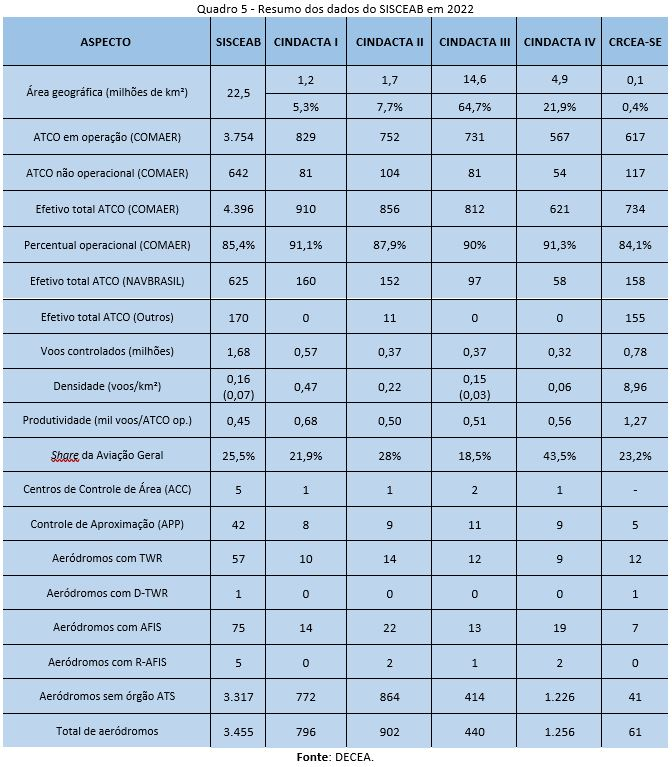
\includegraphics{imagens/fig11.jpg}
\caption{Imagem teste}
\end{figure}

\textbf{NOTA 1:} A metodologia que mede a área geográfica de cada Regional sofreu uma pequena modificação: no Relatório de 2021, se utilizou o critério da jurisdição, que excluía a área do CRCEA-SE das FIR sobrejacentes. Nesta edição, foi utilizada a delimitação geográfica de cada FIR. Assim, a área do CRCEA-SE deixa de ser agregada no cômputo geral do SISCEAB, que é igual ao somatório de suas cinco FIR.

\textbf{NOTA 2:} Em 2022, houve redimensionamento das FIR Amazônica, Atlântico e Recife. Em 16 de junho, parte da FIR-AZ passou para a FIR-AO. Em 1º de dezembro de 2022, parte da FIR-AO passou para a FIR-RE.

\textbf{NOTA 3:} As informações relativas aos ATCO foram extraídas do Sistema de Gestão de Pessoal Operacional (SGPO), com base nos detentores de licença de ATCO em atividade, sendo incluídos os graduados militares BCT (da ativa ou da reserva), estagiários, ATCO de Defesa Aérea, oficiais CTA e civis DACTA contabilizados em cada Regional. No efetivo total do SISCEAB e no percentual operacional, além dos ATCO já informados nos Regionais, são considerados também os militares alocados em unidades fora dos Regionais, mas não são considerados aqueles em formação na Escola de Especialistas de Aeronáutica (EEAR). Foram incluídas informações específicas sobre operadores de outras Forças, da NAVBRASIL e demais PSNA.

\textbf{NOTA 4:} Em relação aos voos controlados, a quantidade de voos foi calculada por FIR/Regional, com base no número de movimentos de 1º/01/2022 a 31/12/2022 constantes no SETA Millenium, excluindo-se os movimentos repetidos nas duas bases (das localidades de origem e de destino).

\textbf{NOTA 5:} Os dados descritos na NOTA 4 foram utilizados para o cálculo da densidade, em número de voos/km2. A partir daí, foi considerada a inclusão da área da FIR-AO, representada com os valores entre parênteses (0,07 para o SISCEAB e 0,03 para o CINDACTA III). Assim, os valores sem os parênteses representam a densidade do SISCEAB e do CINDACTA III desconsiderando a área da FIR-AO.

\textbf{NOTA 6:} A produtividade foi calculada na grandeza de mil voos por ATCO operacional.

\textbf{NOTA 7:} O share da aviação geral indica a participação deste segmento em relação ao total de movimentos.

\textbf{NOTA 8:} Em relação ao número de ACC, APP, TWR e AFIS, as informações foram obtidas nas publicações AIP-Brasil, ROTAER e no Portal AISWEB, do DECEA, conforme o ANEXO A.

\textbf{NOTA 9:} A quantidade de aeródromos foi contabilizada de acordo com o site de performance do DECEA. Para o cálculo do quantitativo de aeródromos sem órgãos ATS foi considerado o total de aeródromos que não possuem TWR, D-TWR, AFIS e R-AFIS.

\hypertarget{caracterizauxe7uxe3o-da-demanda}{%
\section{Caracterização da demanda}\label{caracterizauxe7uxe3o-da-demanda}}

O objetivo geral dos serviços de tráfego aéreo é o fornecimento de um fluxo de tráfego aéreo seguro, ordenado e eficiente. Para fins de comparações operacionais, é importante ter um bom entendimento da demanda nos principais aeroportos do SISCEAB, do ranking dos aeroportos, da participação de movimentos por FIR, das rotas mais voadas pela aviação comercial, da densidade do tráfego e como a frota é composta, de acordo com a classificação das aeronaves em leve, média ou pesada.

A caracterização da demanda de tráfego aéreo no Brasil é detalhada nos tópicos a seguir.

\begin{figure}
\centering
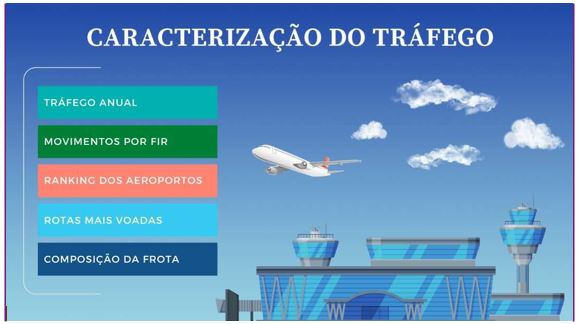
\includegraphics{imagens/fig12.jpg}
\caption{Imagem teste}
\end{figure}

\hypertarget{demanda-nos-principais-aeroportos-do-sisceab}{%
\subsection{Demanda nos principais aeroportos do SISCEAB}\label{demanda-nos-principais-aeroportos-do-sisceab}}

Em 2022, a demanda nos principais aeroportos brasileiros apresentou números muito próximos ao volume de operações aéreas observado em 2019, ano de referência pré-pandemia. Nessa seção, são considerados os 34 principais aeroportos, contabilizando as respectivas operações de pouso e decolagem.

Nesse sentido, a Figura 3 apresenta a média móvel semanal de pousos e decolagens realizados nos principais aeroportos do SISCEAB nos últimos anos. Em 2019, foi observada pouca variação ao longo do ano, com uma média em torno de 5.500 operações de pousos e decolagens por dia. A partir de março de 2020, observa-se uma queda significativa na média móvel em função da pandemia da COVID-19. No ano seguinte, apesar da recuperação inicial, os meses de março, abril e maio mostraram novas contrações da demanda em virtude da segunda onda da COVID-19.

Ao fim do ano passado, a média móvel de operações nos principais aeroportos estava acima de 5.000 movimentos por dia, caracterizando, assim, a recuperação da demanda nacional e a retomada dos voos no cenário pós-covid (o ``novo normal'').

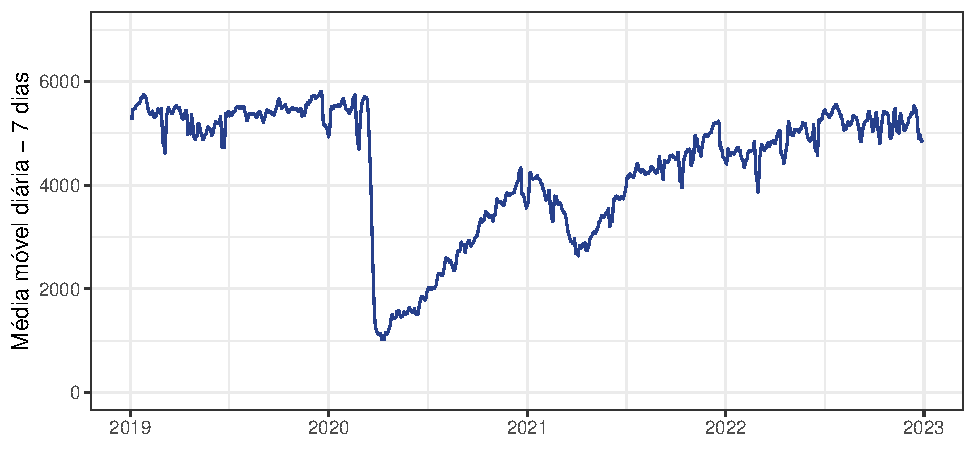
\includegraphics{_main_files/figure-latex/unnamed-chunk-3-1.pdf}

\hypertarget{aviauxe7uxe3o-comercial-domuxe9stica}{%
\subsubsection{Aviação comercial doméstica}\label{aviauxe7uxe3o-comercial-domuxe9stica}}

A Erro! Autoreferência de indicador não válida. apresenta o volume de operações de pouso e decolagem nos principais aeroportos brasileiros e a variação observada ao comparar 2022 com 2019. Pode-se verificar que a demanda comercial doméstica operou acima de 90\% do volume de 2019 de maio a dezembro de 2022, sendo maio o mês com o melhor desempenho (apenas 2,9\% abaixo do volume de 2019).

A aviação comercial doméstica nos principais aeroportos brasileiros operou com 89,8\% do volume pré-pandemia (10,2\% abaixo do volume de 2019).

\hypertarget{chapters-and-sub-chapters}{%
\section{Chapters and sub-chapters}\label{chapters-and-sub-chapters}}

There are two steps to cross-reference any heading:

\begin{enumerate}
\def\labelenumi{\arabic{enumi}.}
\tightlist
\item
  Label the heading: \texttt{\#\ Hello\ world\ \{\#nice-label\}}.

  \begin{itemize}
  \tightlist
  \item
    Leave the label off if you like the automated heading generated based on your heading title: for example, \texttt{\#\ Hello\ world} = \texttt{\#\ Hello\ world\ \{\#hello-world\}}.
  \item
    To label an un-numbered heading, use: \texttt{\#\ Hello\ world\ \{-\#nice-label\}} or \texttt{\{\#\ Hello\ world\ .unnumbered\}}.
  \end{itemize}
\item
  Next, reference the labeled heading anywhere in the text using \texttt{\textbackslash{}@ref(nice-label)}; for example, please see Chapter \ref{cross}.

  \begin{itemize}
  \tightlist
  \item
    If you prefer text as the link instead of a numbered reference use: \protect\hyperlink{cross}{any text you want can go here}.
  \end{itemize}
\end{enumerate}

\hypertarget{captioned-figures-and-tables}{%
\section{Captioned figures and tables}\label{captioned-figures-and-tables}}

Figures and tables \emph{with captions} can also be cross-referenced from elsewhere in your book using \texttt{\textbackslash{}@ref(fig:chunk-label)} and \texttt{\textbackslash{}@ref(tab:chunk-label)}, respectively.

See Figure \ref{fig:nice-fig}.

\begin{Shaded}
\begin{Highlighting}[]
\FunctionTok{par}\NormalTok{(}\AttributeTok{mar =} \FunctionTok{c}\NormalTok{(}\DecValTok{4}\NormalTok{, }\DecValTok{4}\NormalTok{, .}\DecValTok{1}\NormalTok{, .}\DecValTok{1}\NormalTok{))}
\FunctionTok{plot}\NormalTok{(pressure, }\AttributeTok{type =} \StringTok{\textquotesingle{}b\textquotesingle{}}\NormalTok{, }\AttributeTok{pch =} \DecValTok{19}\NormalTok{)}
\end{Highlighting}
\end{Shaded}

\begin{figure}

{\centering 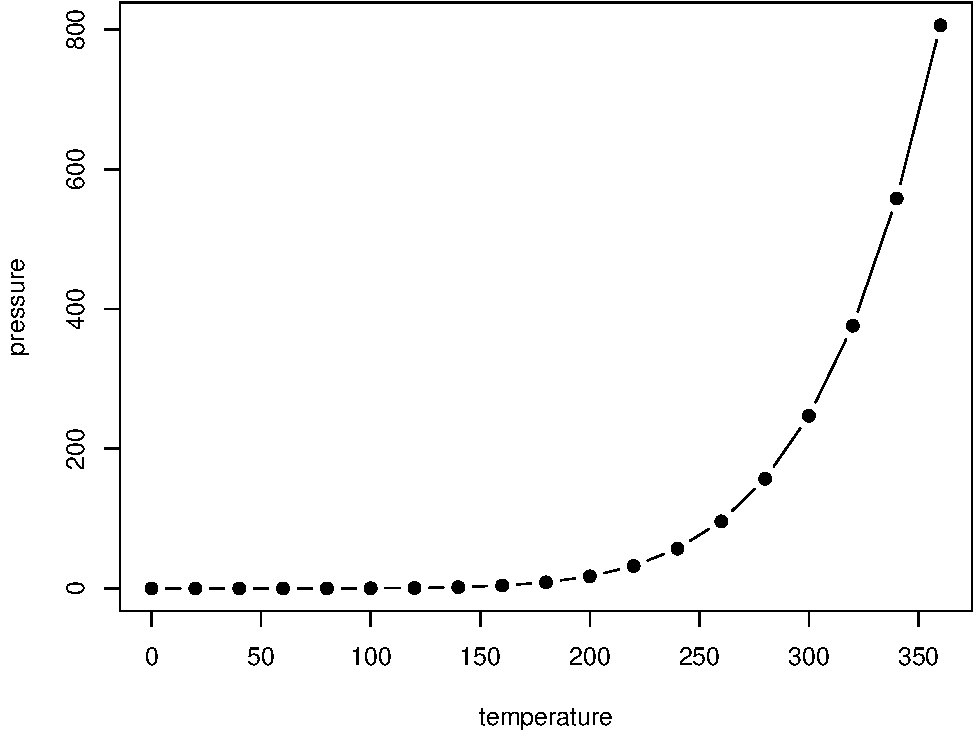
\includegraphics[width=0.8\linewidth]{_main_files/figure-latex/nice-fig-1} 

}

\caption{Here is a nice figure!}\label{fig:nice-fig}
\end{figure}

Don't miss Table \ref{tab:nice-tab}.

\begin{Shaded}
\begin{Highlighting}[]
\NormalTok{knitr}\SpecialCharTok{::}\FunctionTok{kable}\NormalTok{(}
  \FunctionTok{head}\NormalTok{(pressure, }\DecValTok{10}\NormalTok{), }\AttributeTok{caption =} \StringTok{\textquotesingle{}Here is a nice table!\textquotesingle{}}\NormalTok{,}
  \AttributeTok{booktabs =} \ConstantTok{TRUE}
\NormalTok{)}
\end{Highlighting}
\end{Shaded}

\begin{table}

\caption{\label{tab:nice-tab}Here is a nice table!}
\centering
\begin{tabular}[t]{rr}
\toprule
temperature & pressure\\
\midrule
0 & 0.0002\\
20 & 0.0012\\
40 & 0.0060\\
60 & 0.0300\\
80 & 0.0900\\
\addlinespace
100 & 0.2700\\
120 & 0.7500\\
140 & 1.8500\\
160 & 4.2000\\
180 & 8.8000\\
\bottomrule
\end{tabular}
\end{table}

\hypertarget{parts}{%
\chapter{Parts}\label{parts}}

You can add parts to organize one or more book chapters together. Parts can be inserted at the top of an .Rmd file, before the first-level chapter heading in that same file.

Add a numbered part: \texttt{\#\ (PART)\ Act\ one\ \{-\}} (followed by \texttt{\#\ A\ chapter})

Add an unnumbered part: \texttt{\#\ (PART\textbackslash{}*)\ Act\ one\ \{-\}} (followed by \texttt{\#\ A\ chapter})

Add an appendix as a special kind of un-numbered part: \texttt{\#\ (APPENDIX)\ Other\ stuff\ \{-\}} (followed by \texttt{\#\ A\ chapter}). Chapters in an appendix are prepended with letters instead of numbers.

\hypertarget{footnotes-and-citations}{%
\chapter{Footnotes and citations}\label{footnotes-and-citations}}

\hypertarget{footnotes}{%
\section{Footnotes}\label{footnotes}}

Footnotes are put inside the square brackets after a caret \texttt{\^{}{[}{]}}. Like this one \footnote{This is a footnote.}.

\hypertarget{citations}{%
\section{Citations}\label{citations}}

Reference items in your bibliography file(s) using \texttt{@key}.

For example, we are using the \textbf{bookdown} package \citep{R-bookdown} (check out the last code chunk in index.Rmd to see how this citation key was added) in this sample book, which was built on top of R Markdown and \textbf{knitr} \citep{xie2015} (this citation was added manually in an external file book.bib).
Note that the \texttt{.bib} files need to be listed in the index.Rmd with the YAML \texttt{bibliography} key.

The RStudio Visual Markdown Editor can also make it easier to insert citations: \url{https://rstudio.github.io/visual-markdown-editing/\#/citations}

\hypertarget{blocks}{%
\chapter{Blocks}\label{blocks}}

\hypertarget{equations}{%
\section{Equations}\label{equations}}

Here is an equation.

\begin{equation} 
  f\left(k\right) = \binom{n}{k} p^k\left(1-p\right)^{n-k}
  \label{eq:binom}
\end{equation}

You may refer to using \texttt{\textbackslash{}@ref(eq:binom)}, like see Equation \eqref{eq:binom}.

\hypertarget{theorems-and-proofs}{%
\section{Theorems and proofs}\label{theorems-and-proofs}}

Labeled theorems can be referenced in text using \texttt{\textbackslash{}@ref(thm:tri)}, for example, check out this smart theorem \ref{thm:tri}.

\begin{theorem}
\protect\hypertarget{thm:tri}{}\label{thm:tri}For a right triangle, if \(c\) denotes the \emph{length} of the hypotenuse
and \(a\) and \(b\) denote the lengths of the \textbf{other} two sides, we have
\[a^2 + b^2 = c^2\]
\end{theorem}

Read more here \url{https://bookdown.org/yihui/bookdown/markdown-extensions-by-bookdown.html}.

\hypertarget{callout-blocks}{%
\section{Callout blocks}\label{callout-blocks}}

The R Markdown Cookbook provides more help on how to use custom blocks to design your own callouts: \url{https://bookdown.org/yihui/rmarkdown-cookbook/custom-blocks.html}

\hypertarget{sharing-your-book}{%
\chapter{Sharing your book}\label{sharing-your-book}}

\hypertarget{publishing}{%
\section{Publishing}\label{publishing}}

HTML books can be published online, see: \url{https://bookdown.org/yihui/bookdown/publishing.html}

\hypertarget{pages}{%
\section{404 pages}\label{pages}}

By default, users will be directed to a 404 page if they try to access a webpage that cannot be found. If you'd like to customize your 404 page instead of using the default, you may add either a \texttt{\_404.Rmd} or \texttt{\_404.md} file to your project root and use code and/or Markdown syntax.

\hypertarget{metadata-for-sharing}{%
\section{Metadata for sharing}\label{metadata-for-sharing}}

Bookdown HTML books will provide HTML metadata for social sharing on platforms like Twitter, Facebook, and LinkedIn, using information you provide in the \texttt{index.Rmd} YAML. To setup, set the \texttt{url} for your book and the path to your \texttt{cover-image} file. Your book's \texttt{title} and \texttt{description} are also used.

This \texttt{gitbook} uses the same social sharing data across all chapters in your book- all links shared will look the same.

Specify your book's source repository on GitHub using the \texttt{edit} key under the configuration options in the \texttt{\_output.yml} file, which allows users to suggest an edit by linking to a chapter's source file.

Read more about the features of this output format here:

\url{https://pkgs.rstudio.com/bookdown/reference/gitbook.html}

Or use:

\begin{Shaded}
\begin{Highlighting}[]
\NormalTok{?bookdown}\SpecialCharTok{::}\NormalTok{gitbook}
\end{Highlighting}
\end{Shaded}

\#1. BDS

\hypertarget{gruxe1fico-movimento-da-aviauxe7uxe3o-comercial-domuxe9stica}{%
\chapter{2 GRÁFICO MOVIMENTO DA AVIAÇÃO COMERCIAL DOMÉSTICA}\label{gruxe1fico-movimento-da-aviauxe7uxe3o-comercial-domuxe9stica}}

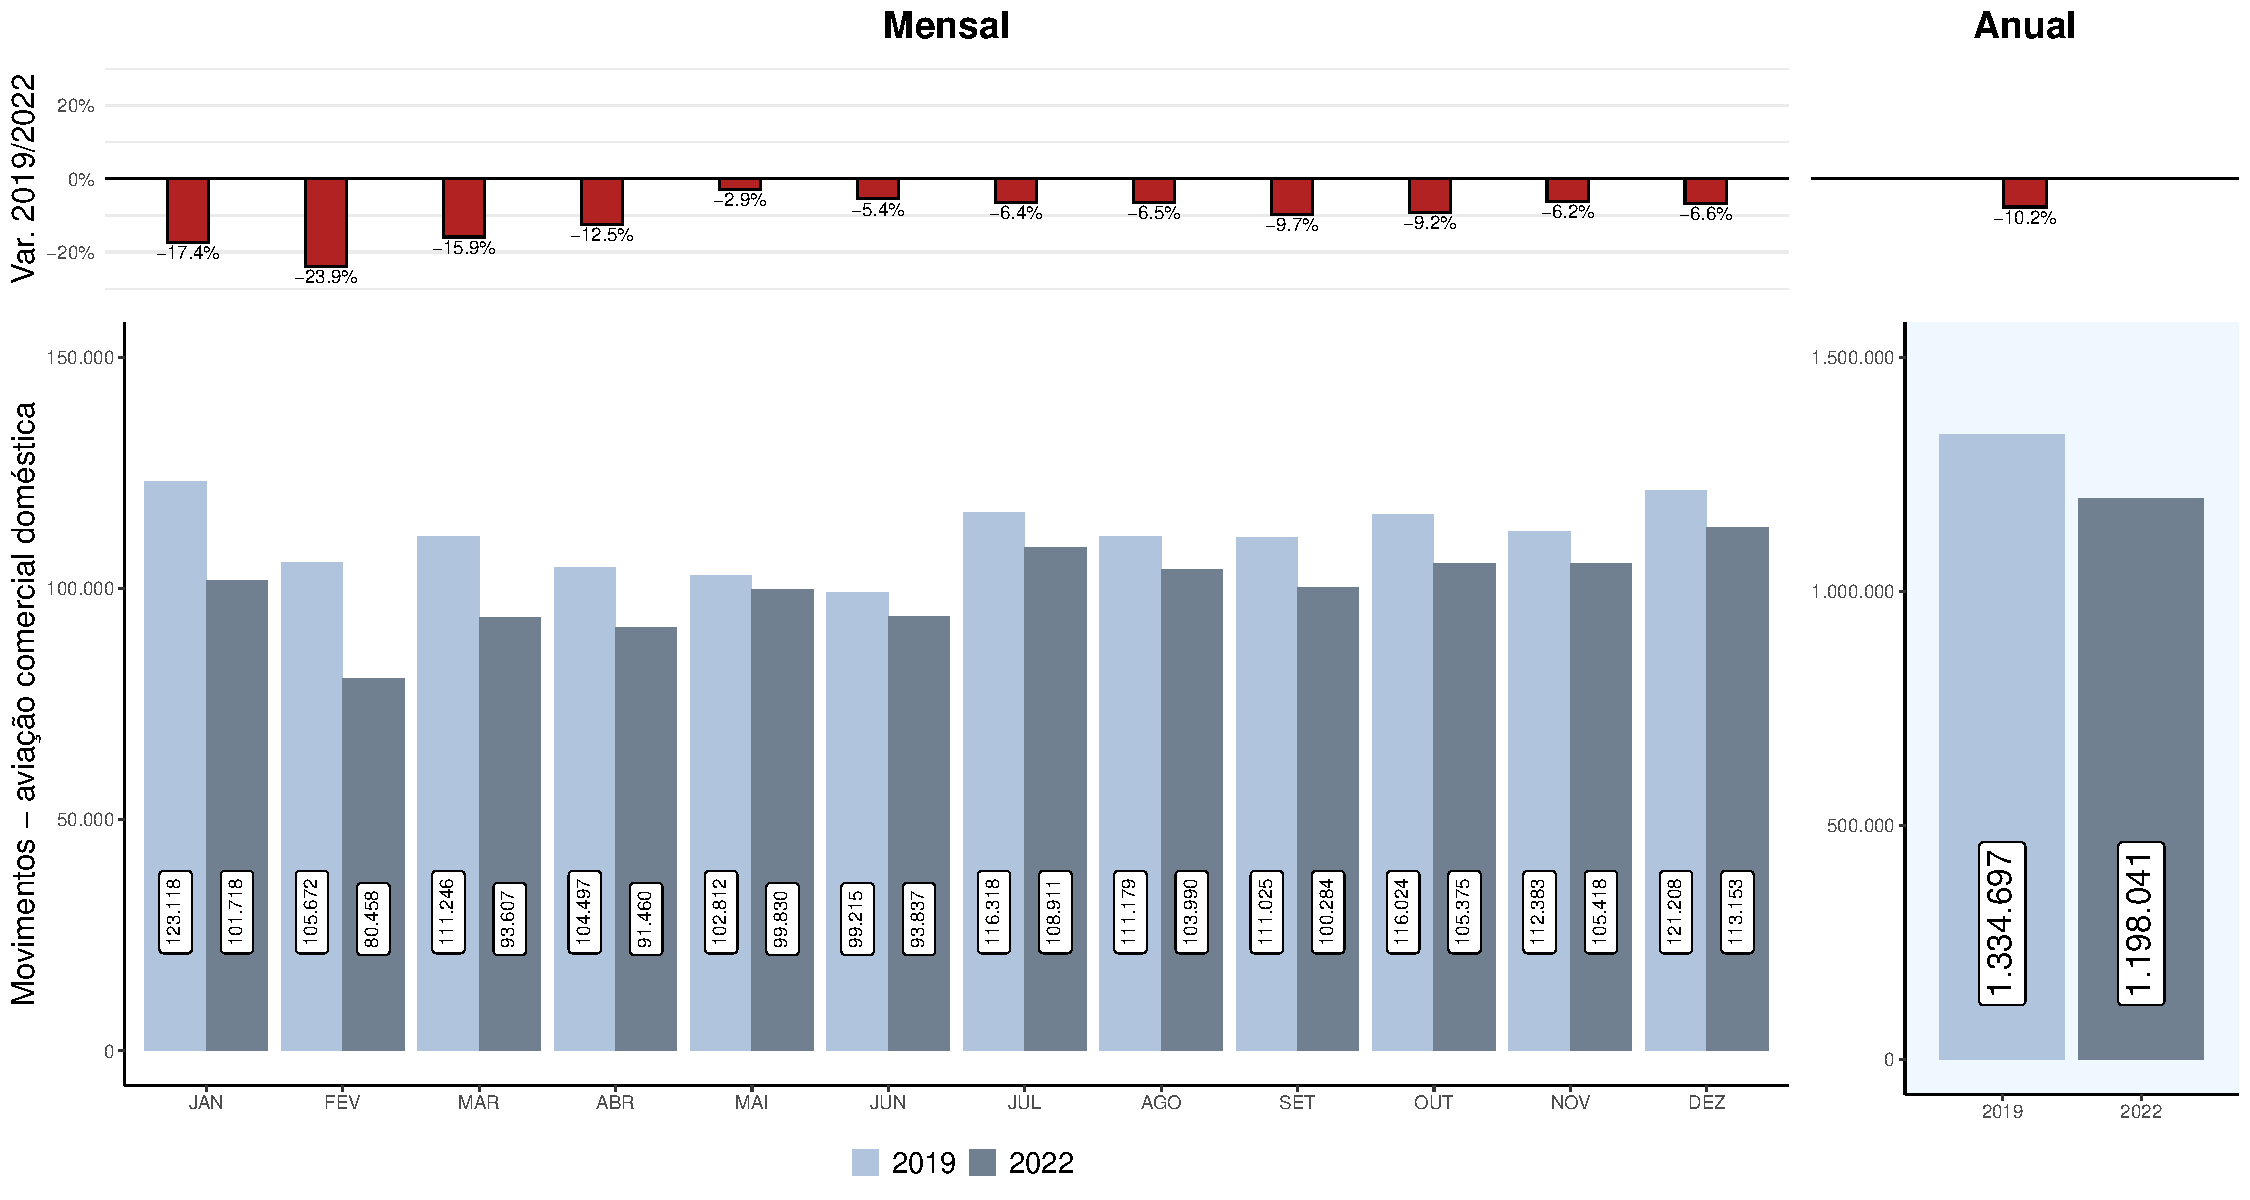
\includegraphics{_main_files/figure-latex/unnamed-chunk-7-1.pdf}

\#3 GRÁFICO MOVIMENTO AVIAÇÃO COMERCIAL INTERNACIONAL

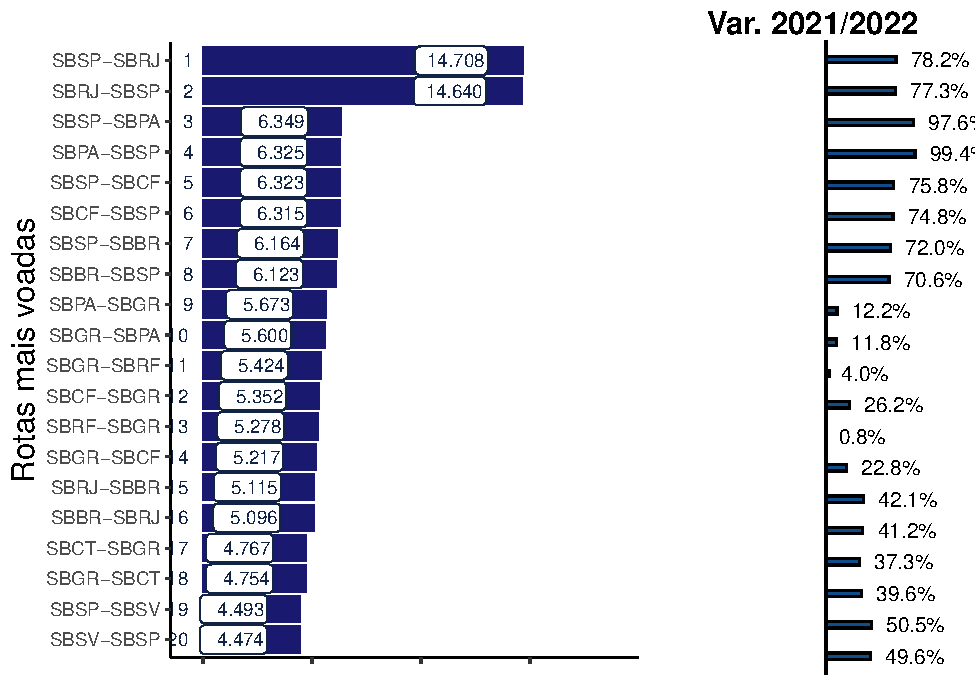
\includegraphics{_main_files/figure-latex/unnamed-chunk-8-1.pdf}

\hypertarget{gruxe1fico-de-movimento-da-aviauxe7uxe3o-geral}{%
\chapter{4 GRÁFICO DE MOVIMENTO DA AVIAÇÃO GERAL}\label{gruxe1fico-de-movimento-da-aviauxe7uxe3o-geral}}

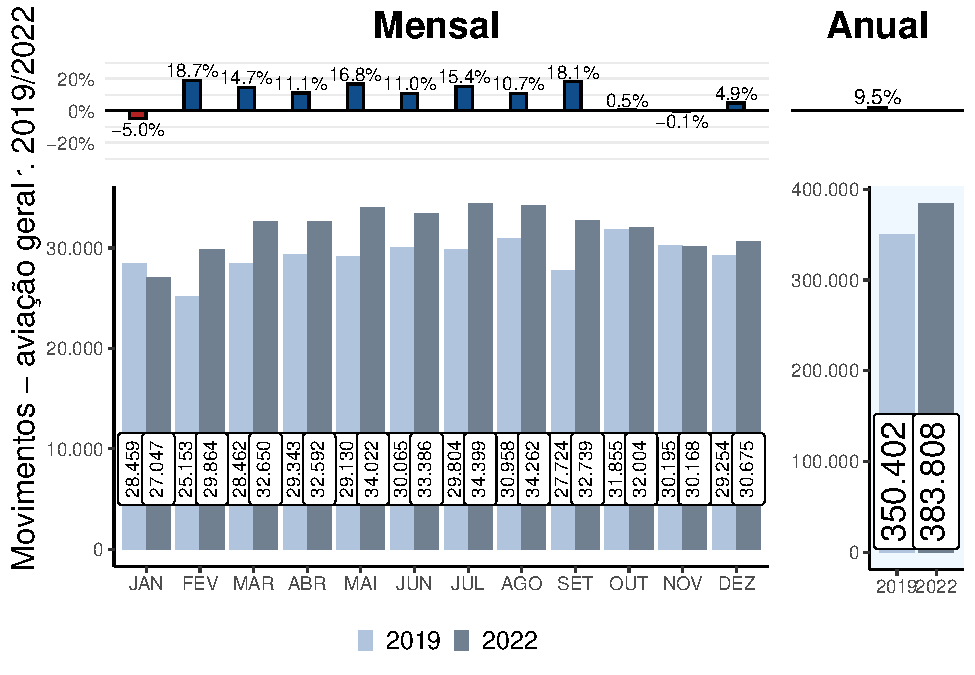
\includegraphics{_main_files/figure-latex/unnamed-chunk-9-1.pdf}

\#\#4.1 GRÁFICO COMPARATIVO POR MÊS DE TOTAL DE OPERAÇÕES ARR E DEP NO SISCEAB

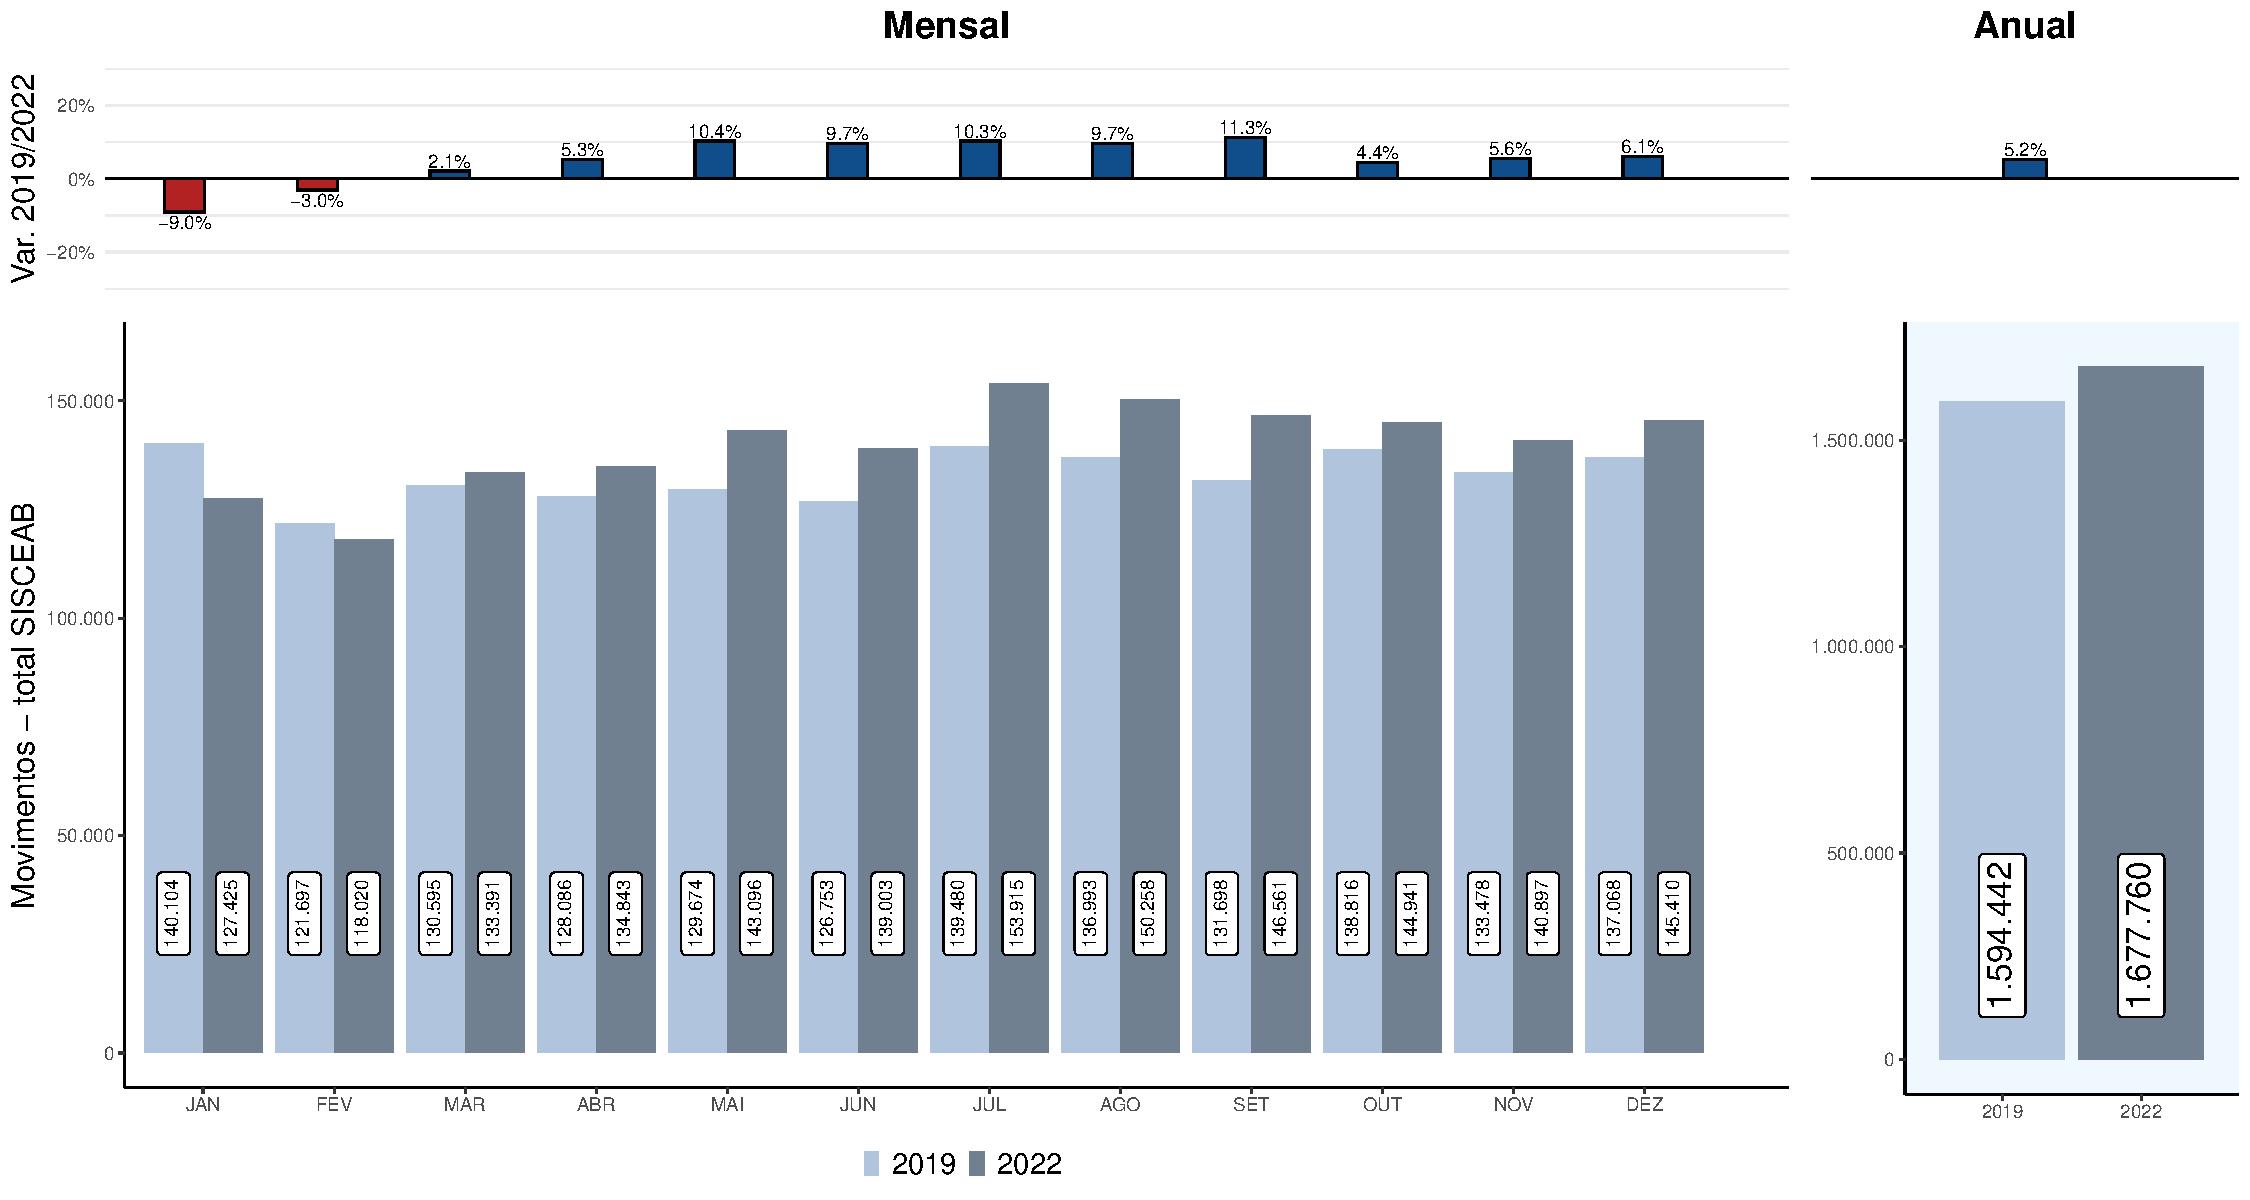
\includegraphics{_main_files/figure-latex/unnamed-chunk-10-1.pdf}

\#5 GRÁFICO DE MOVIMENTOS FIR

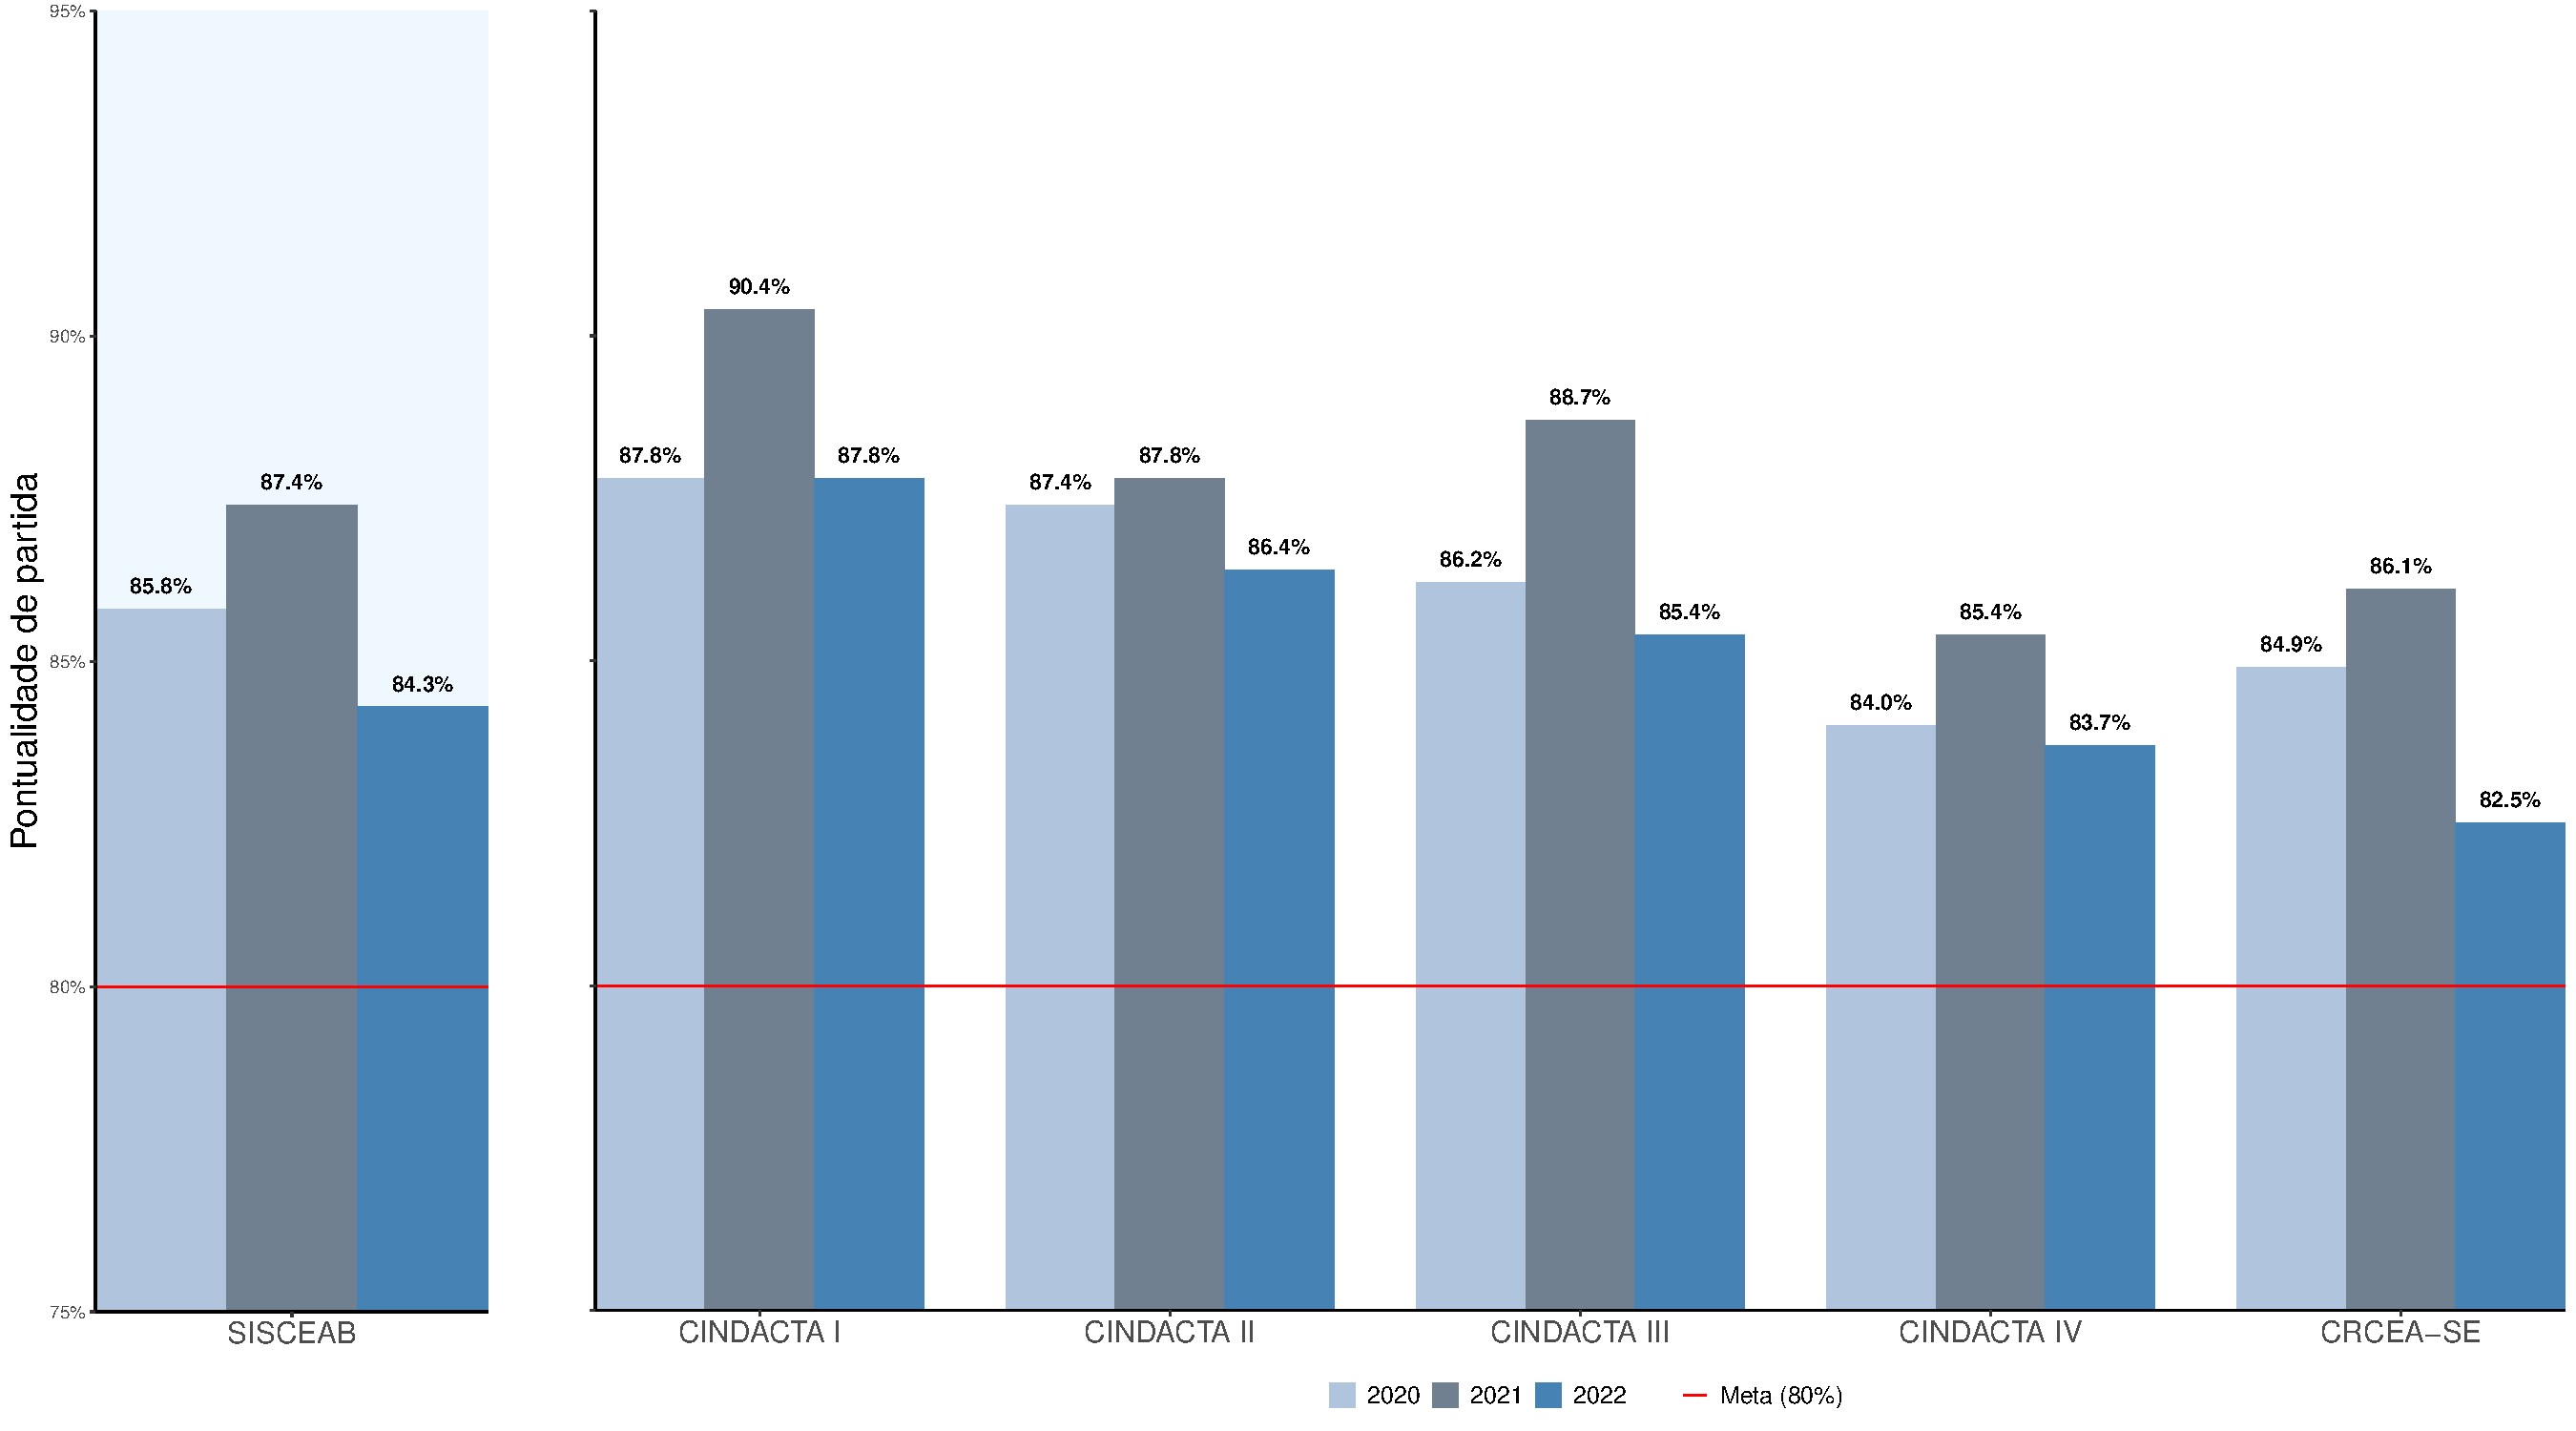
\includegraphics{_main_files/figure-latex/unnamed-chunk-11-1.pdf}

\#6 MAPA DE DENSIDADE

\begin{verbatim}
##   |                                                                              |                                                                      |   0%  |                                                                              |===                                                                   |   4%  |                                                                              |=====                                                                 |   7%  |                                                                              |========                                                              |  11%  |                                                                              |==========                                                            |  15%  |                                                                              |=============                                                         |  19%  |                                                                              |================                                                      |  22%  |                                                                              |==================                                                    |  26%  |                                                                              |=====================                                                 |  30%  |                                                                              |=======================                                               |  33%  |                                                                              |==========================                                            |  37%  |                                                                              |=============================                                         |  41%  |                                                                              |===============================                                       |  44%  |                                                                              |==================================                                    |  48%  |                                                                              |====================================                                  |  52%  |                                                                              |=======================================                               |  56%  |                                                                              |=========================================                             |  59%  |                                                                              |============================================                          |  63%  |                                                                              |===============================================                       |  67%  |                                                                              |=================================================                     |  70%  |                                                                              |====================================================                  |  74%  |                                                                              |======================================================                |  78%  |                                                                              |=========================================================             |  81%  |                                                                              |============================================================          |  85%  |                                                                              |==============================================================        |  89%  |                                                                              |=================================================================     |  93%  |                                                                              |===================================================================   |  96%  |                                                                              |======================================================================| 100%
\end{verbatim}

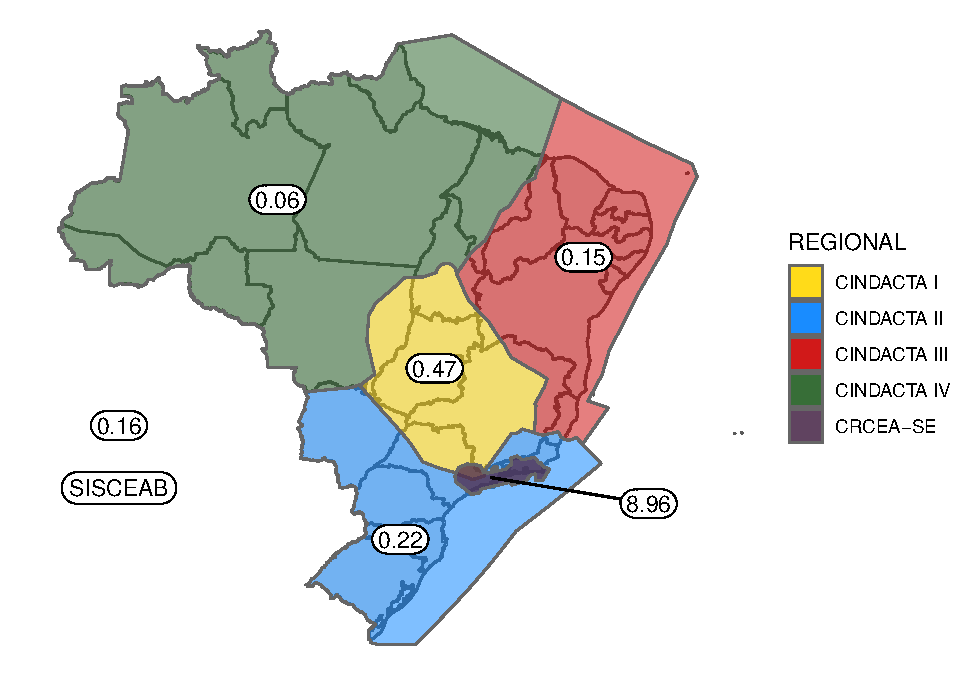
\includegraphics{_main_files/figure-latex/unnamed-chunk-12-1.pdf}

\#7 PONTUALIDADE DE PARTIDA

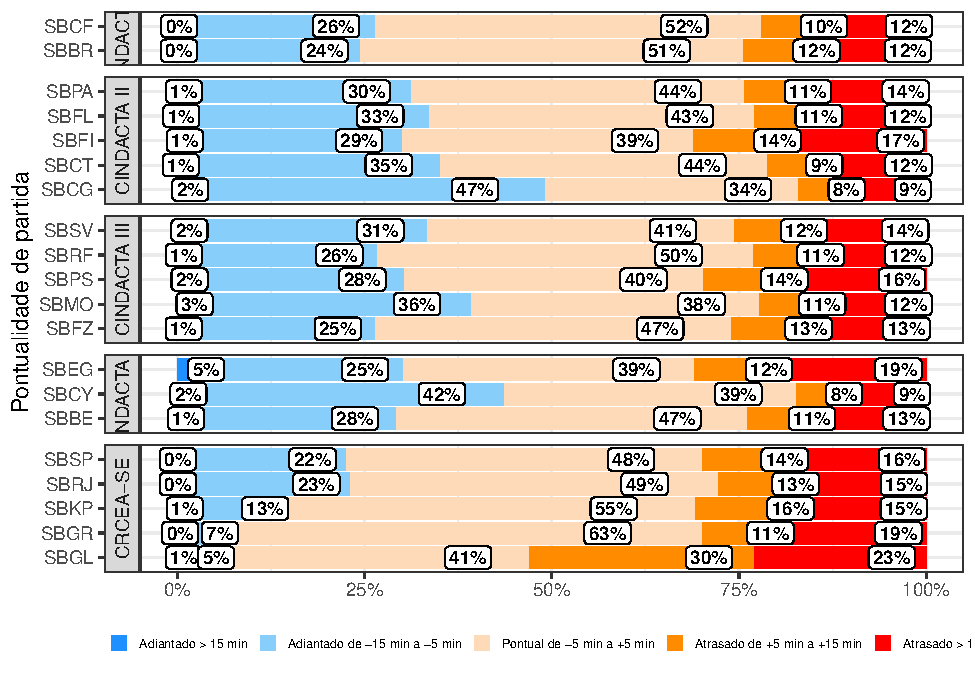
\includegraphics{_main_files/figure-latex/unnamed-chunk-13-1.pdf}

\#\#7A PONTUALIDADE DE PARTIDA

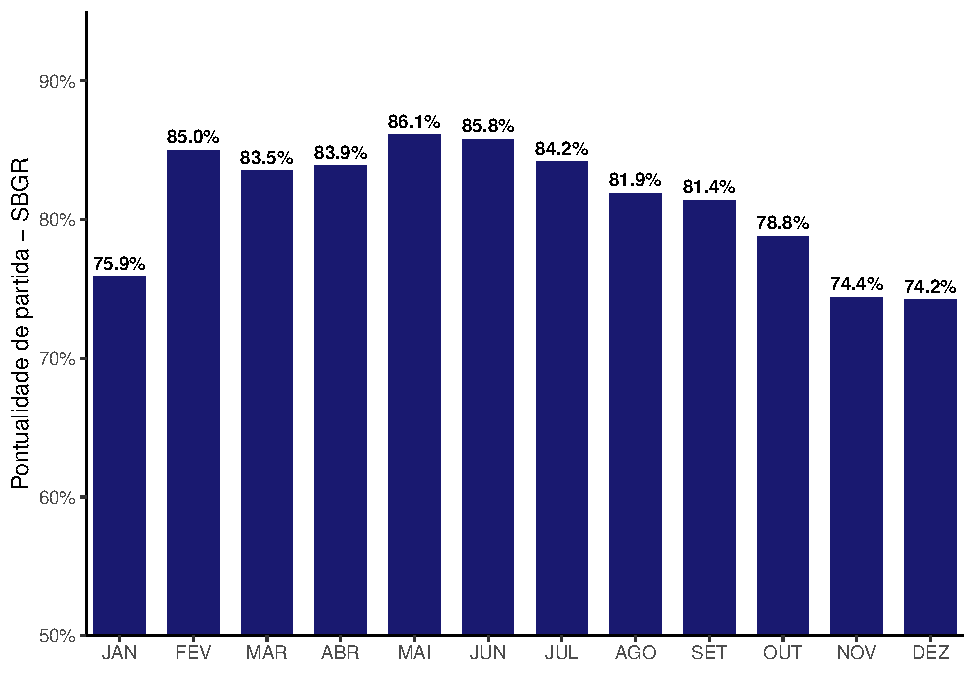
\includegraphics{_main_files/figure-latex/unnamed-chunk-14-1.pdf} 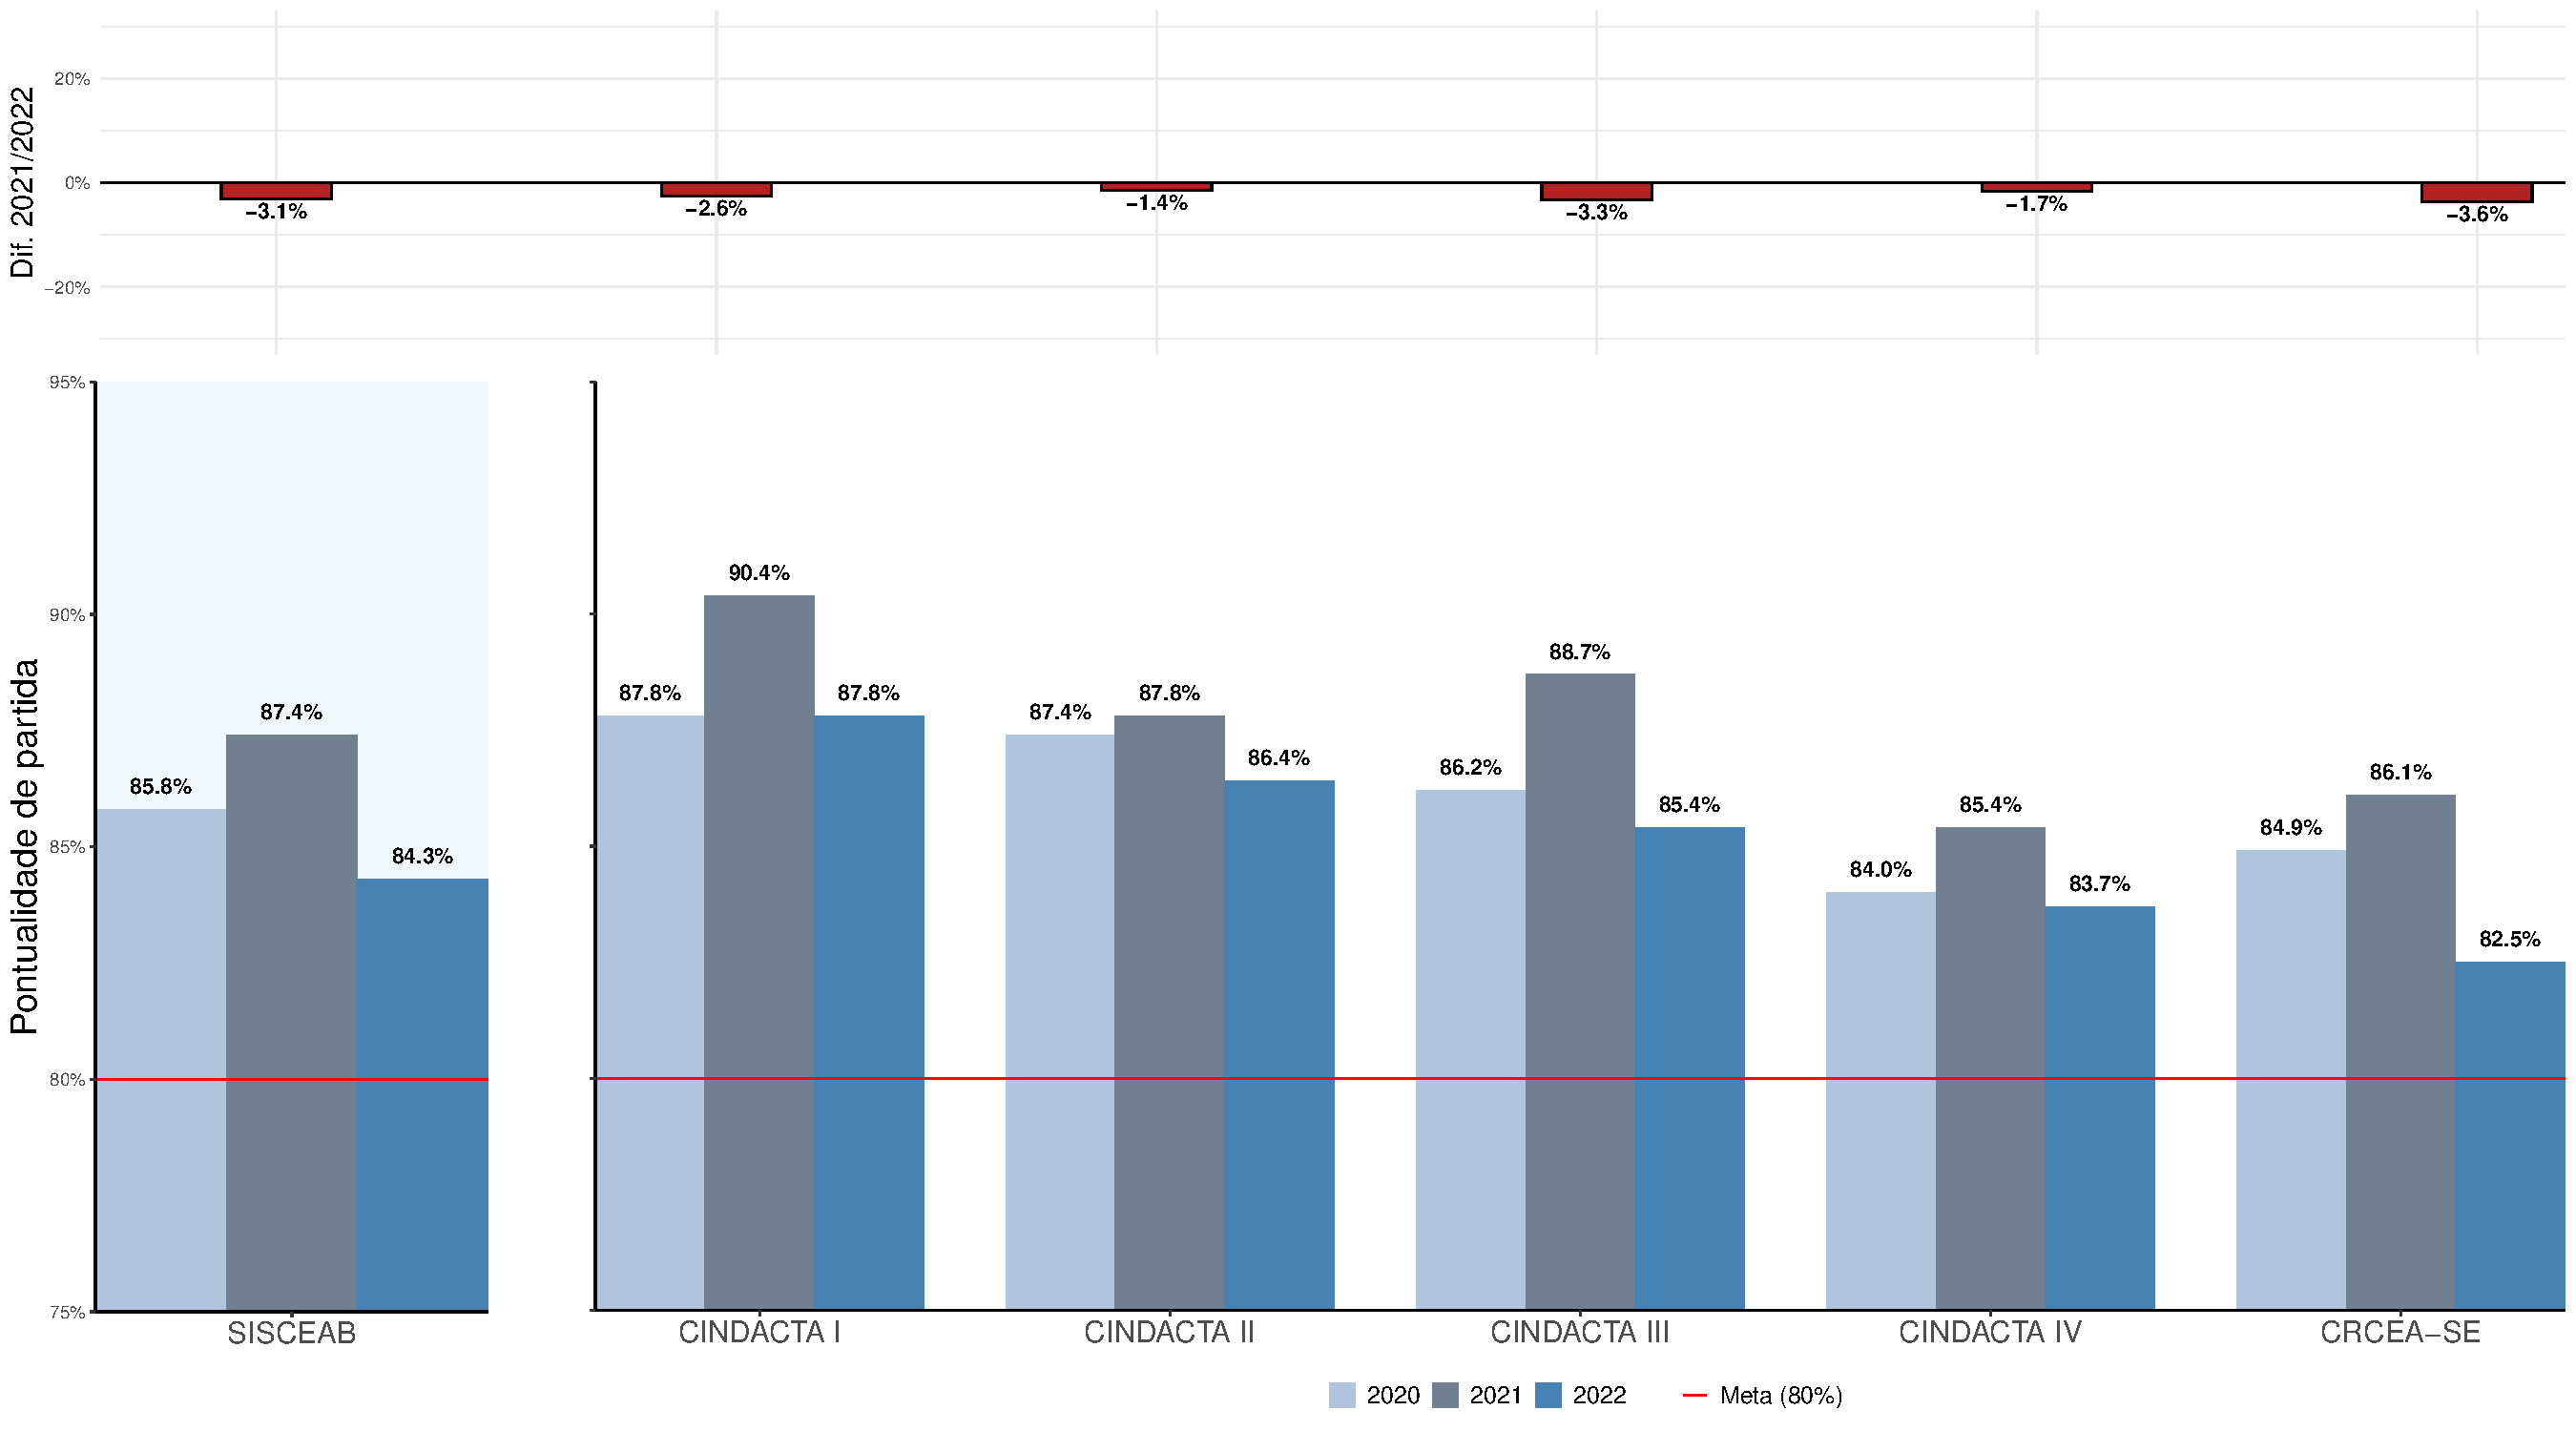
\includegraphics{_main_files/figure-latex/unnamed-chunk-14-2.pdf}

\#8 PONTUALIDADE DE CHEGADA

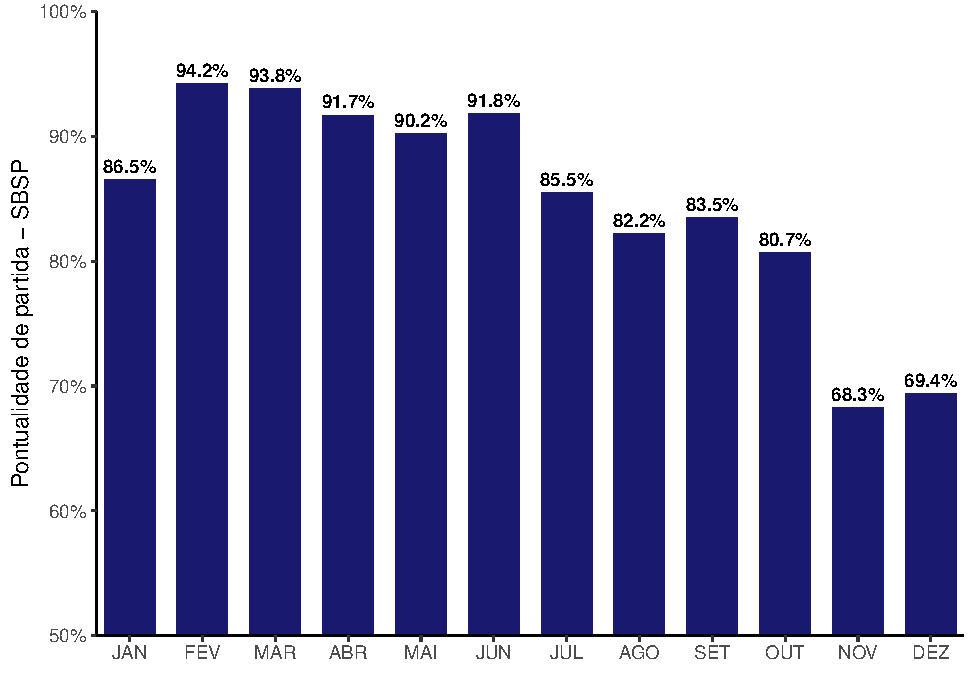
\includegraphics{_main_files/figure-latex/unnamed-chunk-15-1.pdf}

\#\#8.1 PONTUALIDADE DE CHEGADA

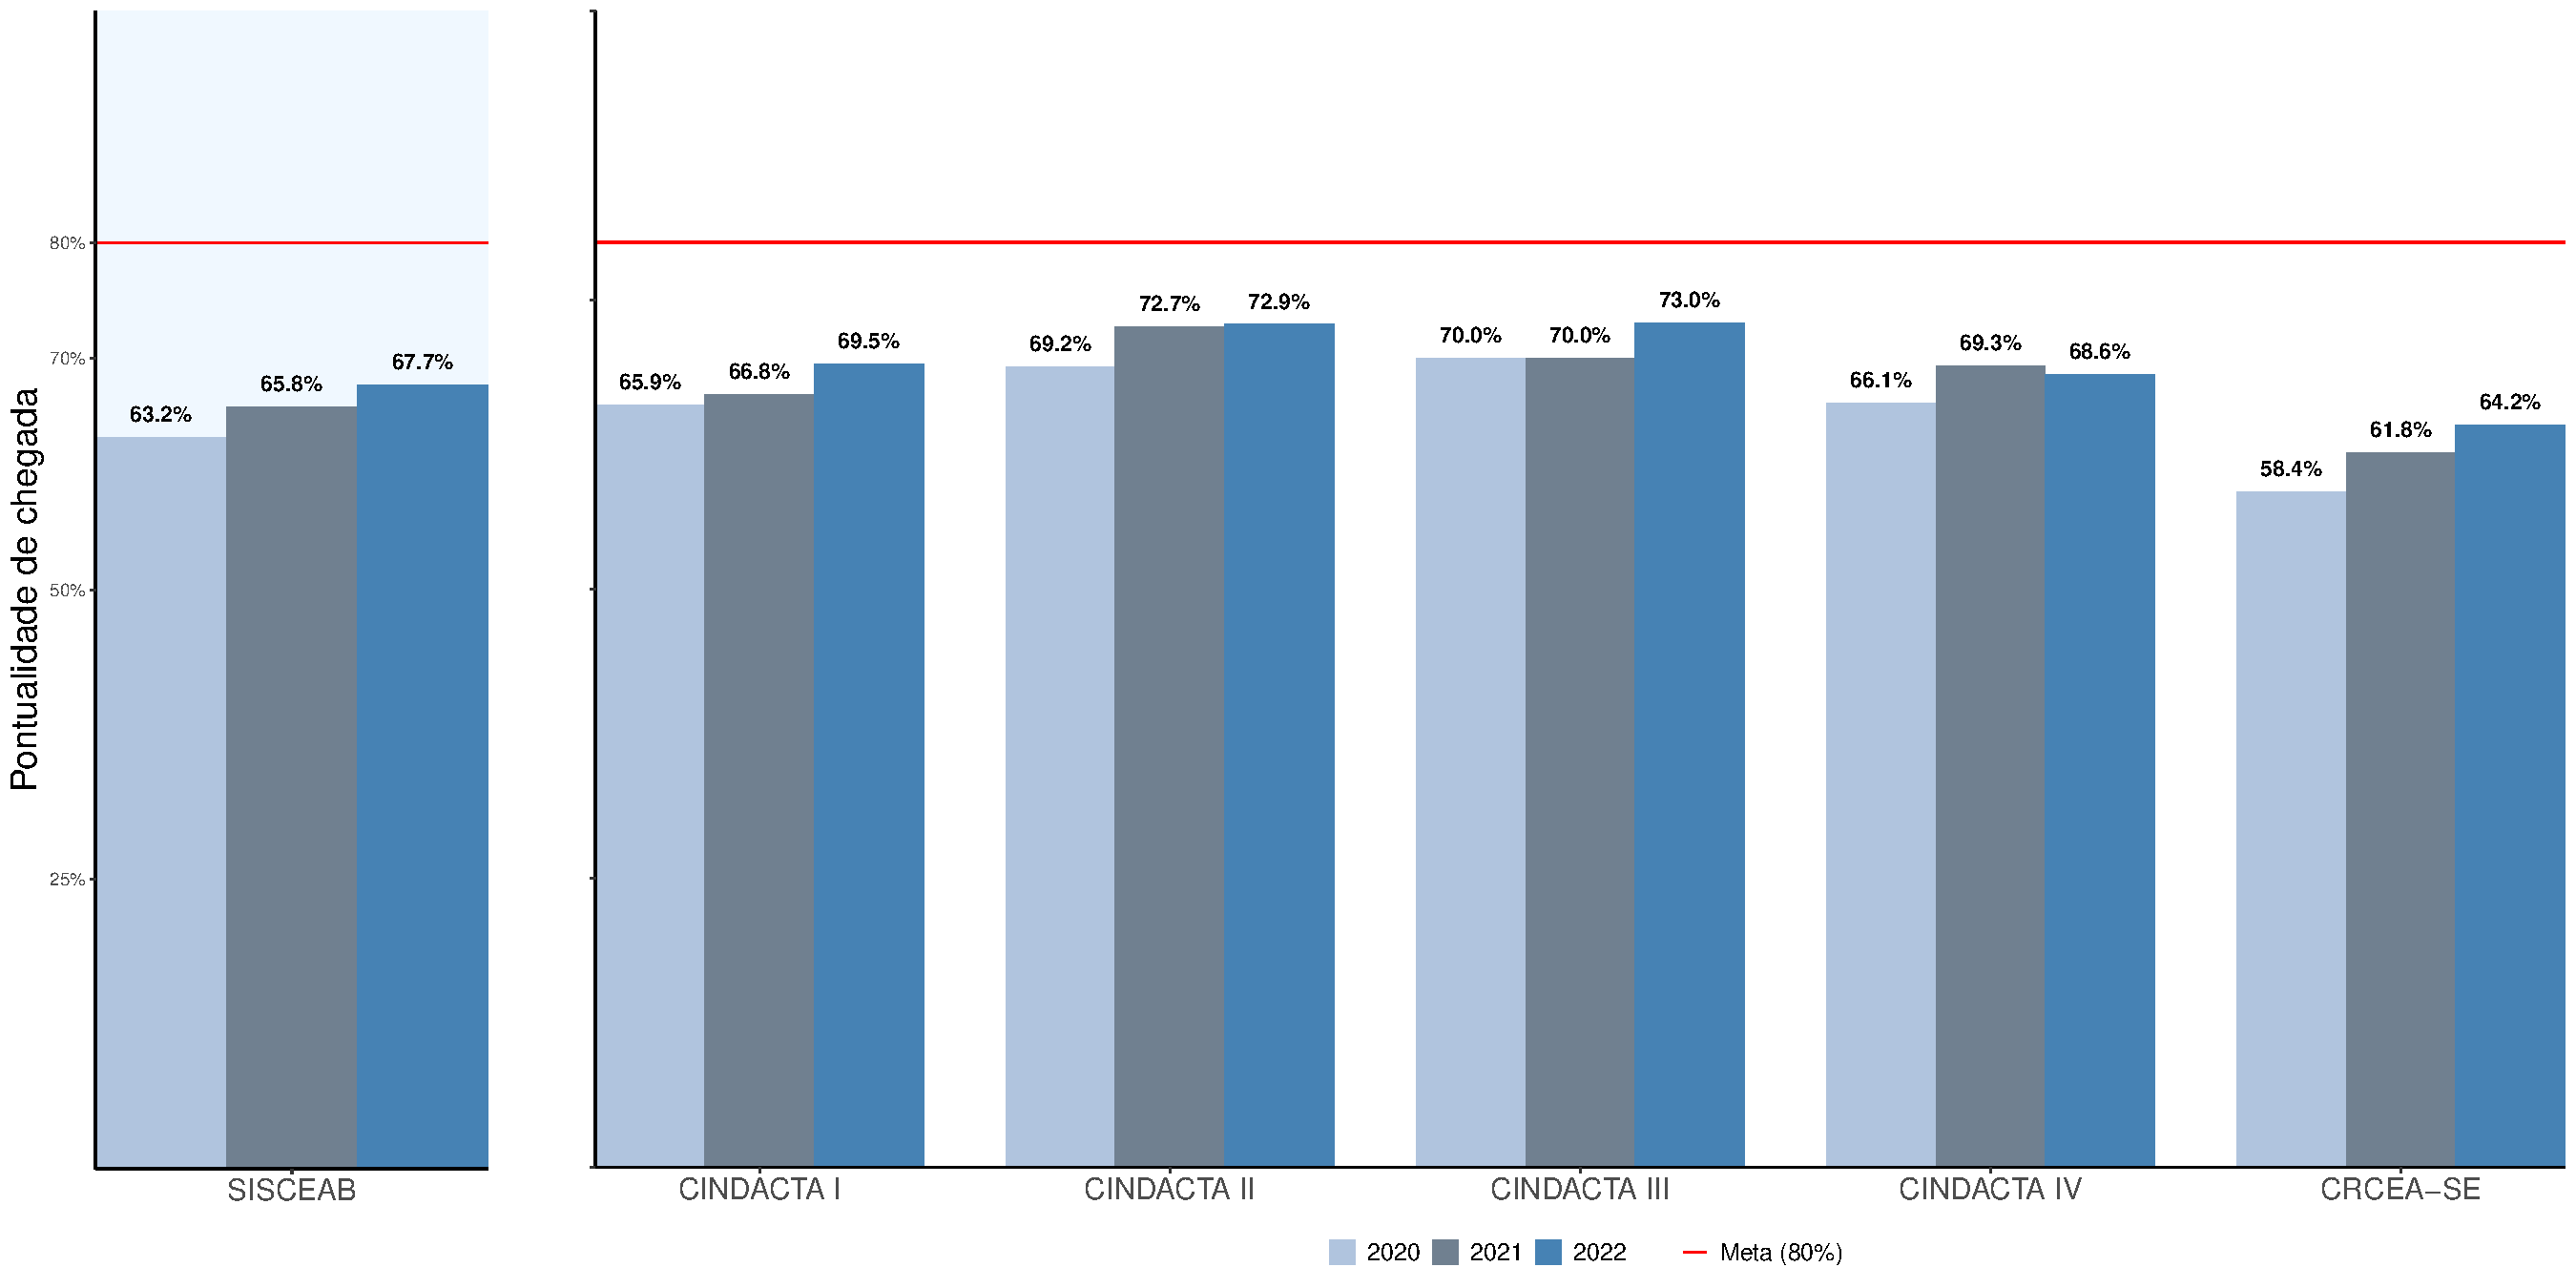
\includegraphics{_main_files/figure-latex/unnamed-chunk-16-1.pdf} 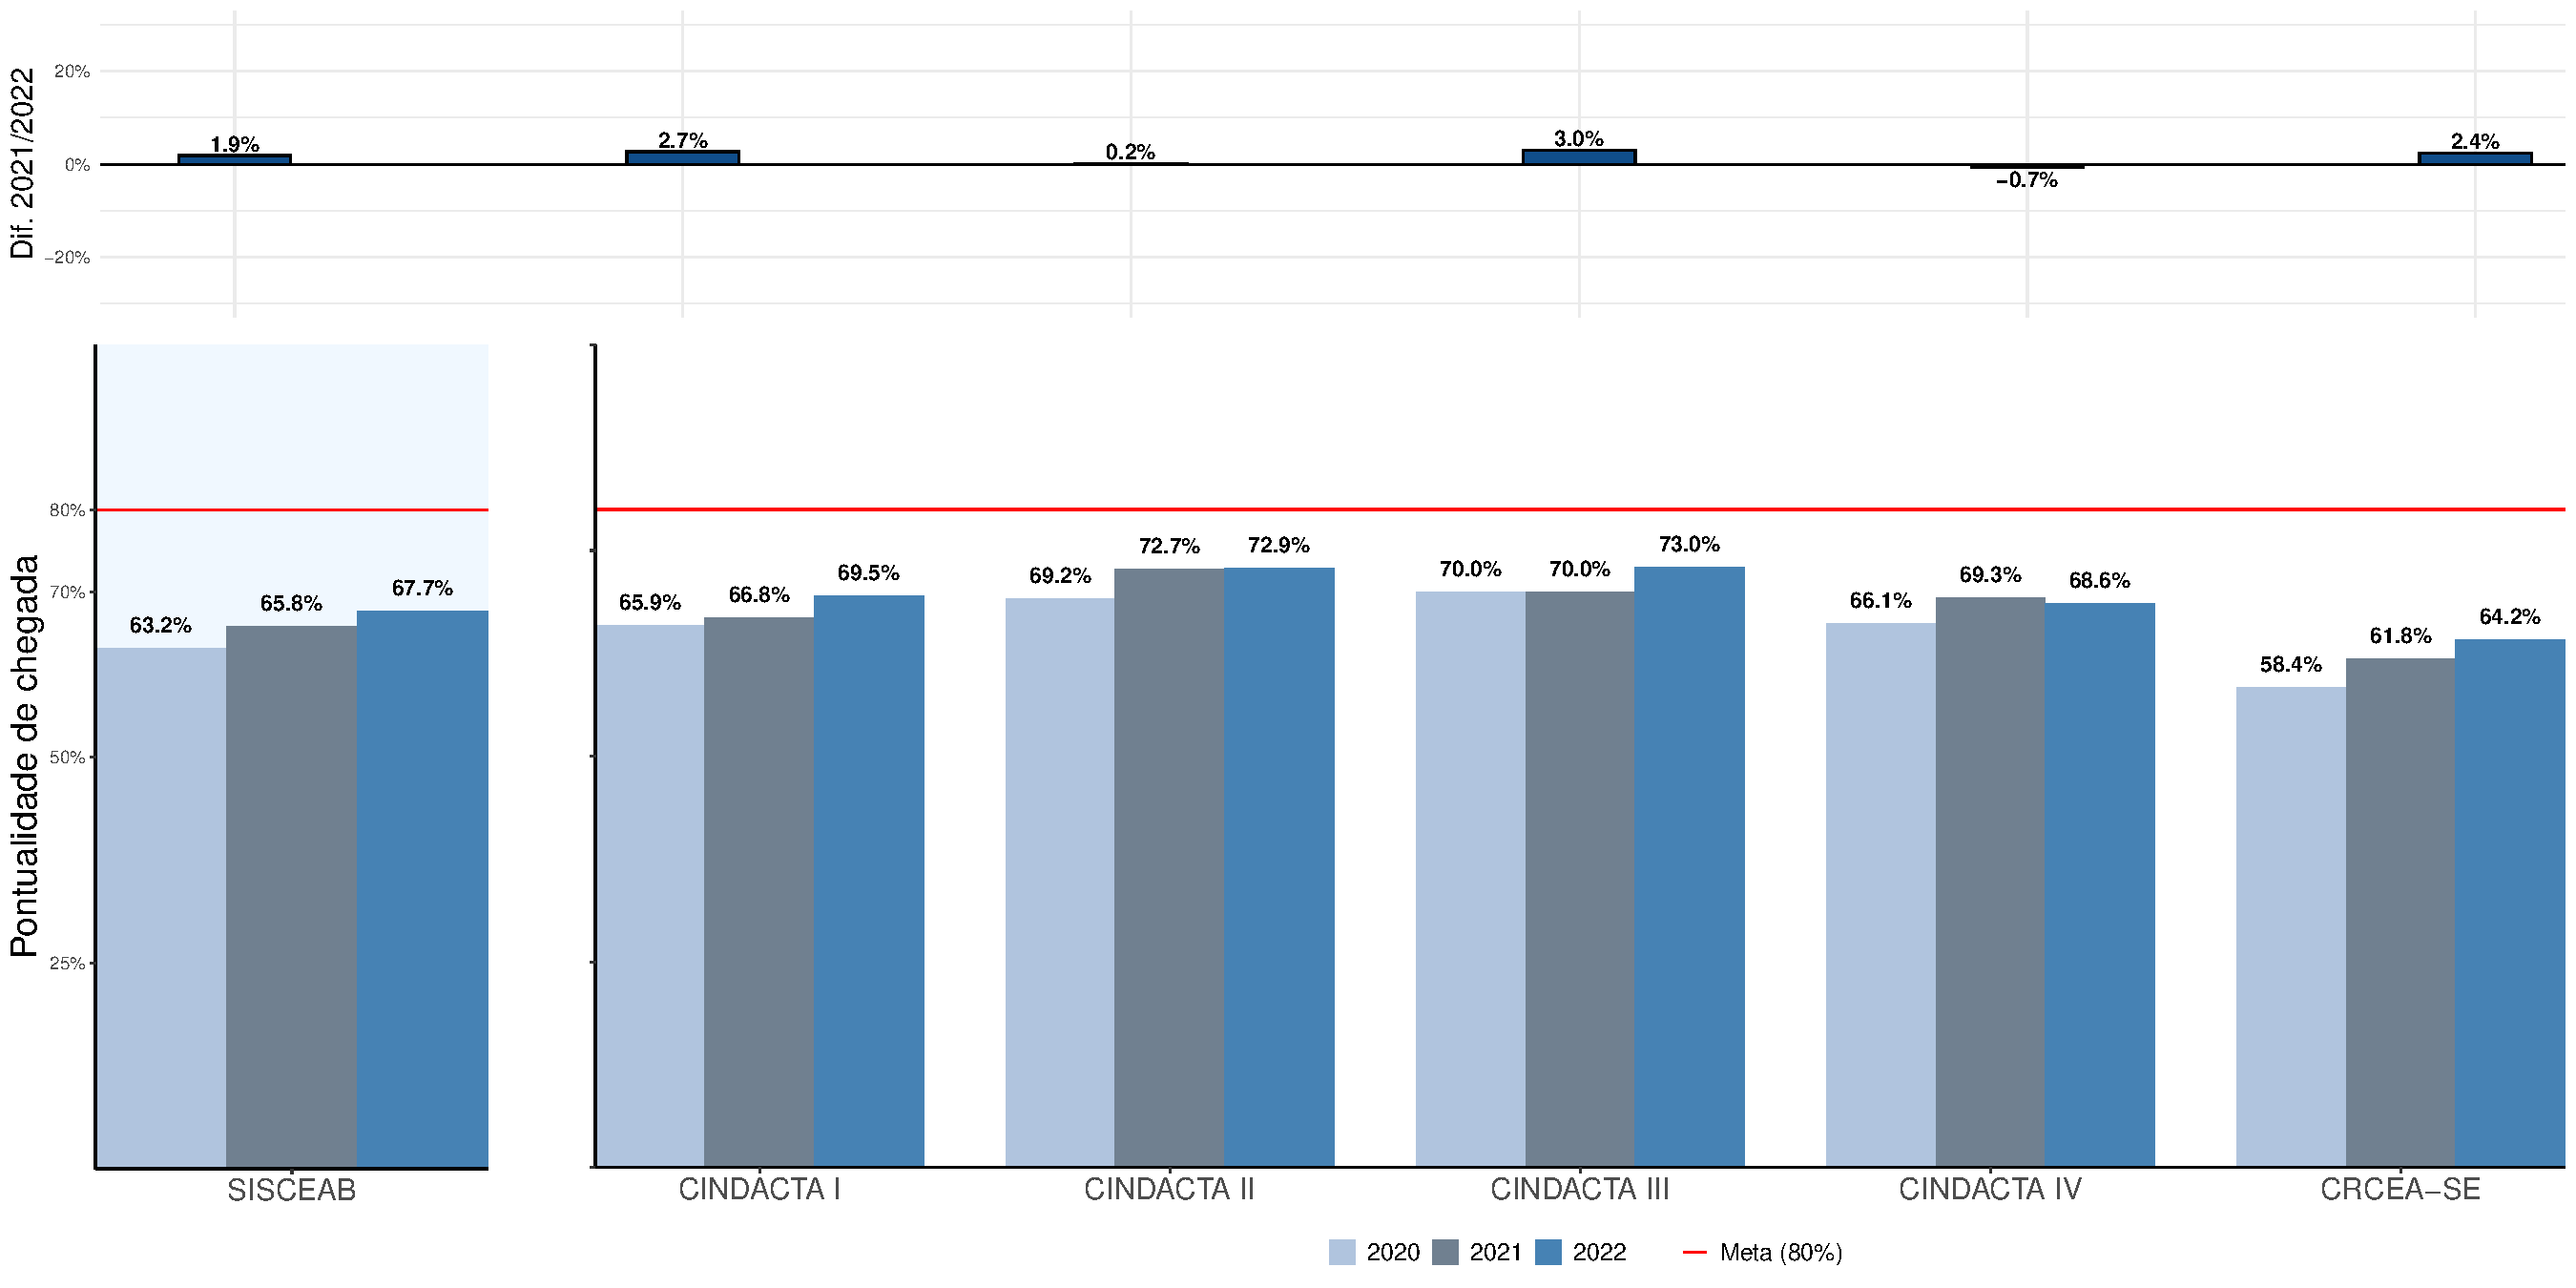
\includegraphics{_main_files/figure-latex/unnamed-chunk-16-2.pdf}

\hypertarget{dep-e-arr}{%
\section{8.2 DEP e ARR}\label{dep-e-arr}}

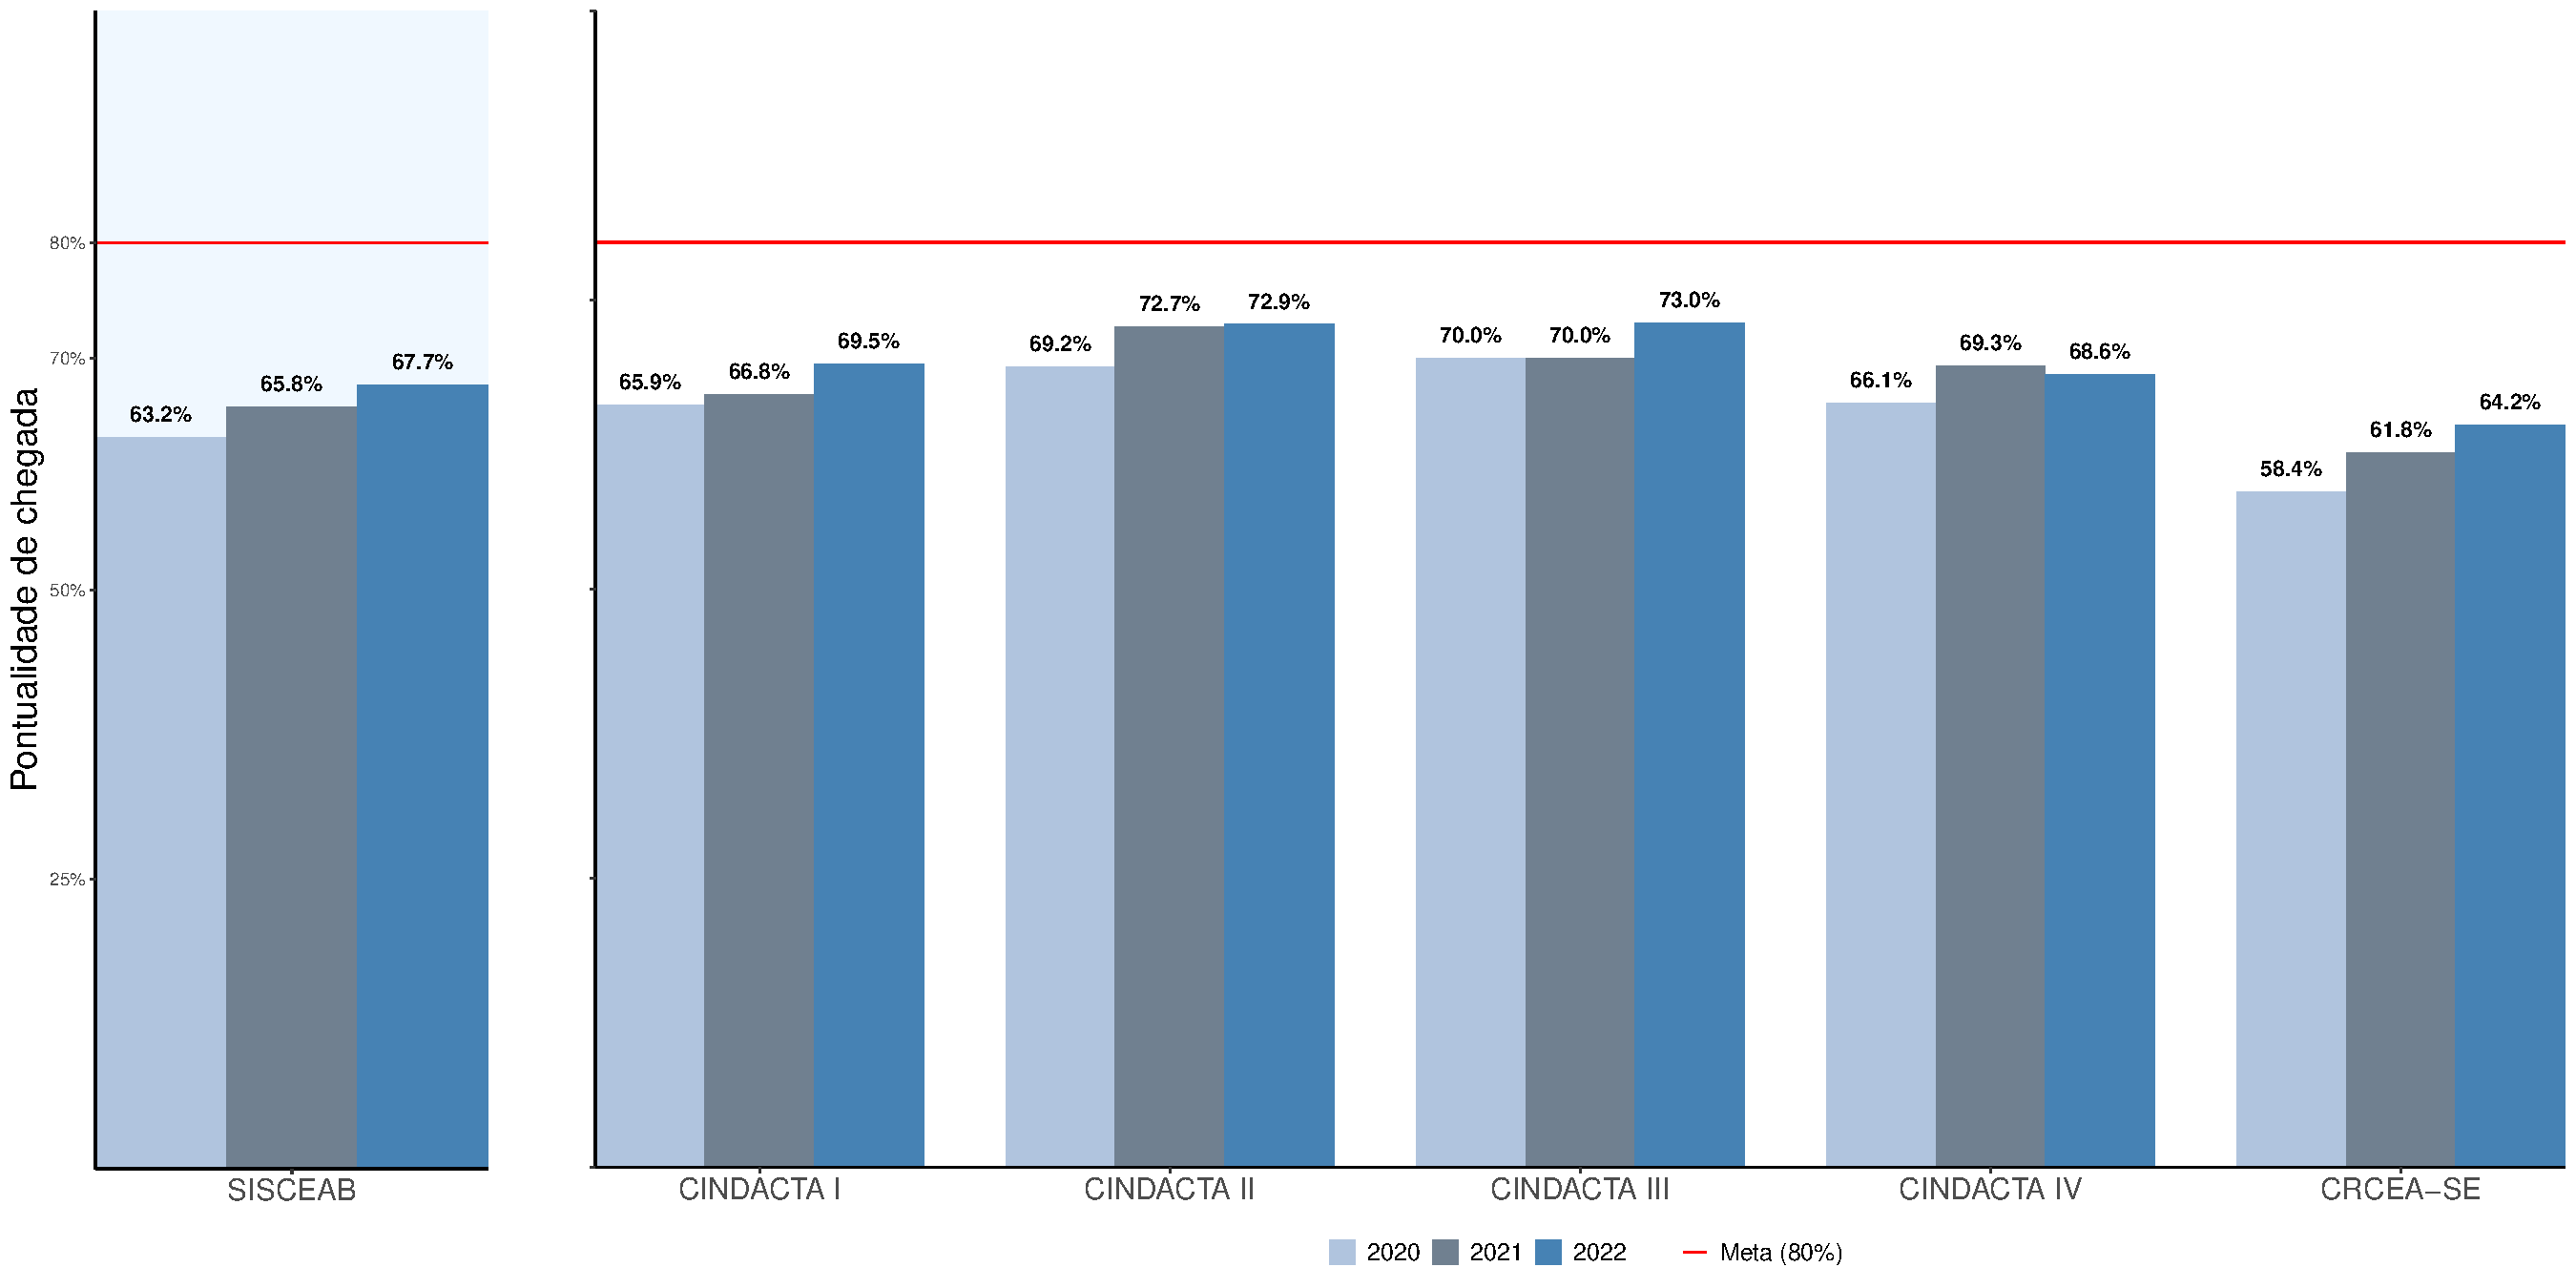
\includegraphics{_main_files/figure-latex/unnamed-chunk-17-1.pdf}

\#9 PONTUALIDADE DE PARTIDA SBGR

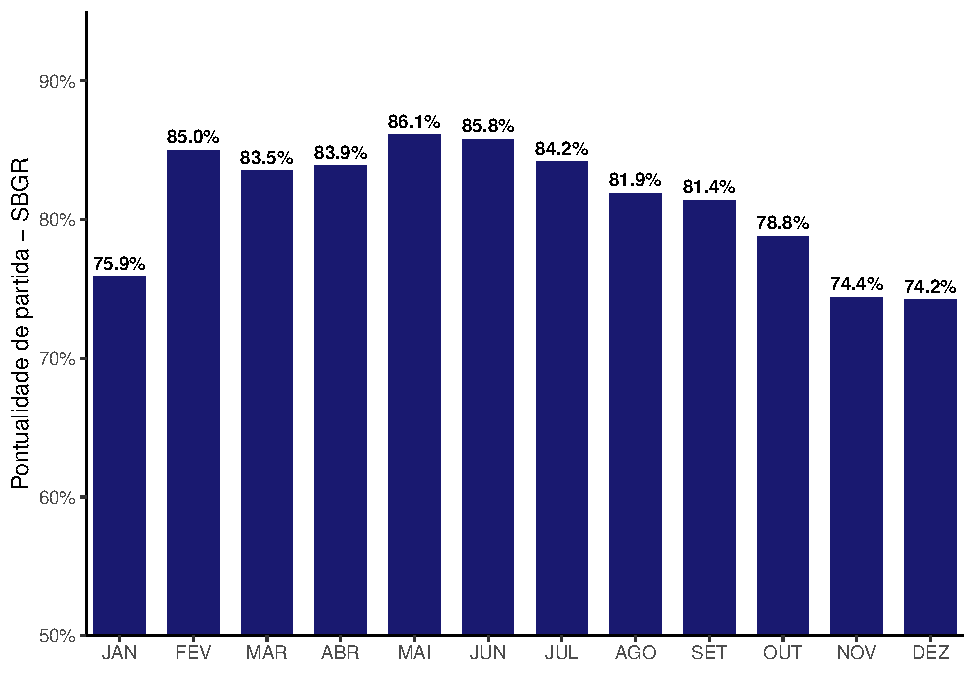
\includegraphics{_main_files/figure-latex/unnamed-chunk-18-1.pdf}

\#10 PONTUALIDADE DE PARTIDA SBSP

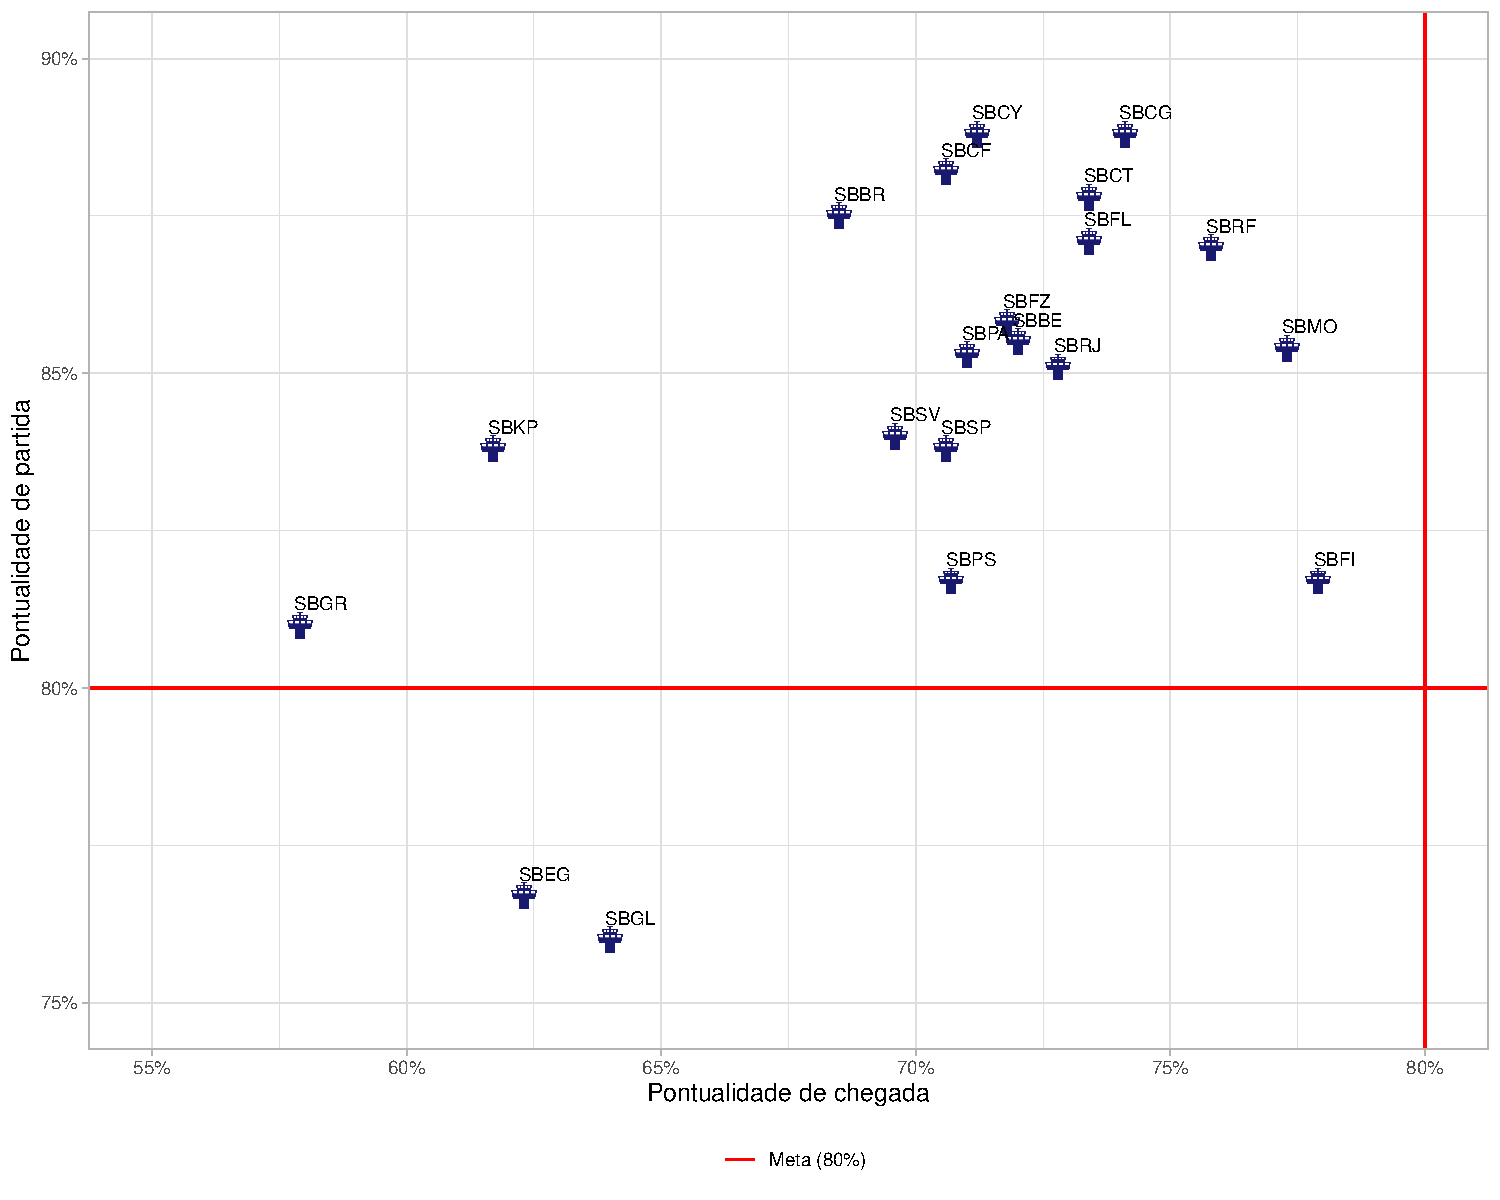
\includegraphics{_main_files/figure-latex/unnamed-chunk-19-1.pdf}

\#11 PONTUALIDADE DE CHEGADA SBGR

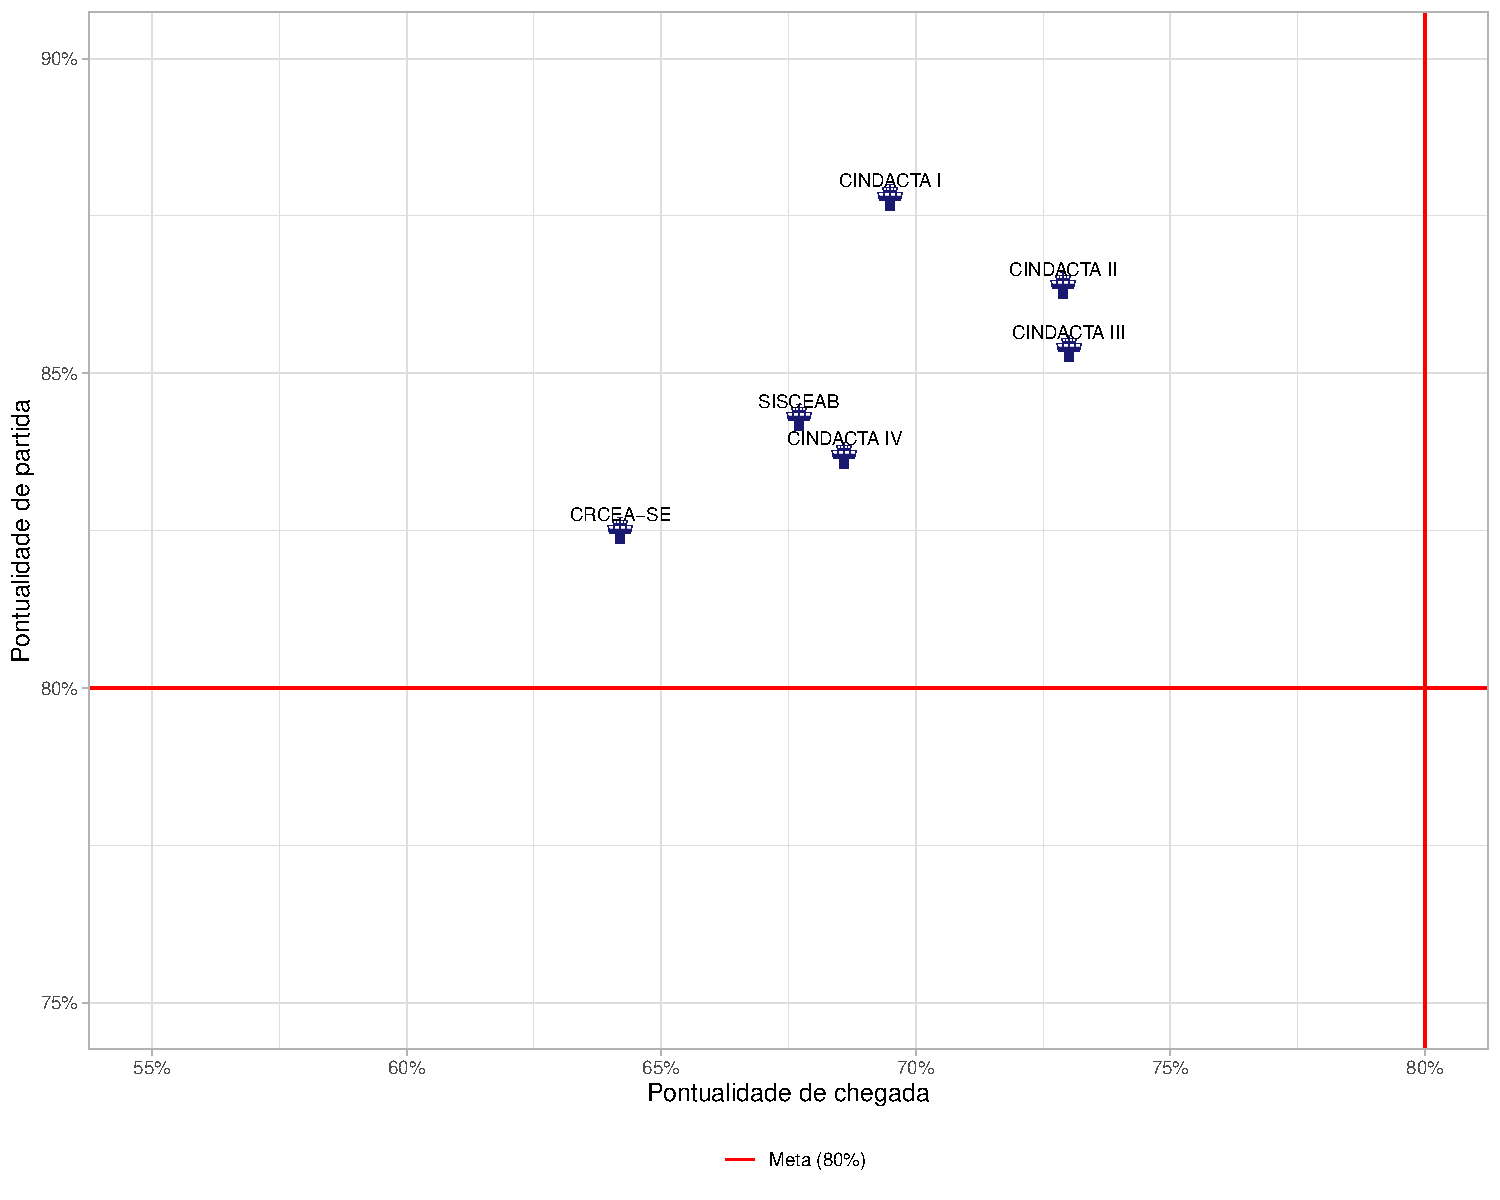
\includegraphics{_main_files/figure-latex/unnamed-chunk-20-1.pdf}

\#\#11.1 PONTUALIDADE DE CHEGADA SBSP

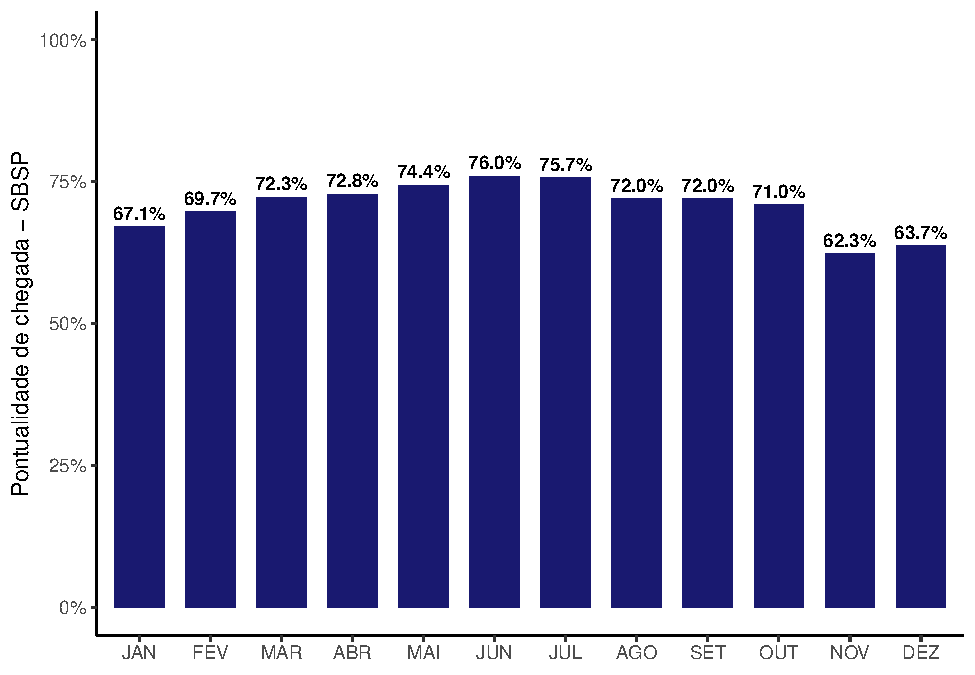
\includegraphics{_main_files/figure-latex/unnamed-chunk-21-1.pdf}

\#12 Pontualidade ARR em 2022

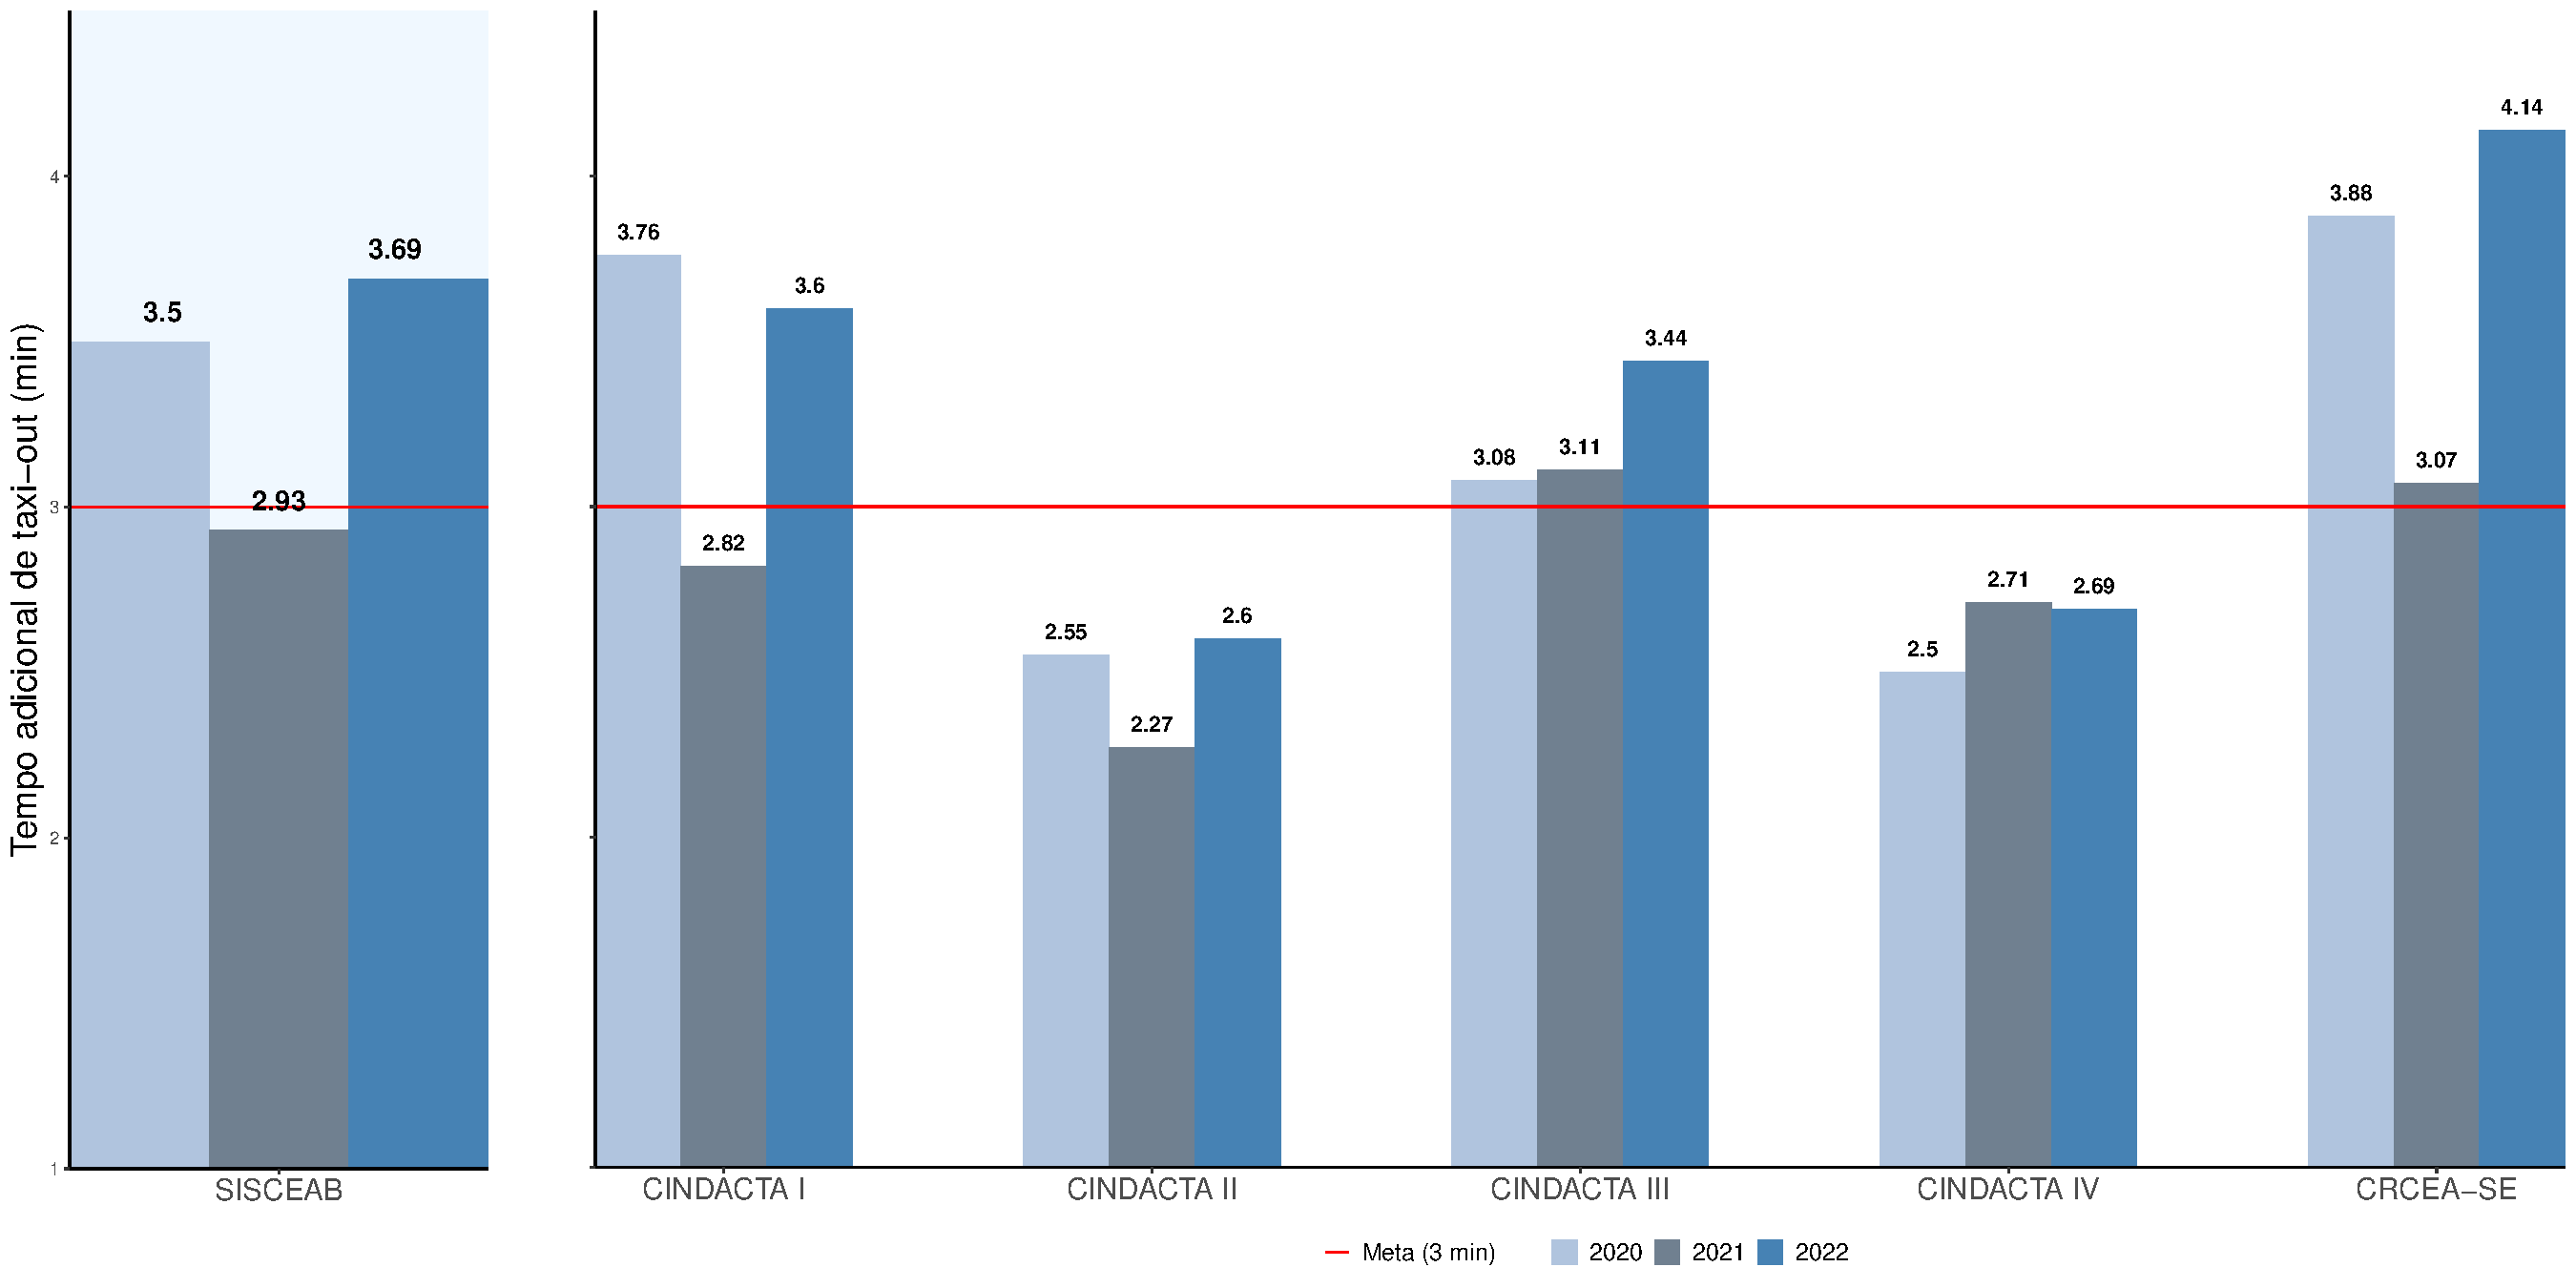
\includegraphics{_main_files/figure-latex/unnamed-chunk-22-1.pdf}

\hypertarget{pontualidade-dep-em-2022}{%
\chapter{13 Pontualidade DEP em 2022}\label{pontualidade-dep-em-2022}}

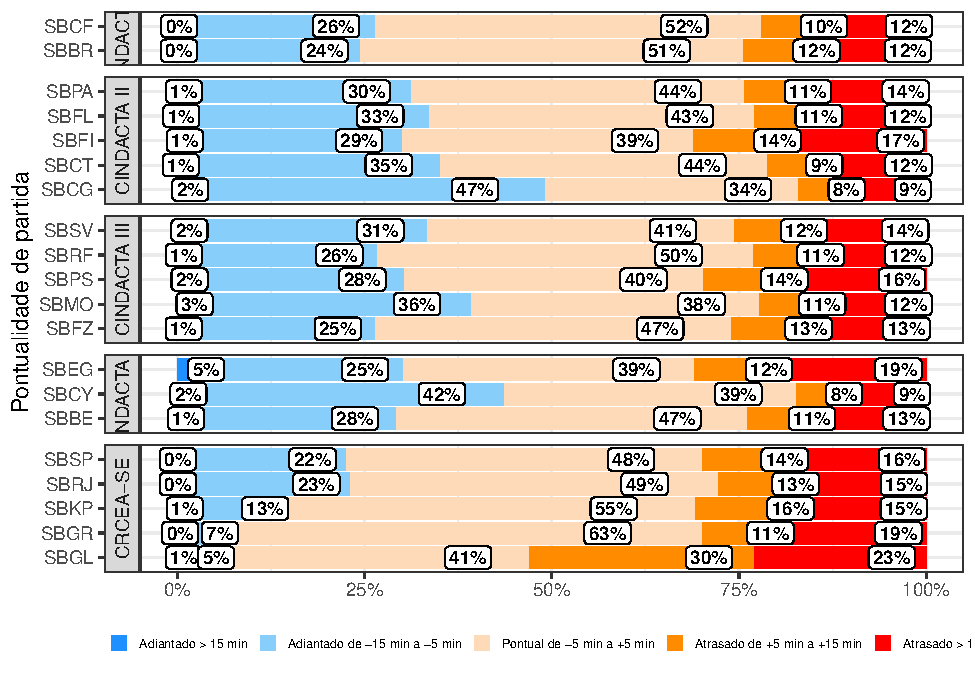
\includegraphics{_main_files/figure-latex/unnamed-chunk-23-1.pdf}

\hypertarget{muxe9dia-muxf3vel}{%
\chapter{14 MÉDIA MÓVEL}\label{muxe9dia-muxf3vel}}

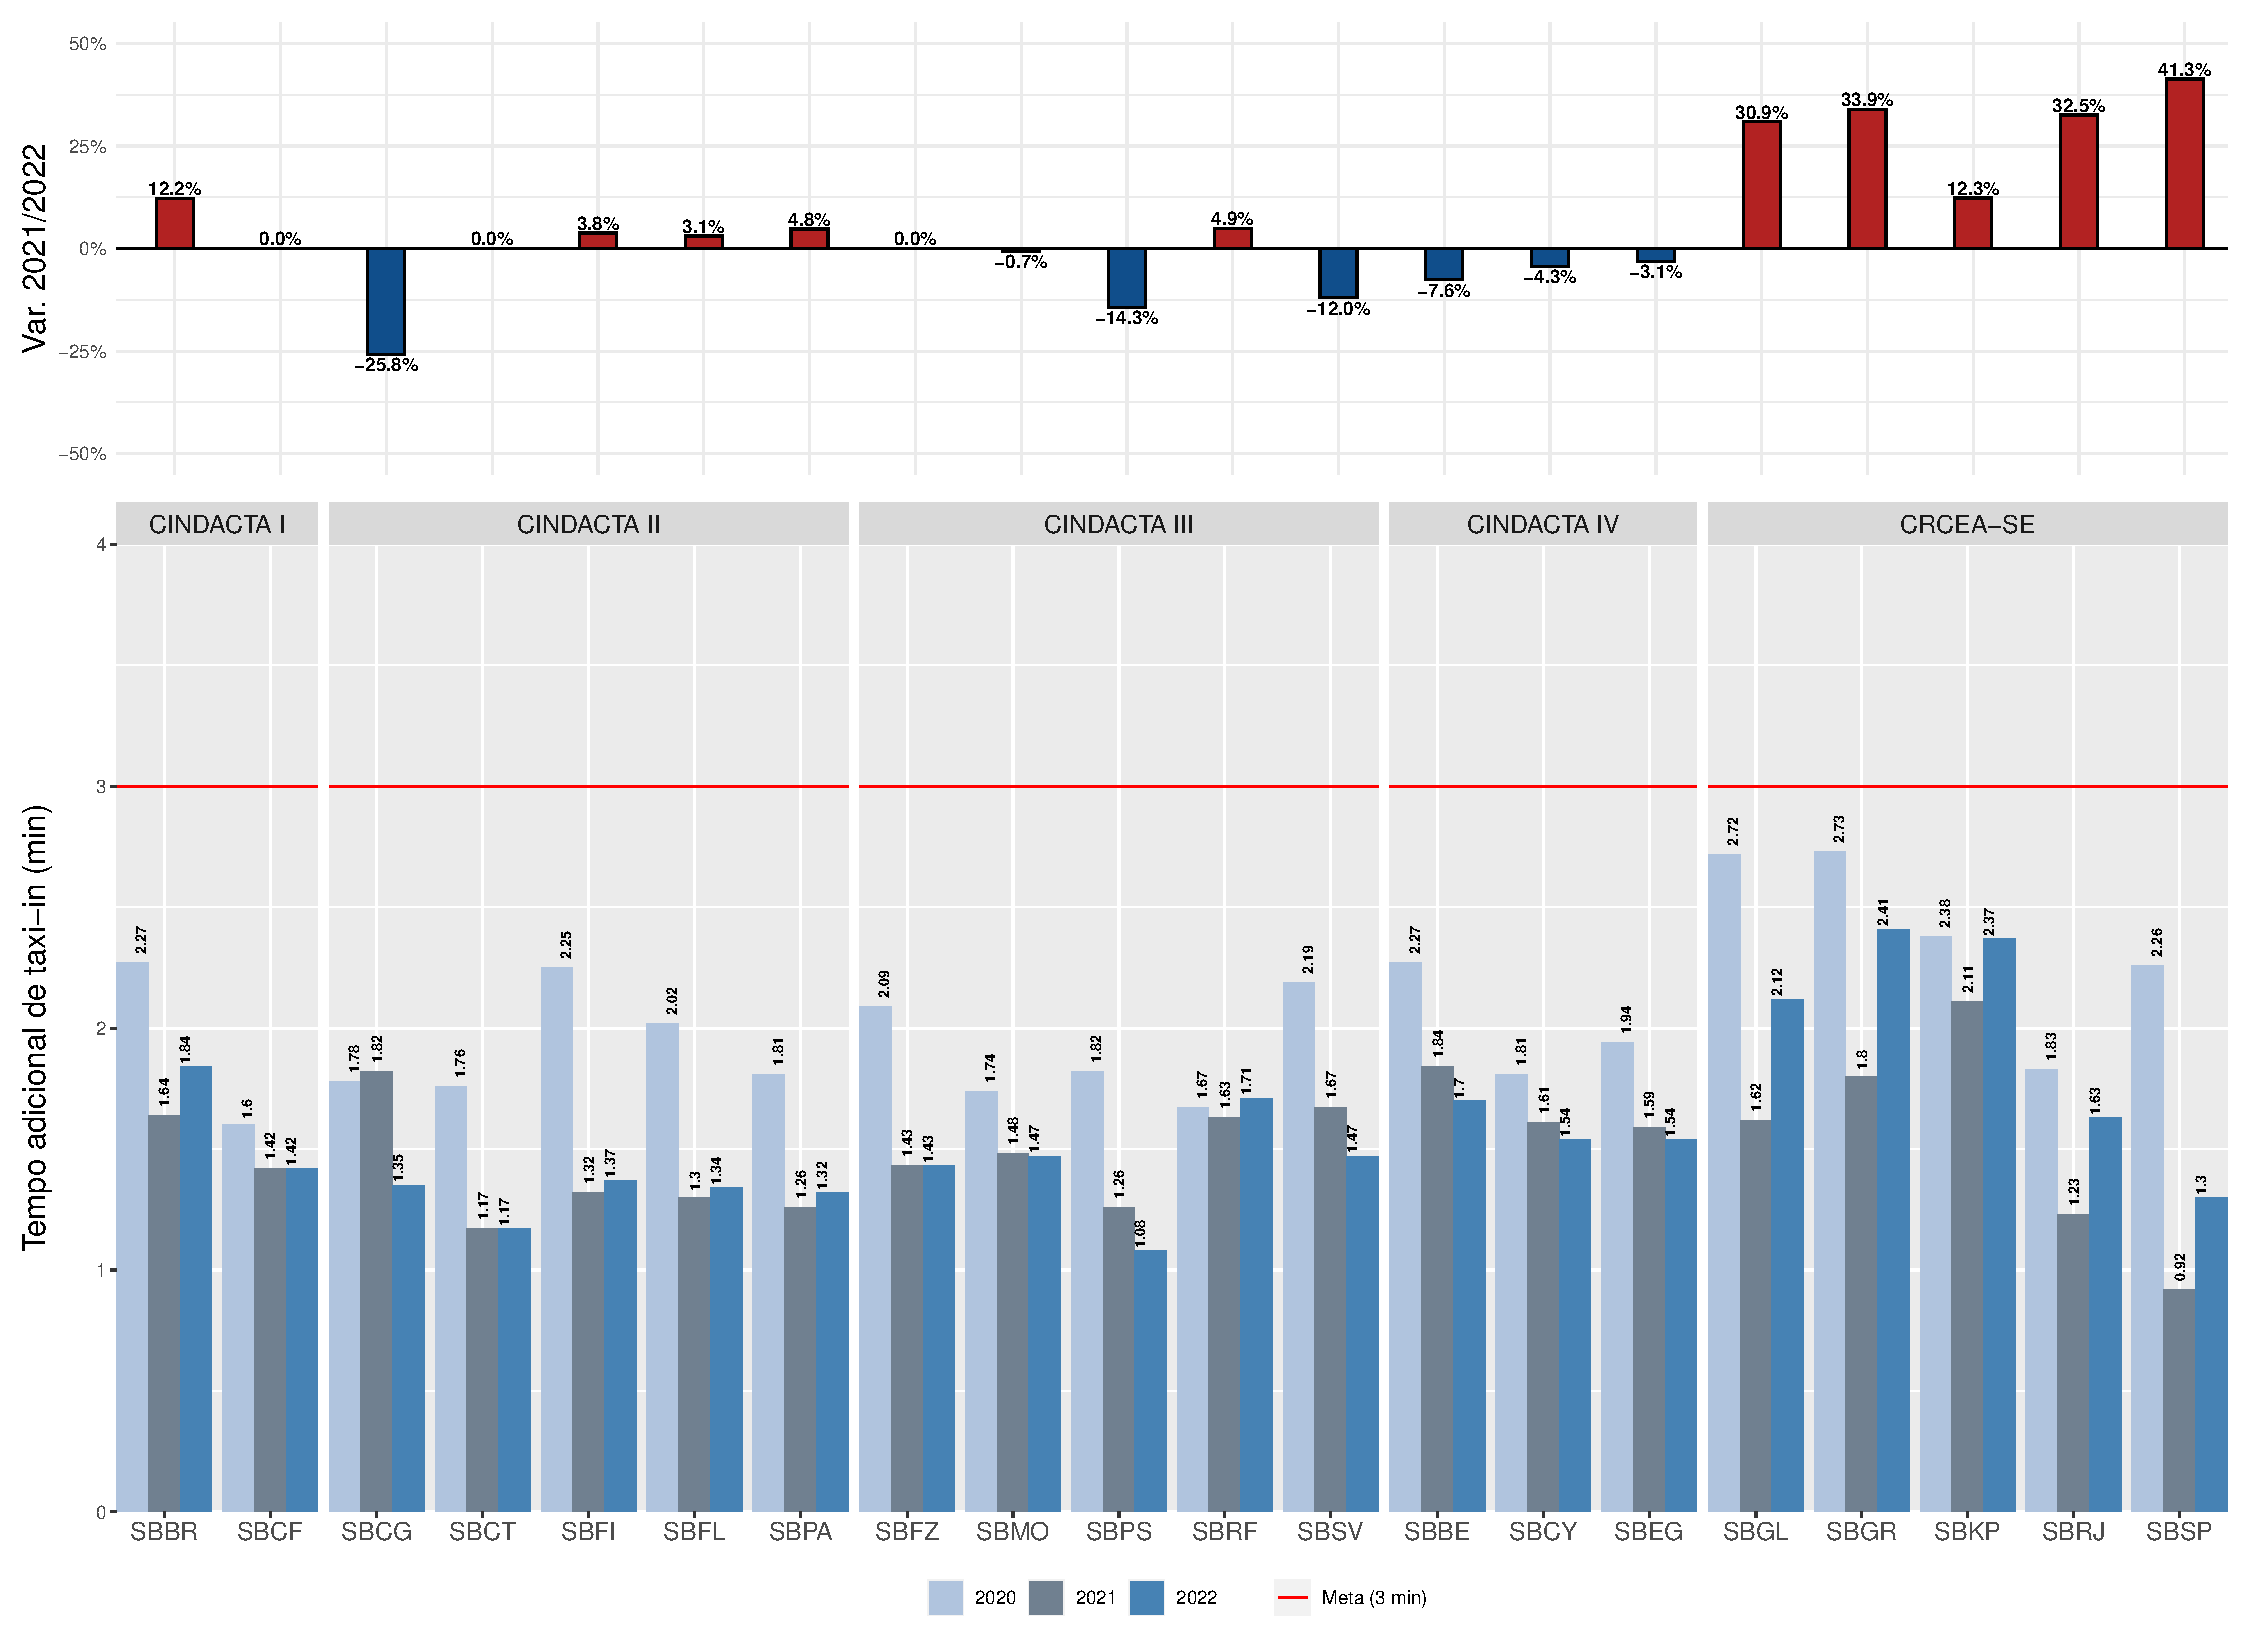
\includegraphics{_main_files/figure-latex/unnamed-chunk-24-1.pdf}

\hypertarget{dep-e-arr-regional}{%
\chapter{15 DEP e ARR REGIONAL}\label{dep-e-arr-regional}}

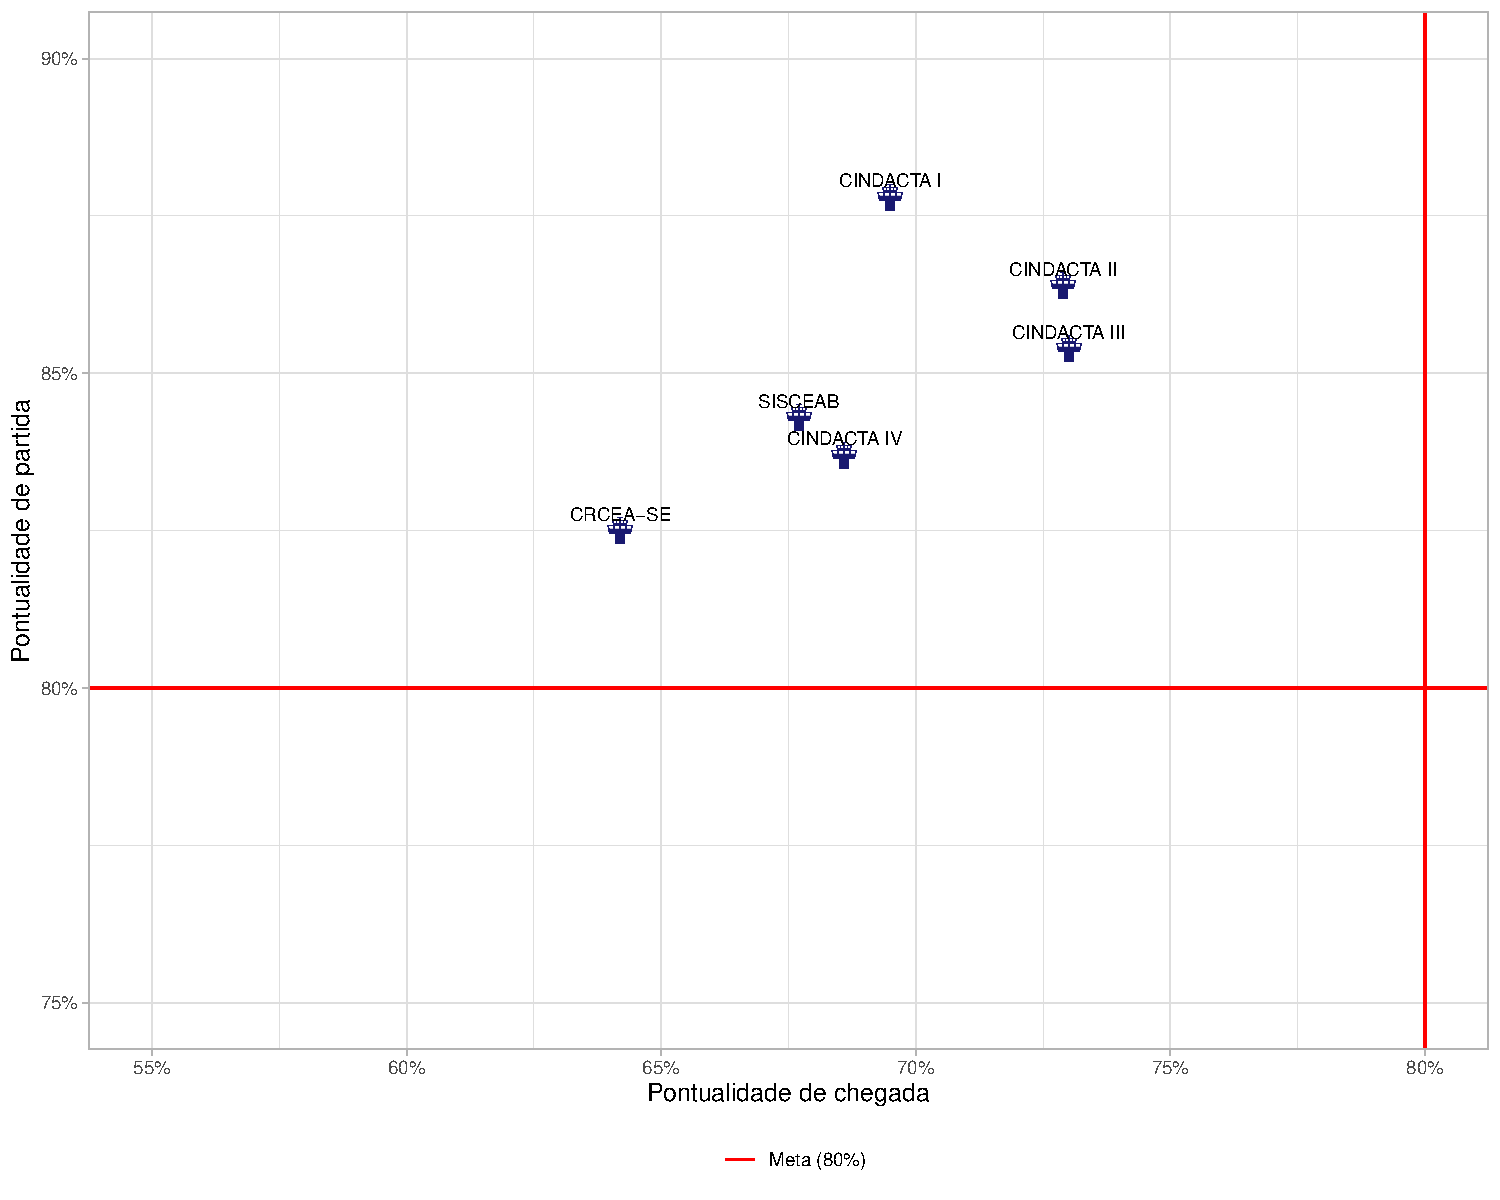
\includegraphics{_main_files/figure-latex/unnamed-chunk-25-1.pdf}

\#16 TAXIOUT

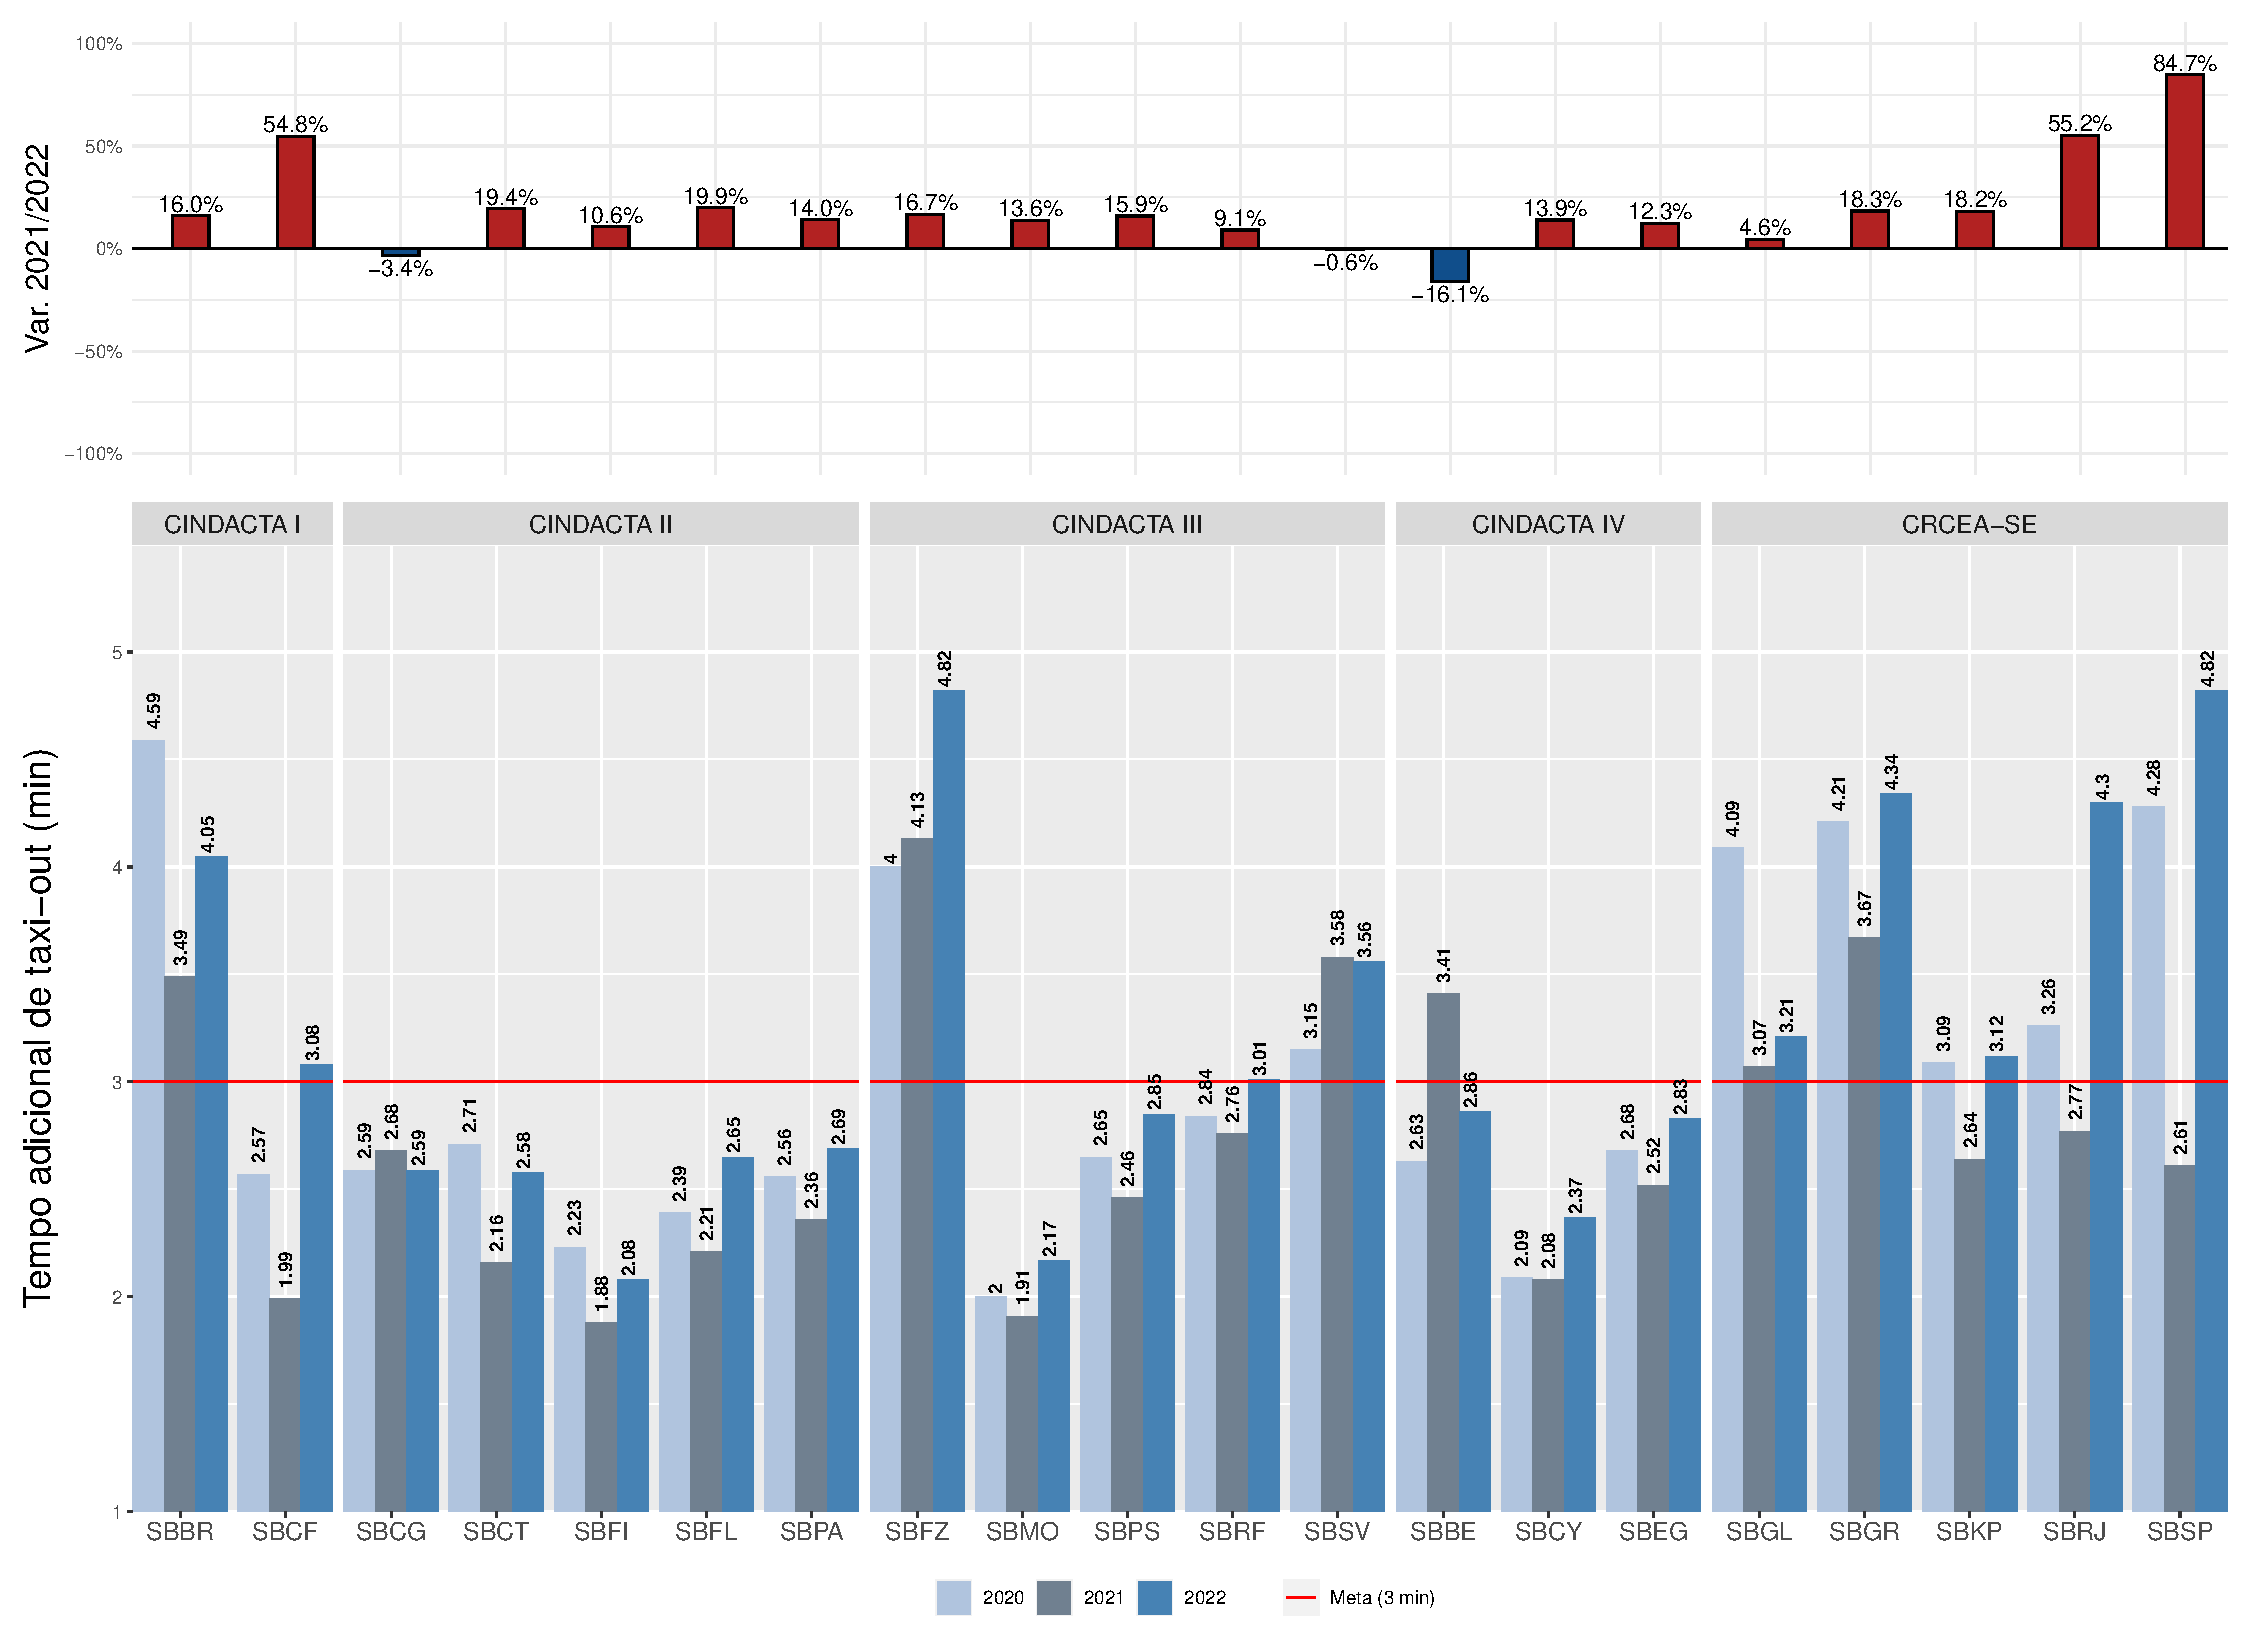
\includegraphics{_main_files/figure-latex/unnamed-chunk-26-1.pdf}

\#17 GRÁFICO DE TEMPO ADICIONAL DE TAXI-OUT POR REGIONAL

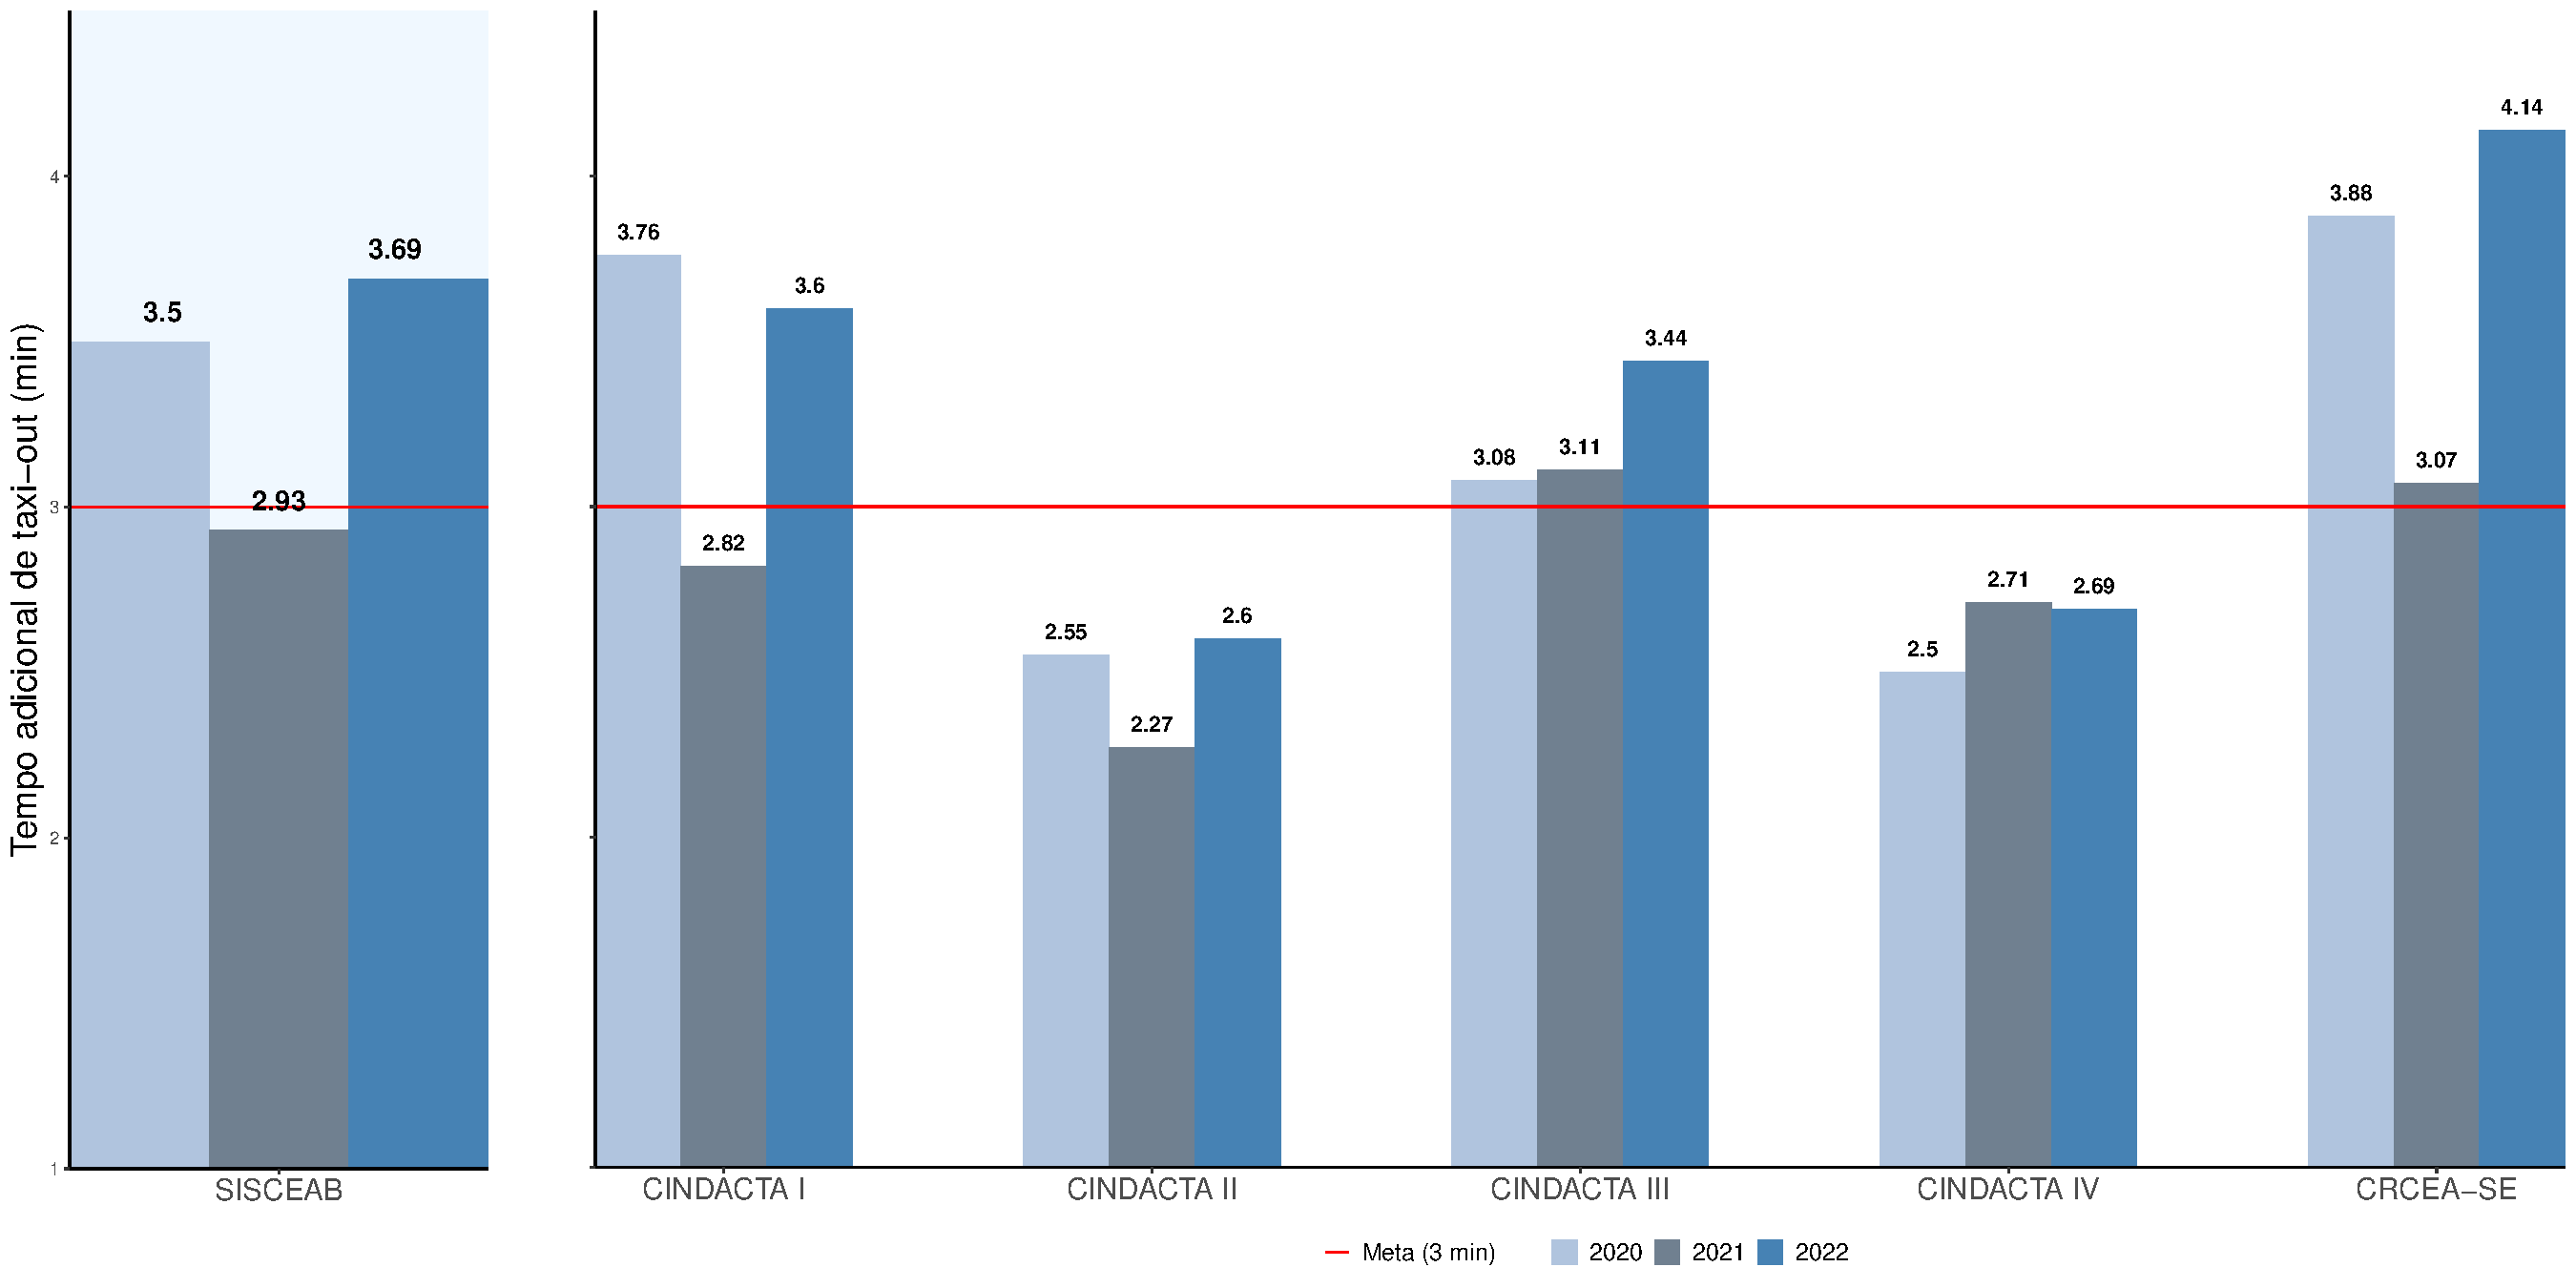
\includegraphics{_main_files/figure-latex/unnamed-chunk-27-1.pdf} 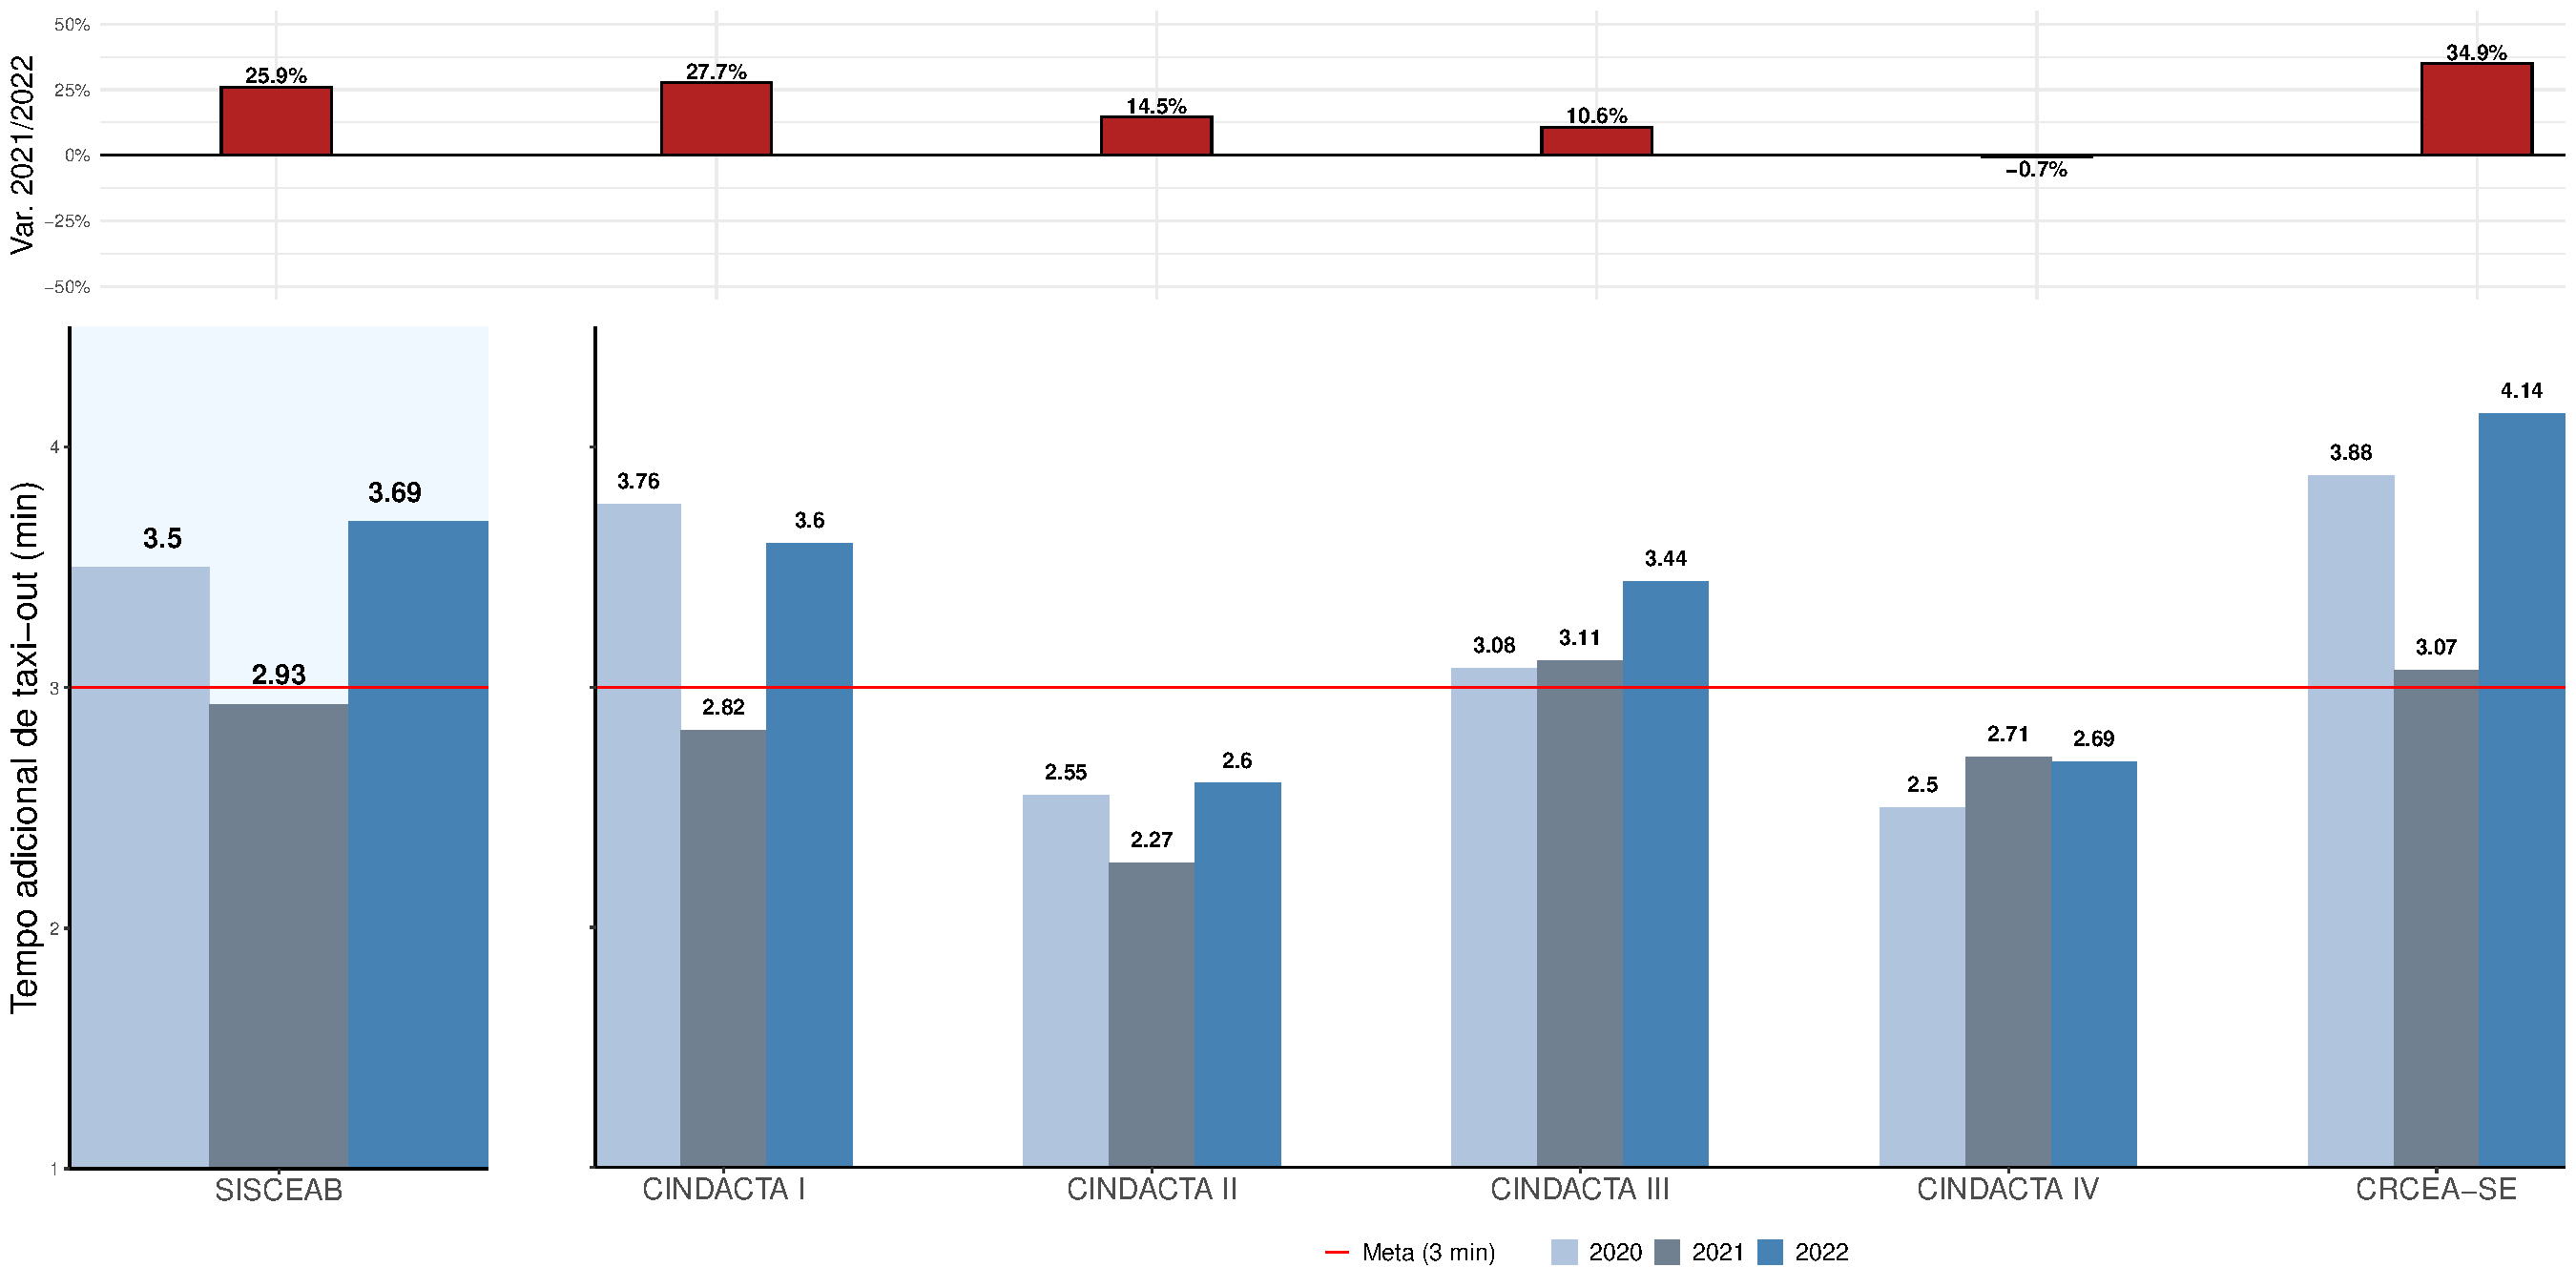
\includegraphics{_main_files/figure-latex/unnamed-chunk-27-2.pdf}

\#18 TAXI-IN 2022

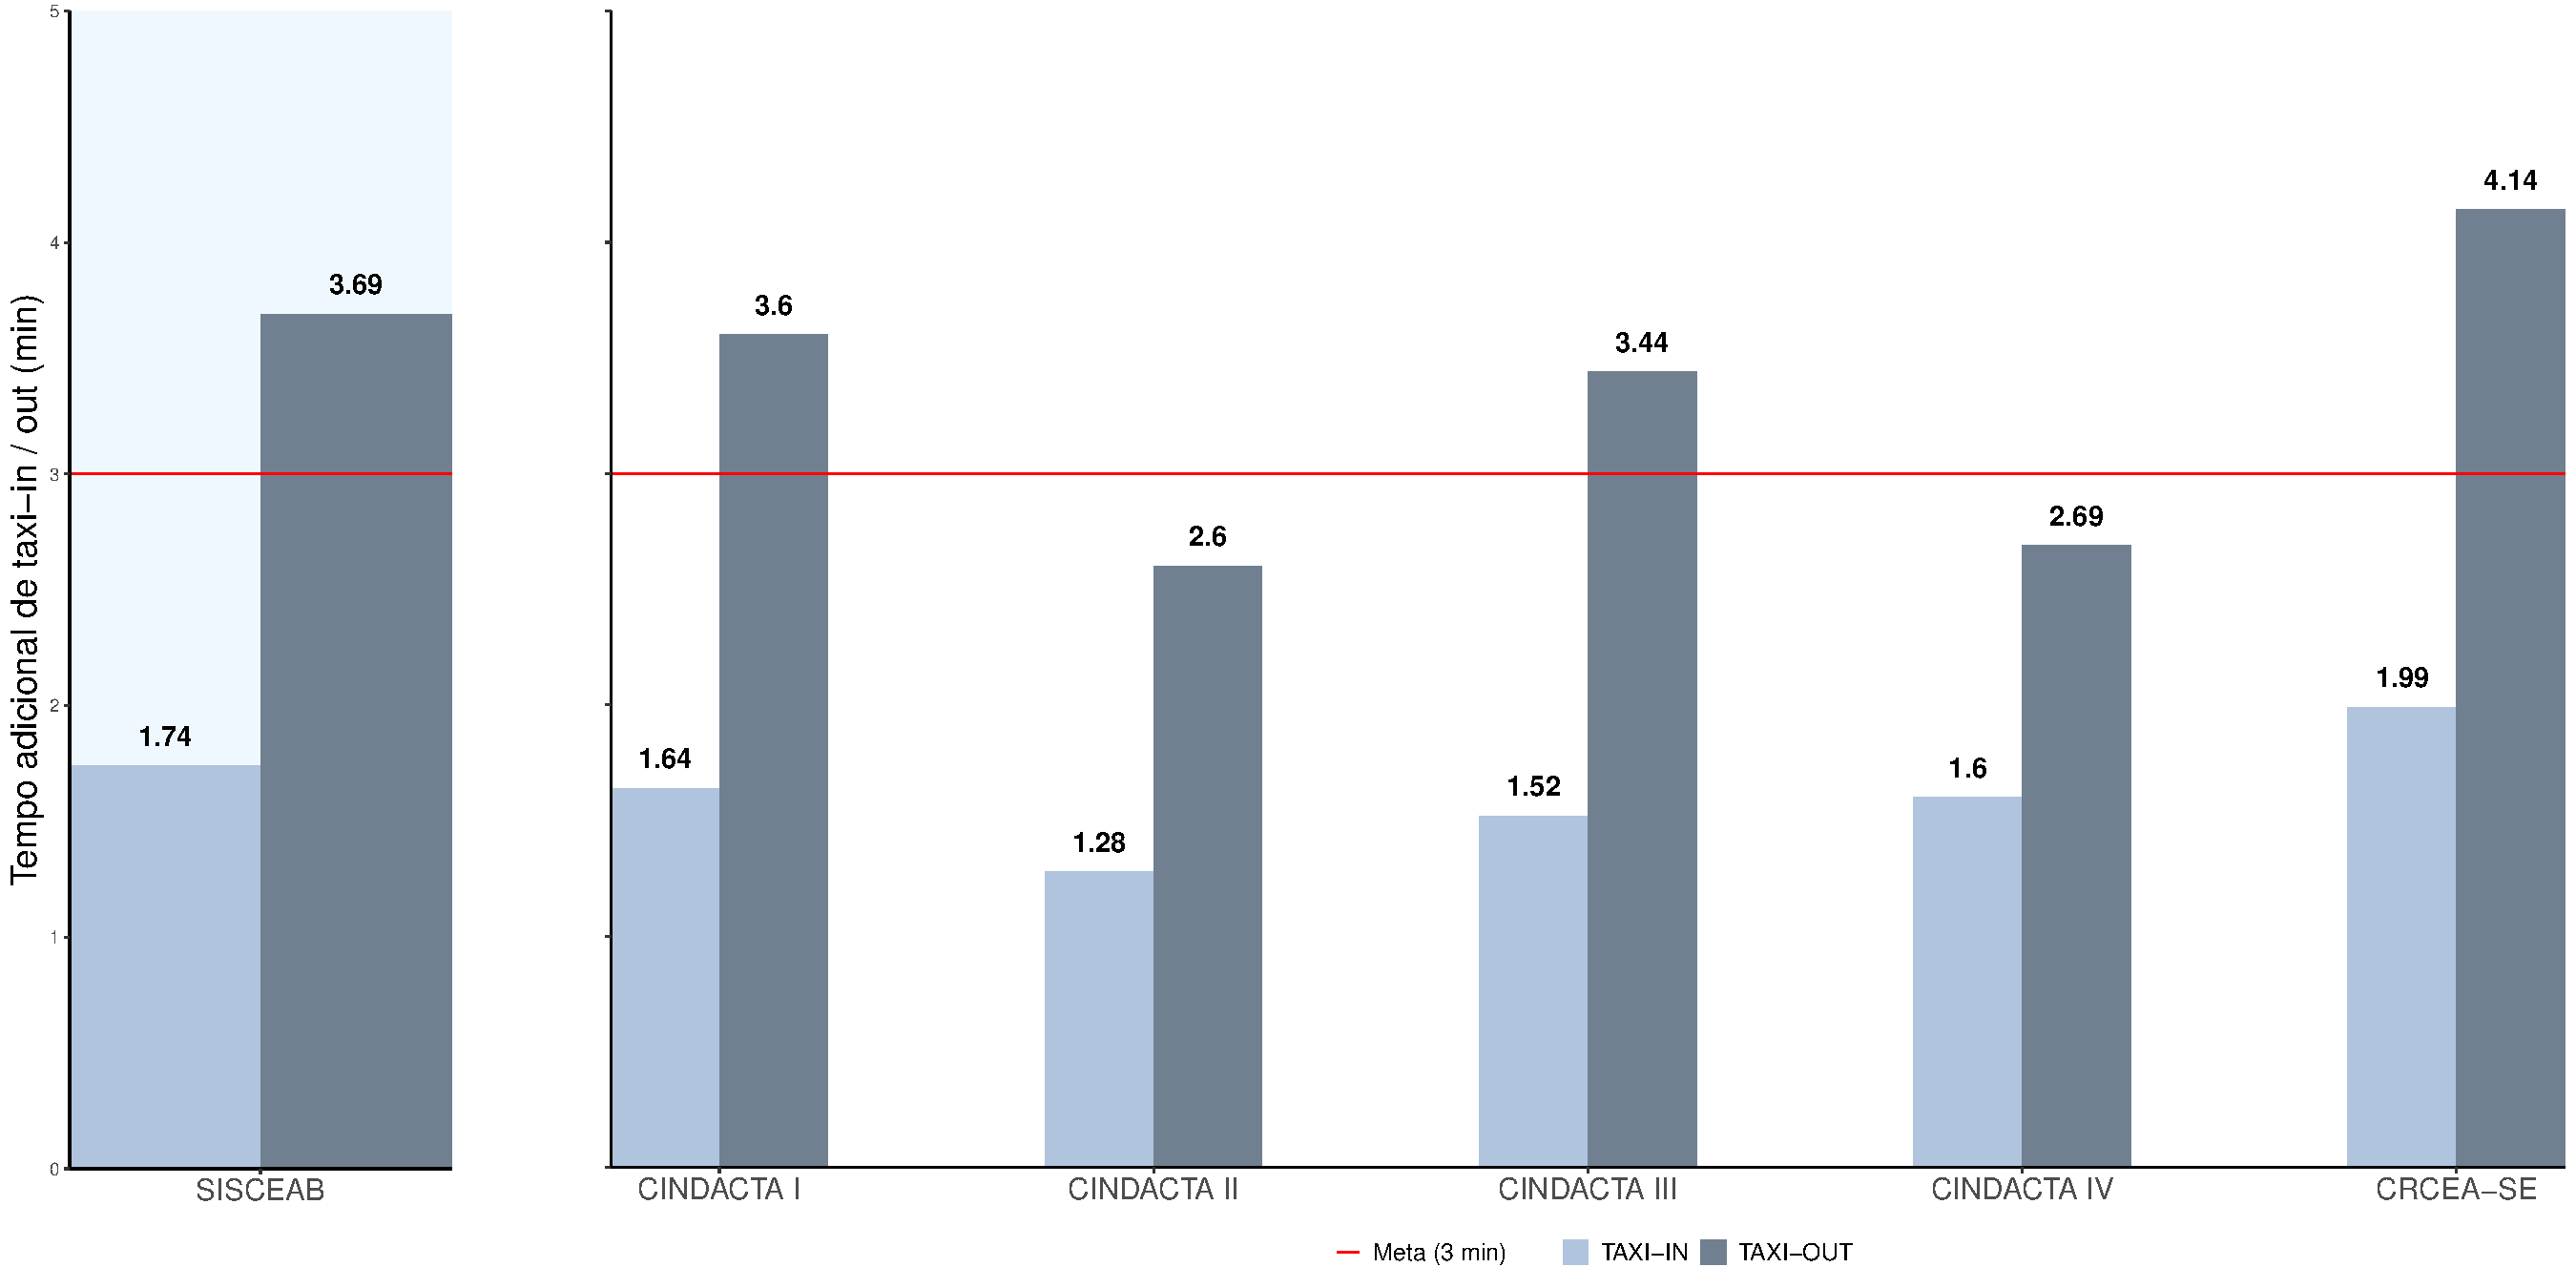
\includegraphics{_main_files/figure-latex/unnamed-chunk-28-1.pdf}

\#19 GRÁFICO DE TEMPO ADICIONAL DE TAXI-IN POR REGIONAL

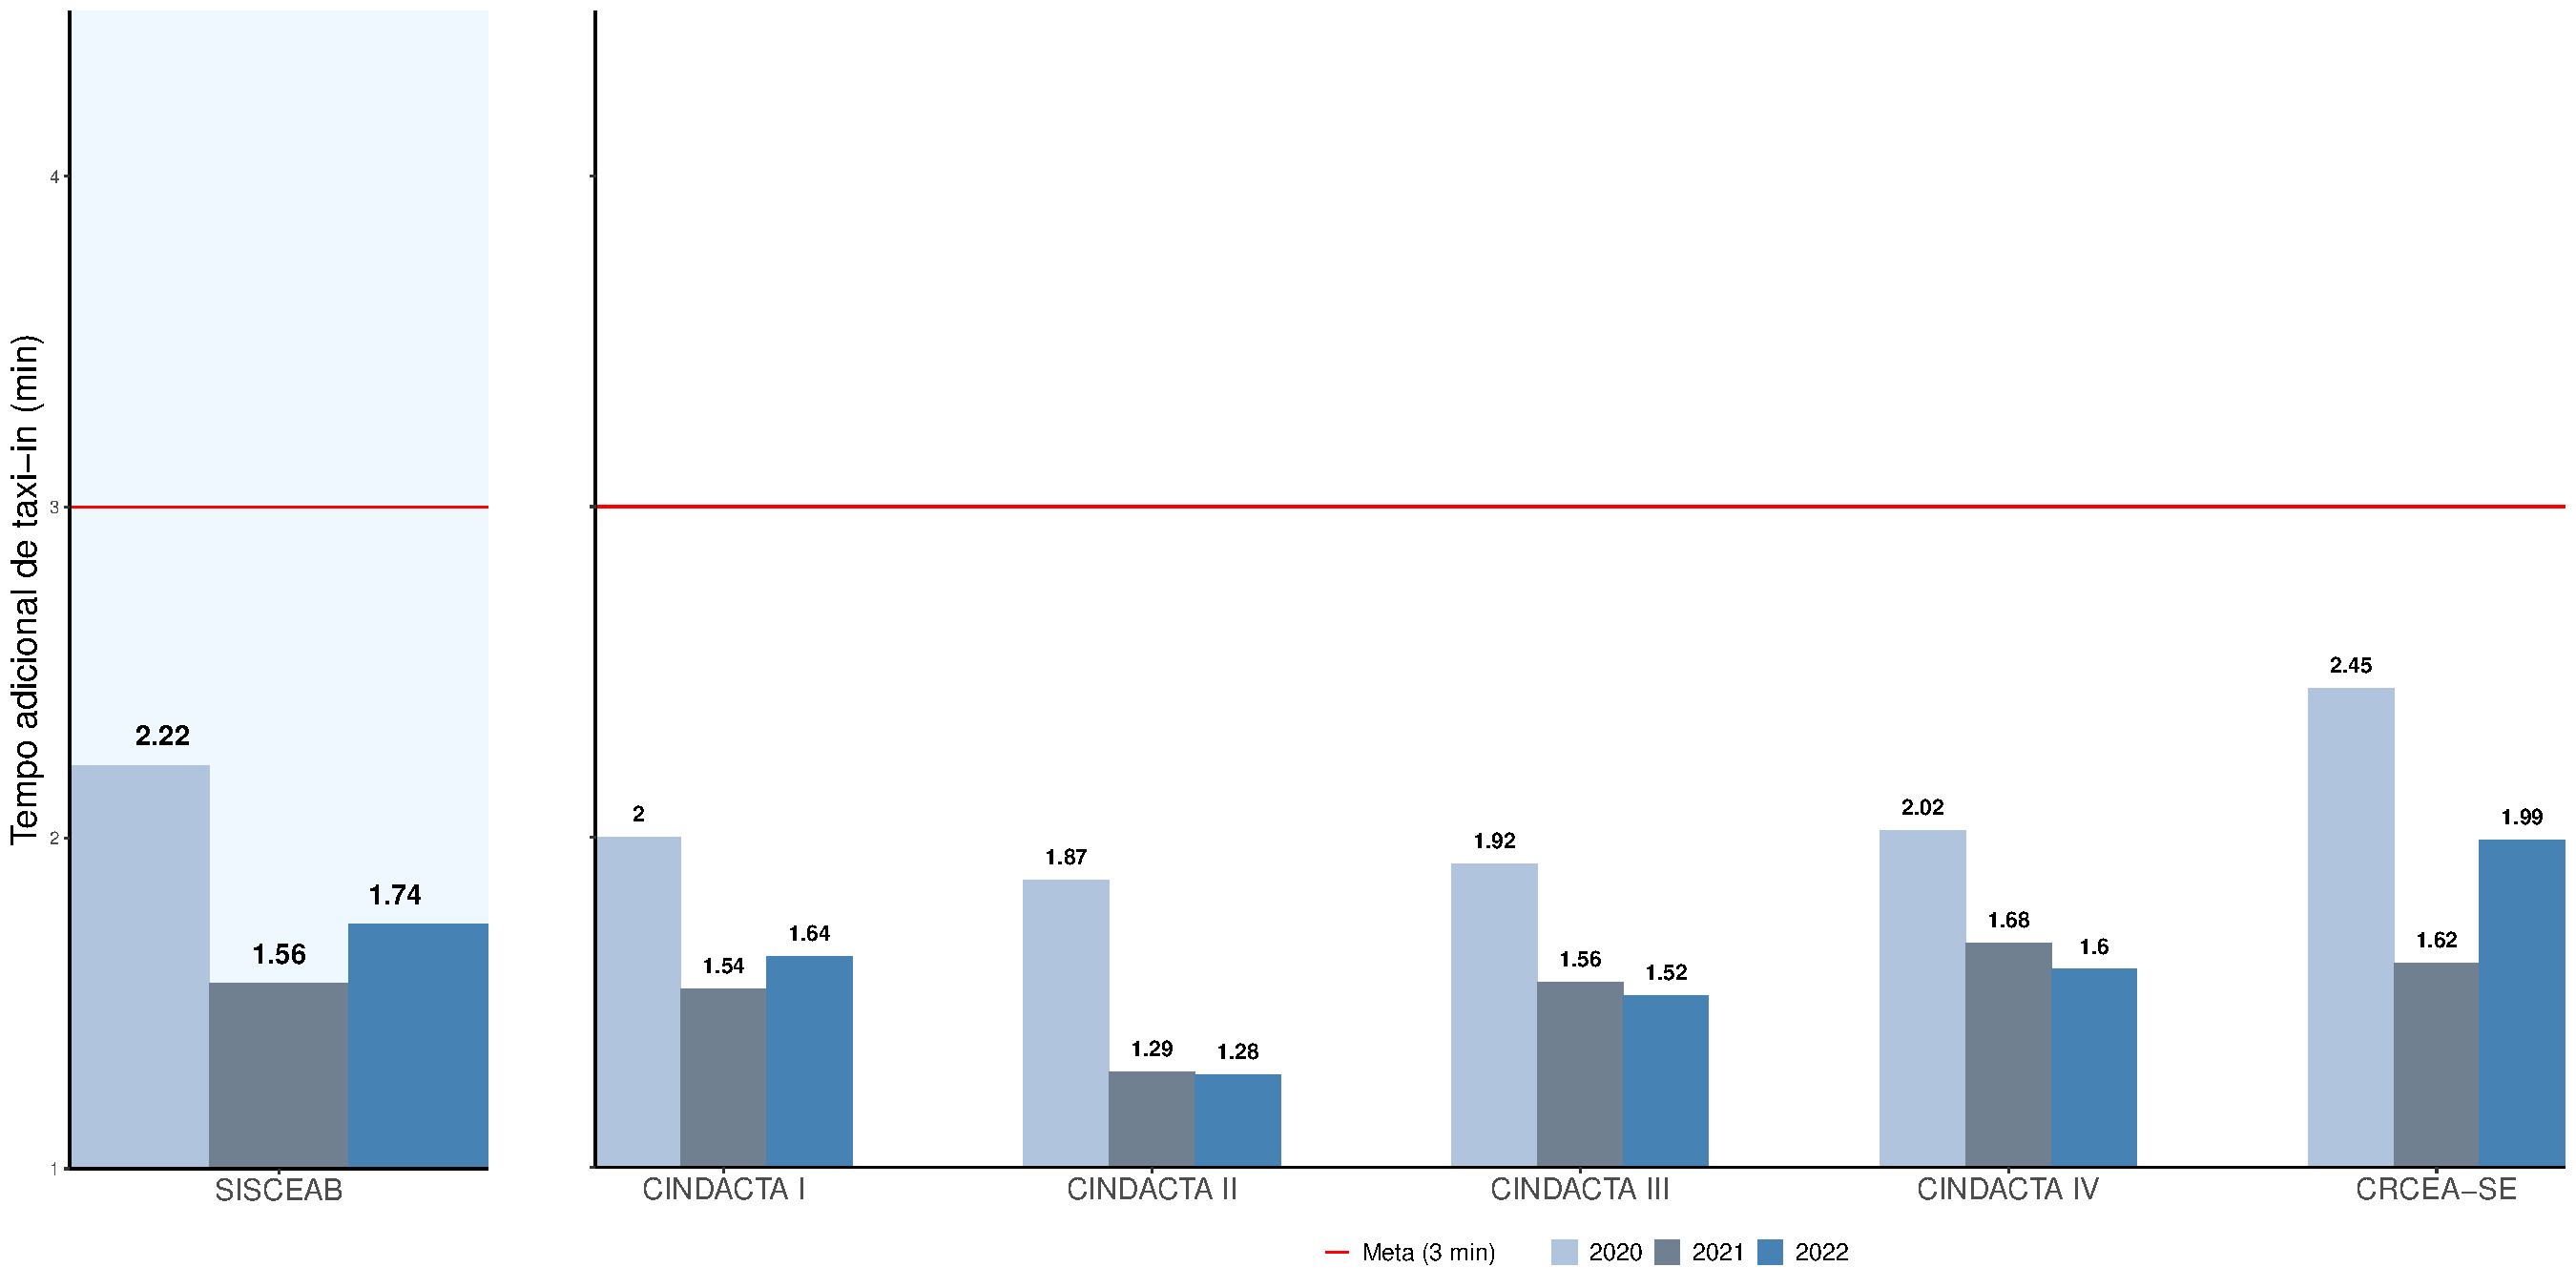
\includegraphics{_main_files/figure-latex/unnamed-chunk-29-1.pdf} 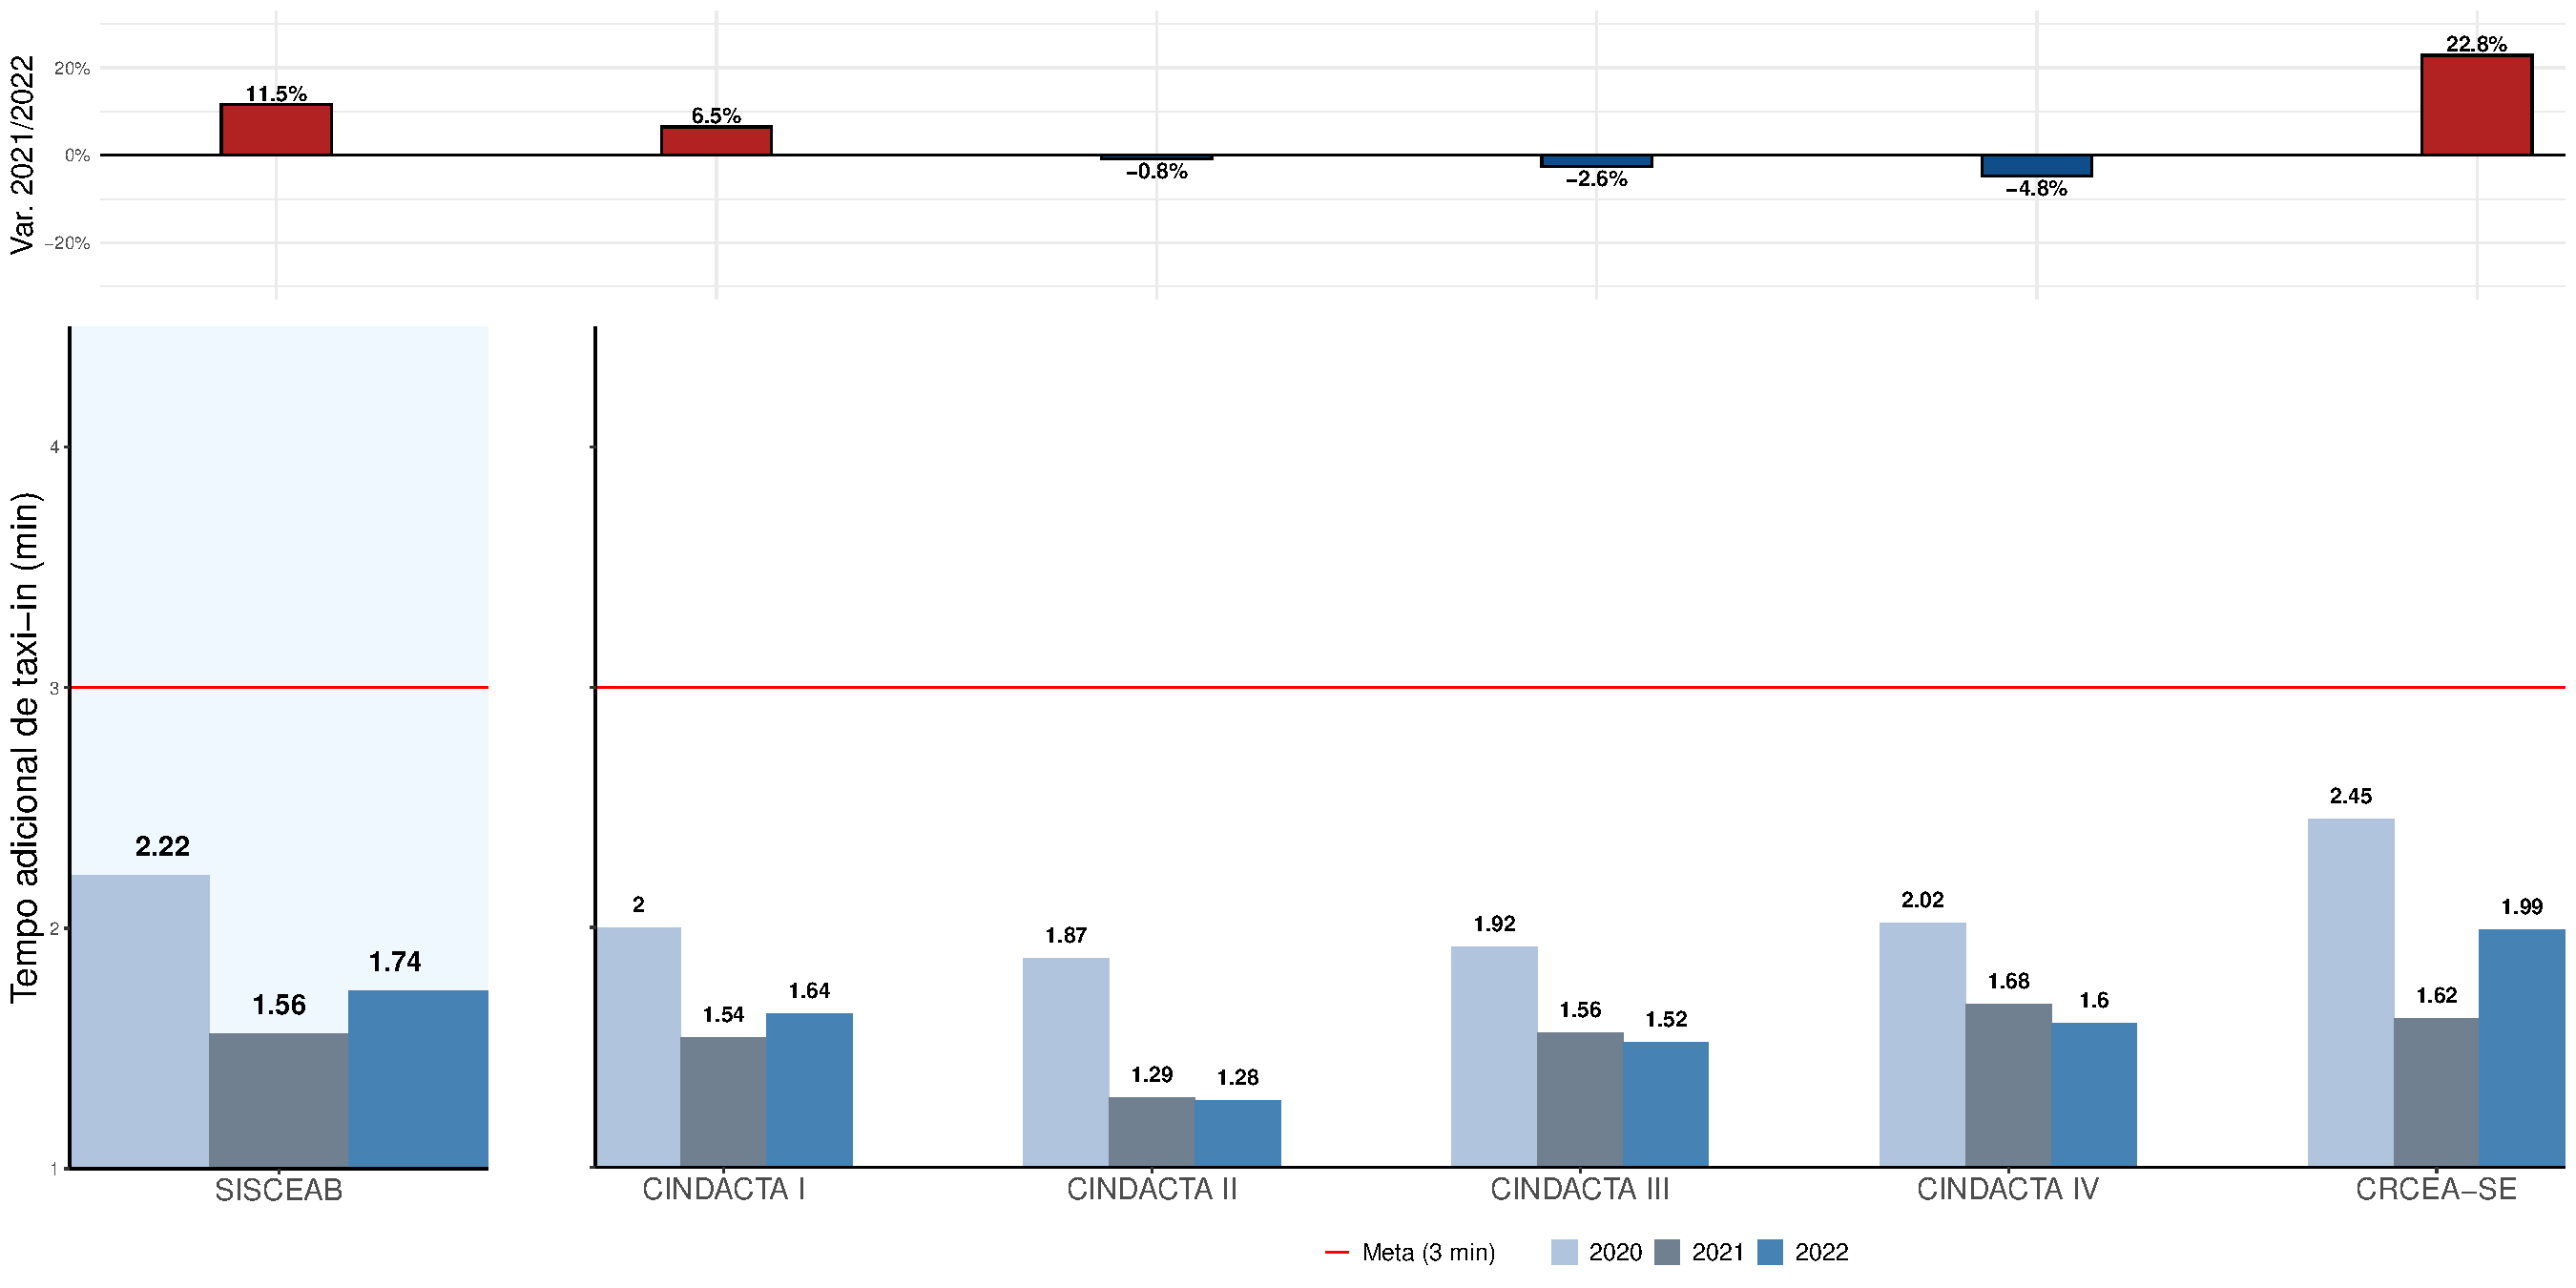
\includegraphics{_main_files/figure-latex/unnamed-chunk-29-2.pdf}

\#20 GRÁFICO DE TEMPO ADICIONAL DE TAXI-IN/OUT POR AEROPORTO

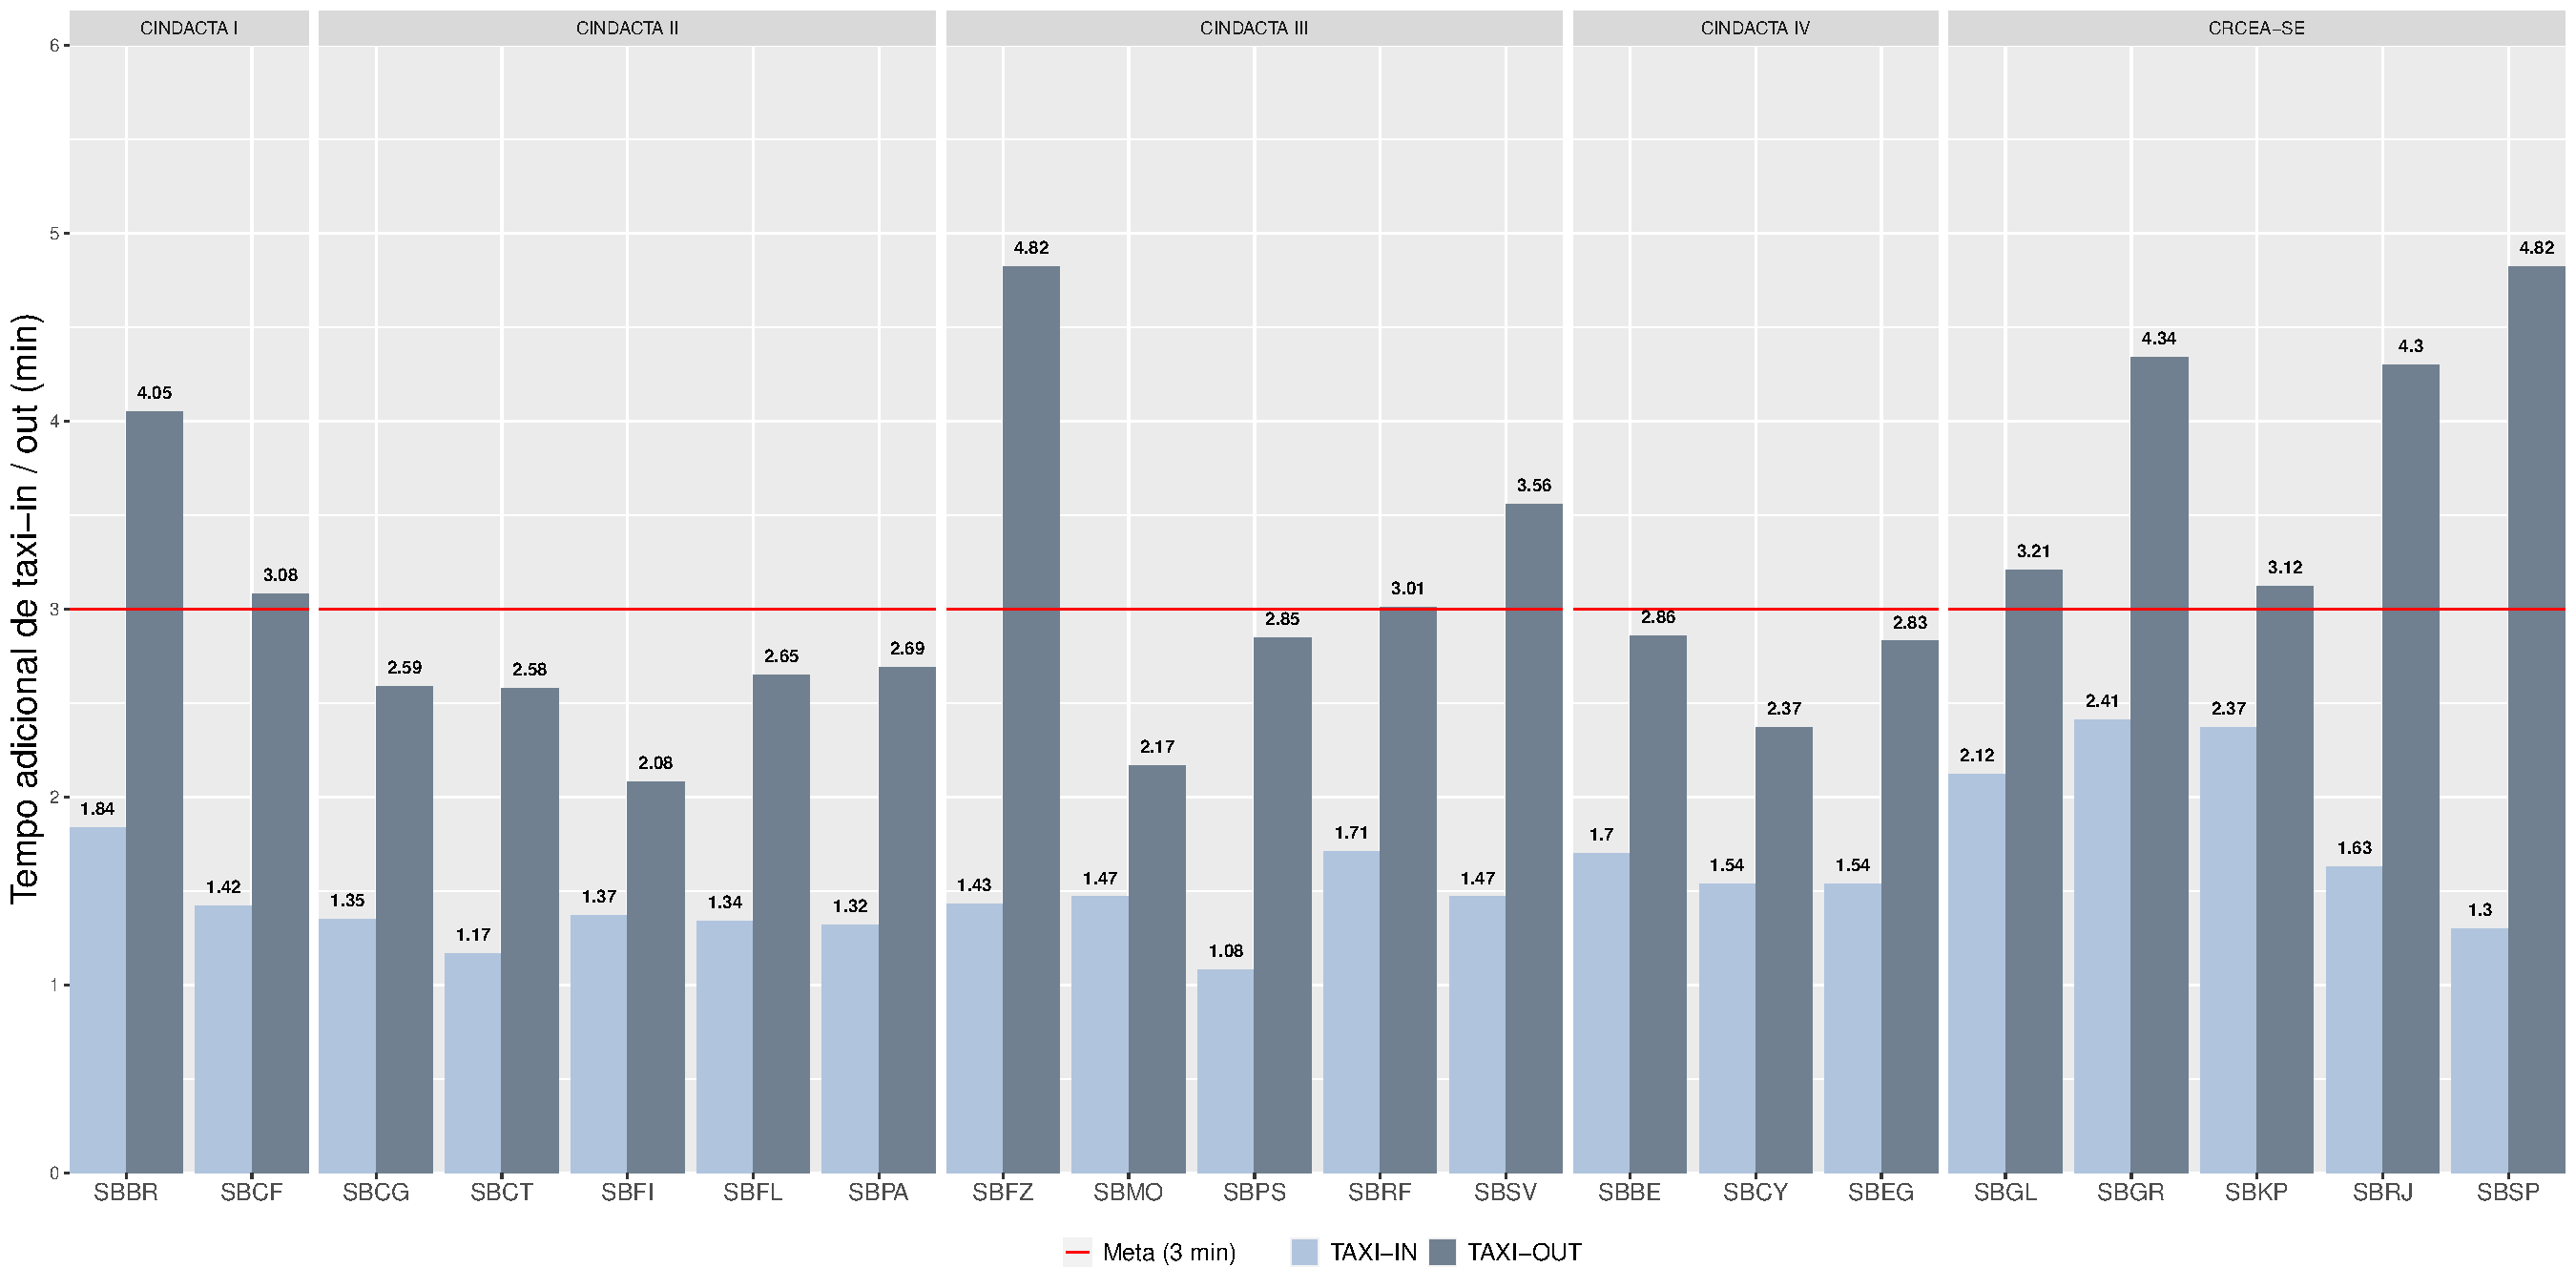
\includegraphics{_main_files/figure-latex/unnamed-chunk-30-1.pdf}

\#\#20.1 GRÁFICO DE TEMPO ADICIONAL DE TAXI-IN/OUT POR REGIONAL

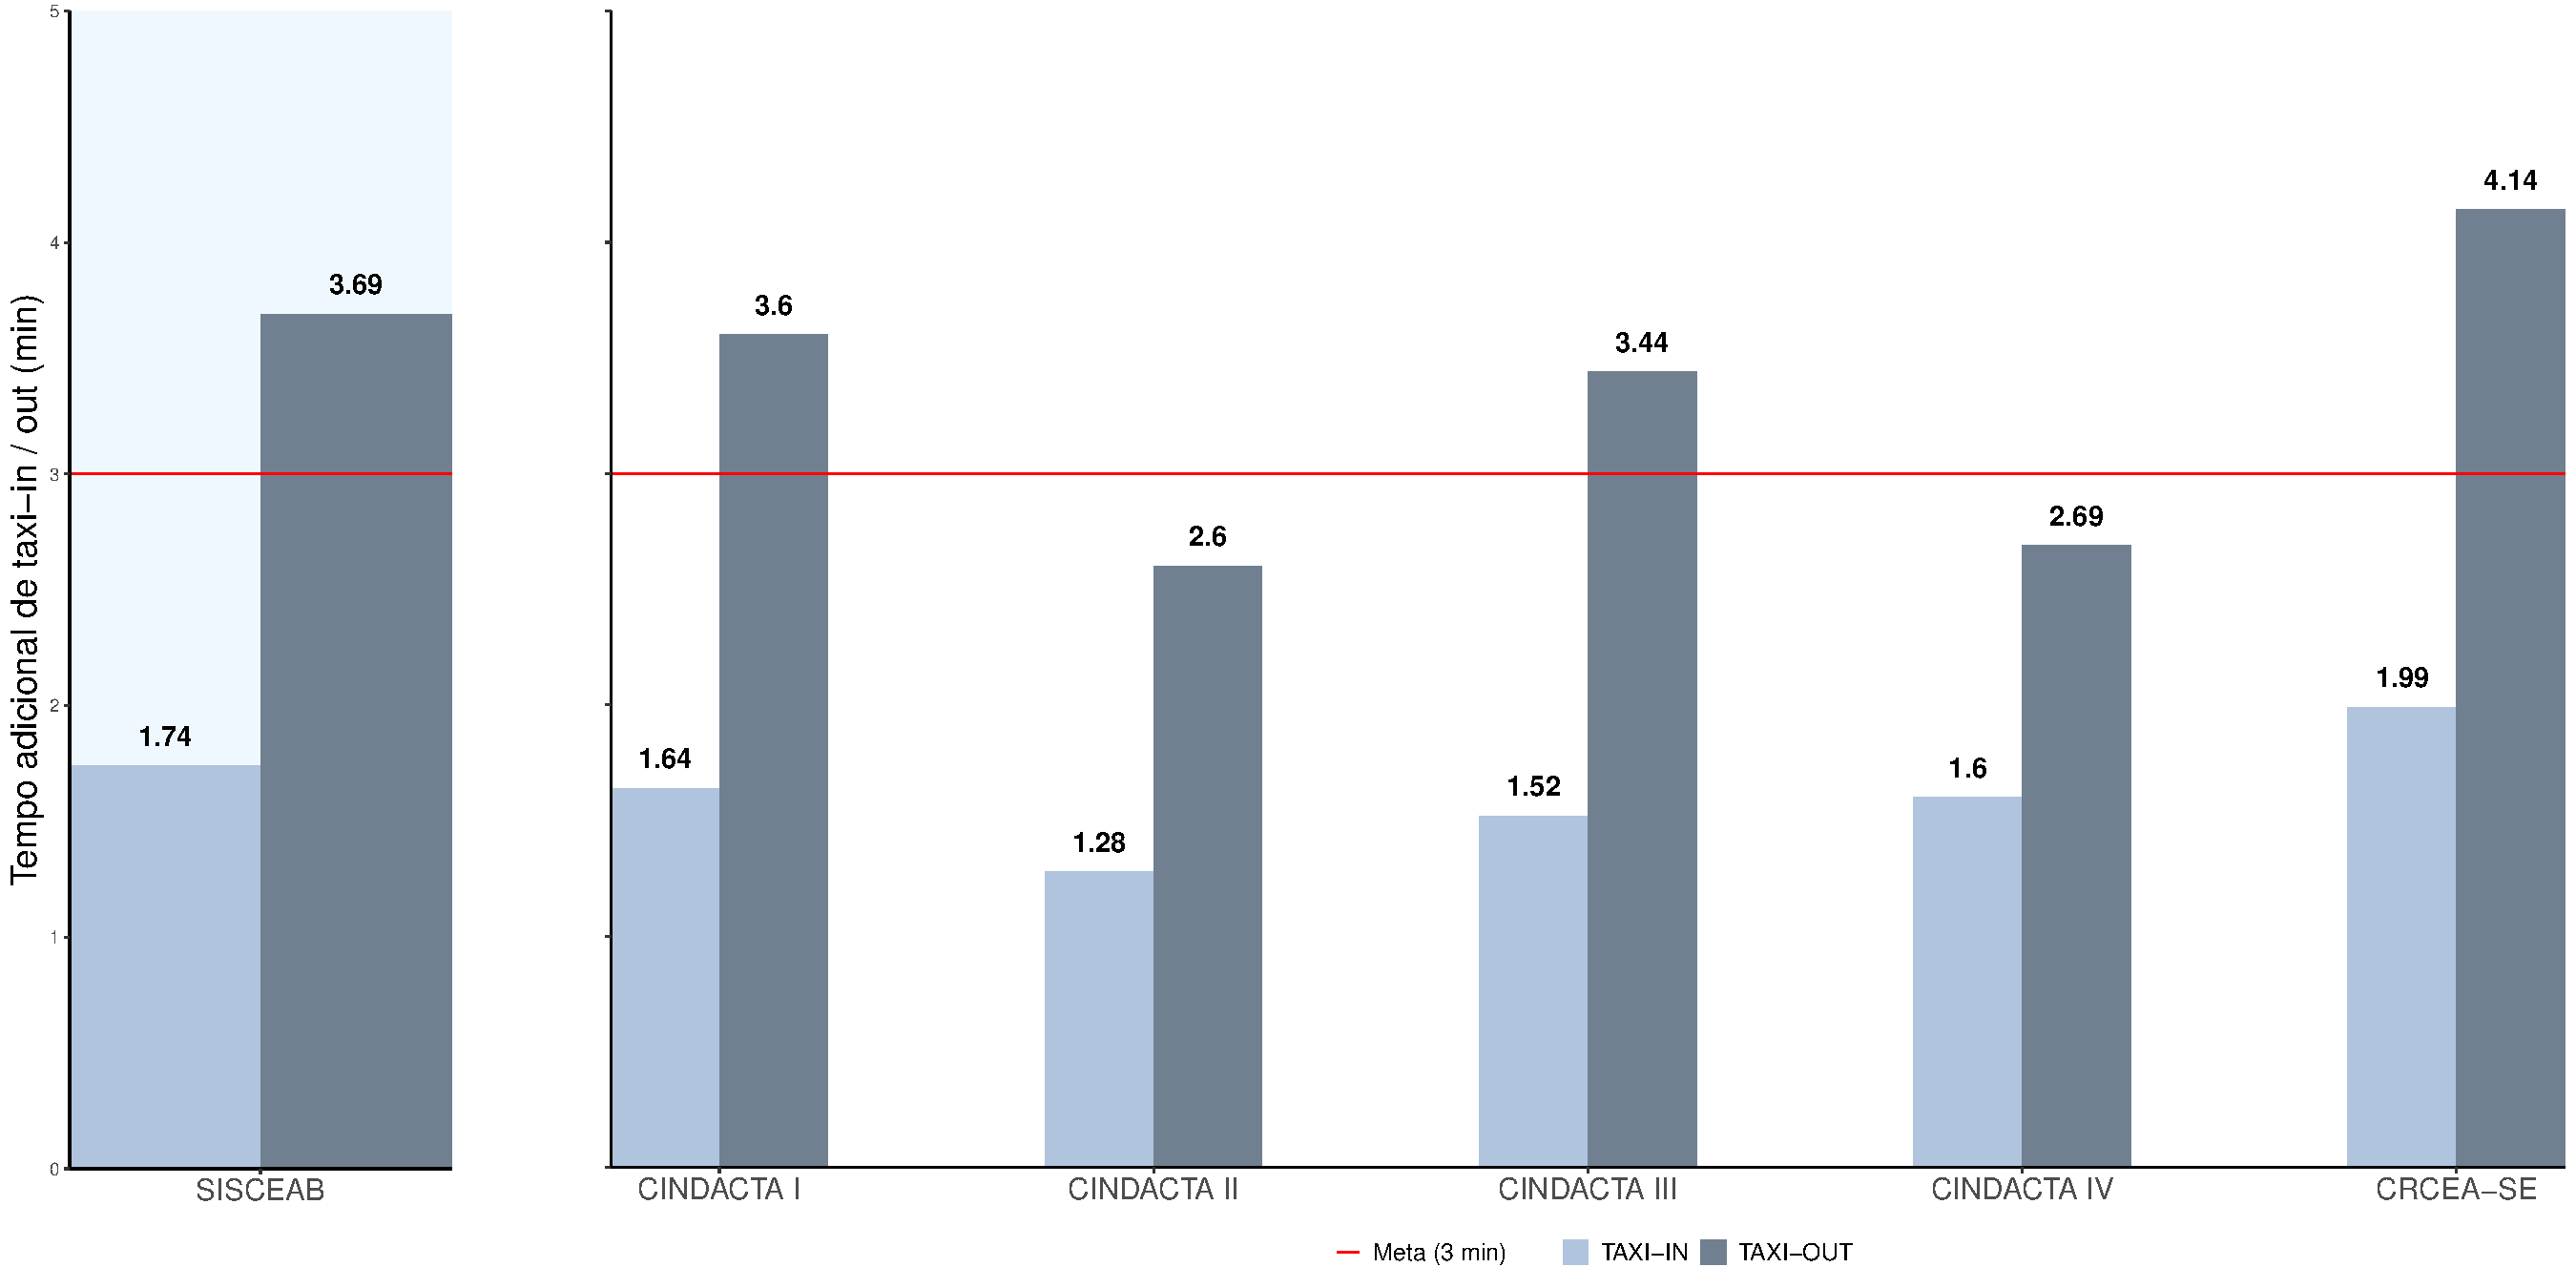
\includegraphics{_main_files/figure-latex/unnamed-chunk-31-1.pdf}

\#21 Rotas mais voadas em 2022

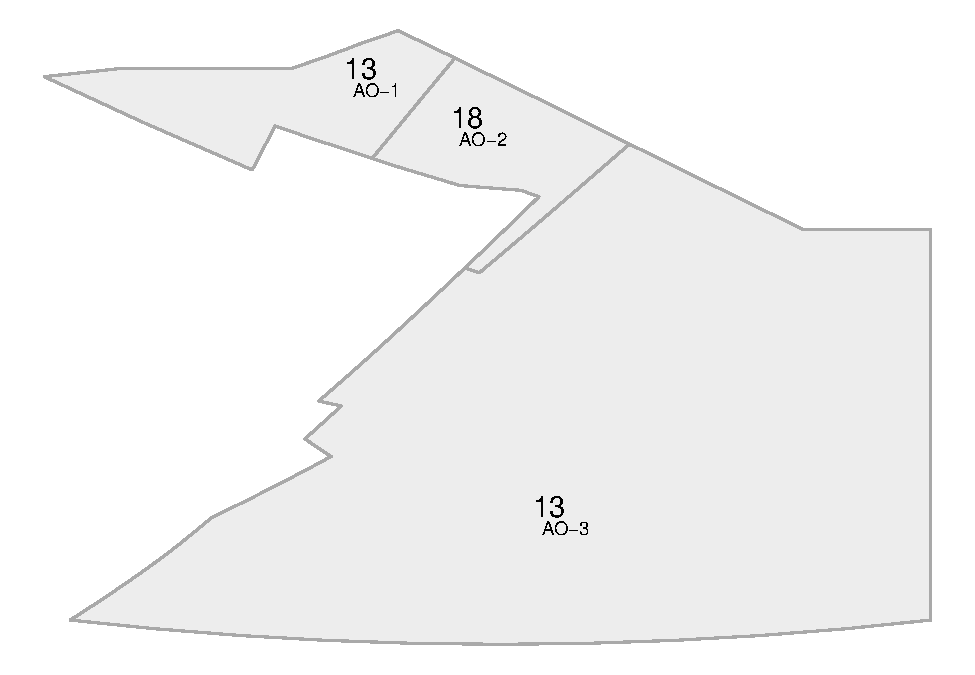
\includegraphics{_main_files/figure-latex/unnamed-chunk-32-1.pdf}

\#TEMPO ADICIONAL EM TMA

\#\#22.1 TEMPO ADICIONAL EM TMA

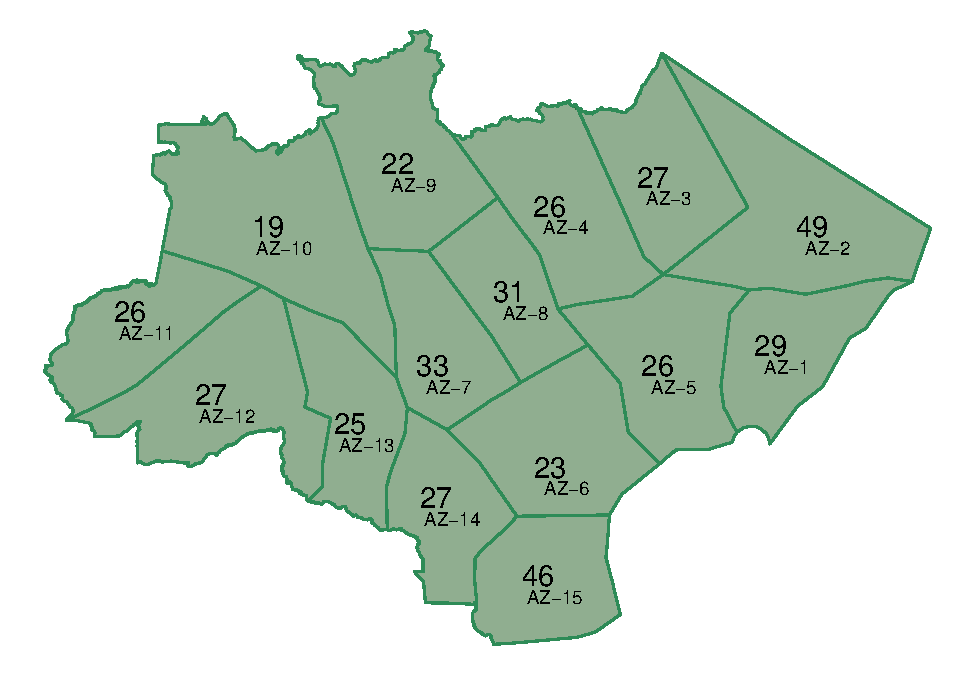
\includegraphics{_main_files/figure-latex/unnamed-chunk-33-1.pdf}

\#\#22.2 TEMPO ADICIONAL EM TMA SBGR

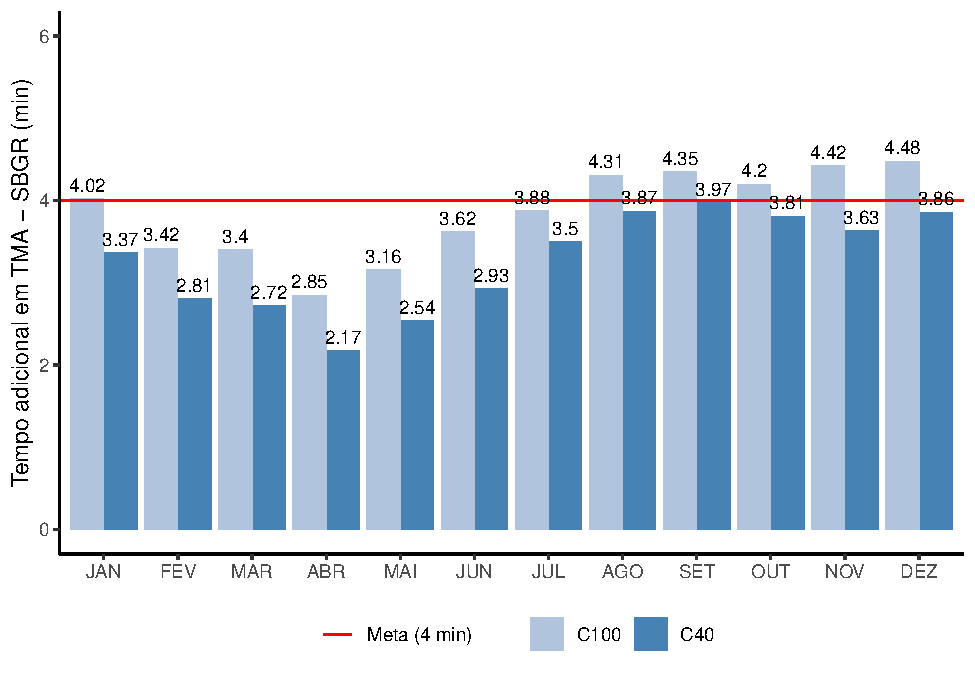
\includegraphics{_main_files/figure-latex/unnamed-chunk-34-1.pdf}

\#\#22.3 TEMPO ADICIONAL EM TMA SBSP

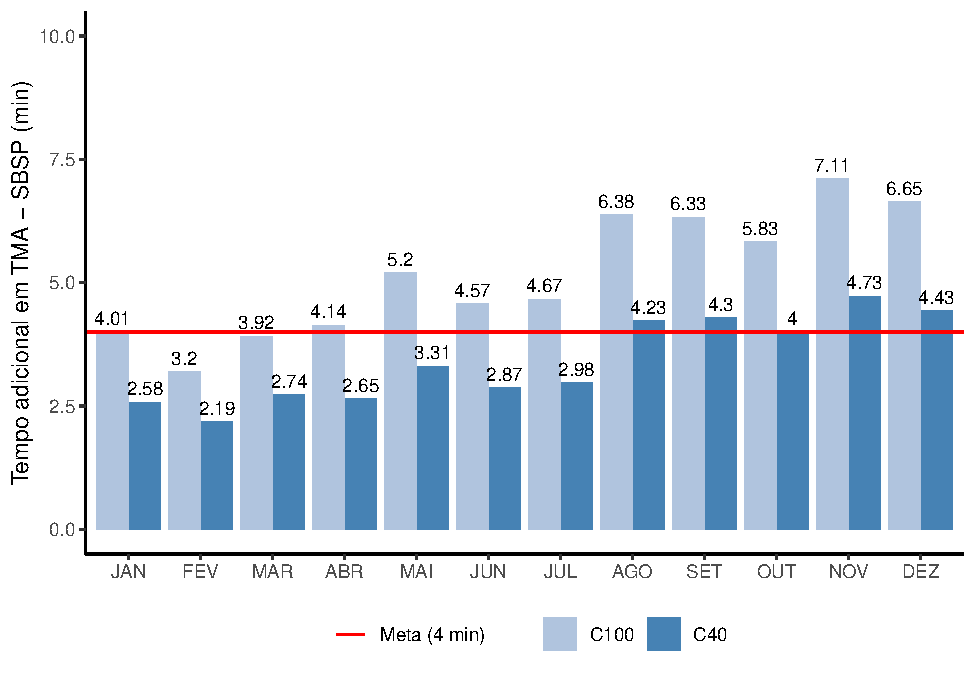
\includegraphics{_main_files/figure-latex/unnamed-chunk-35-1.pdf}

\#\#22.4 TEMPO ADICIONAL EM TMA SBCF

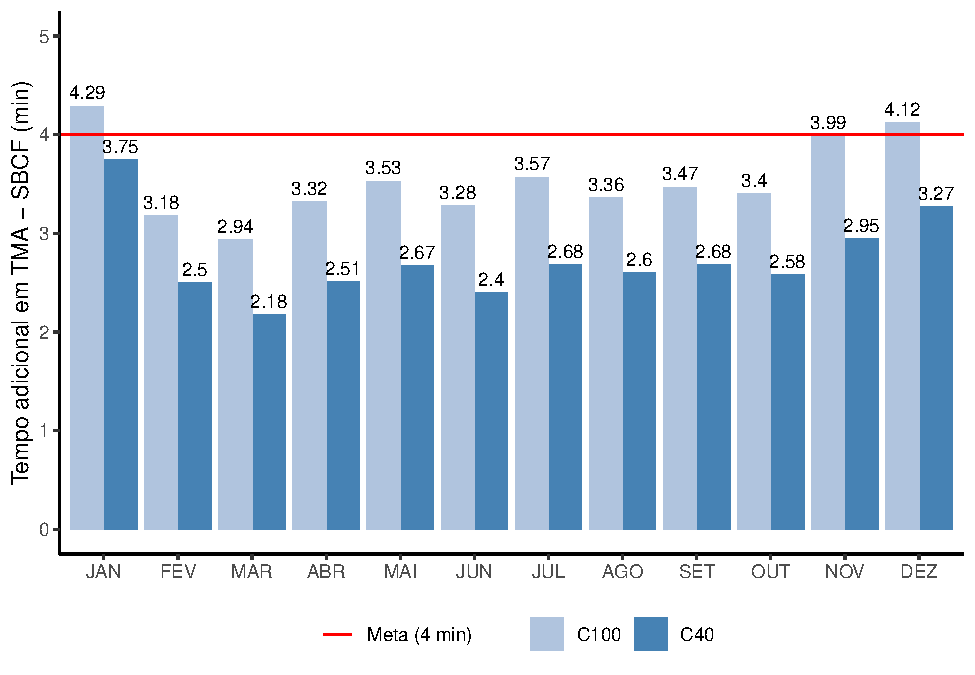
\includegraphics{_main_files/figure-latex/unnamed-chunk-36-1.pdf}

\#\#22.5 TEMPO ADICIONAL EM TMA REGIONAL

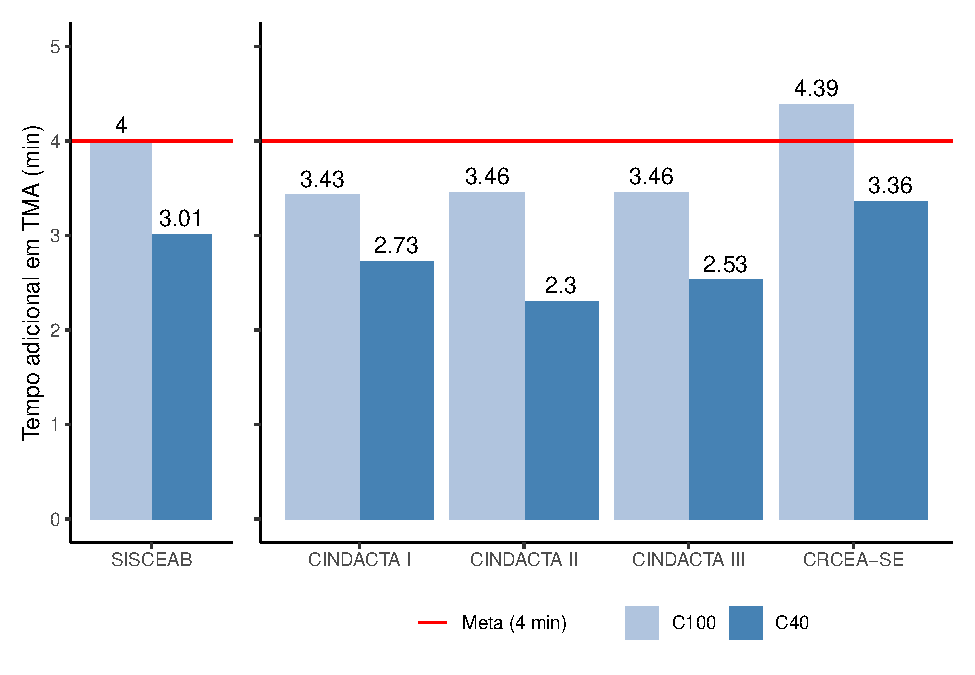
\includegraphics{_main_files/figure-latex/unnamed-chunk-37-1.pdf}
\#\# 22.6 TEMPO ADICIONAL EM TMA C40 COM VAR

\includegraphics{_main_files/figure-latex/unnamed-chunk-38-1.pdf}

\hypertarget{tempo-adicional-em-tma-c100-com-var}{%
\section{22.7 TEMPO ADICIONAL EM TMA C100 COM VAR}\label{tempo-adicional-em-tma-c100-com-var}}

\includegraphics{_main_files/figure-latex/unnamed-chunk-39-1.pdf}

\#Horas de LOGIN X horas de escala

\#23.1 Horas de LOGIN X horas de escala ACC

\includegraphics{_main_files/figure-latex/unnamed-chunk-40-1.pdf}

\hypertarget{horas-de-login-x-horas-de-escala-app}{%
\section{23.2 Horas de LOGIN X horas de escala APP}\label{horas-de-login-x-horas-de-escala-app}}

\includegraphics{_main_files/figure-latex/unnamed-chunk-41-1.pdf}

\hypertarget{horas-de-login-x-horas-de-escala-twr}{%
\section{23.3 Horas de LOGIN X horas de escala TWR}\label{horas-de-login-x-horas-de-escala-twr}}

\includegraphics{_main_files/figure-latex/unnamed-chunk-42-1.pdf}

\hypertarget{mapas-chs}{%
\chapter{MAPAS CHS}\label{mapas-chs}}

\hypertarget{mapa-setor-sbbs}{%
\section{24.1 MAPA SETOR SBBS}\label{mapa-setor-sbbs}}

\includegraphics{_main_files/figure-latex/unnamed-chunk-43-1.pdf}

\#\#24.2 MAPA SETOR SBCW

\includegraphics{_main_files/figure-latex/unnamed-chunk-44-1.pdf}

\hypertarget{mapa-setor-sbre}{%
\section{24.3 MAPA SETOR SBRE}\label{mapa-setor-sbre}}

\includegraphics{_main_files/figure-latex/unnamed-chunk-45-1.pdf}

\hypertarget{mapa-setor-sbaz}{%
\section{24.4 MAPA SETOR SBAZ}\label{mapa-setor-sbaz}}

\includegraphics{_main_files/figure-latex/unnamed-chunk-46-1.pdf}

\#\#24.5 MAPA SETOR SBAO

\includegraphics{_main_files/figure-latex/unnamed-chunk-47-1.pdf}

\hypertarget{mapas-de-fir}{%
\chapter{MAPAS de FIR}\label{mapas-de-fir}}

\hypertarget{mapa-setor-sbbs-1}{%
\section{25.1 MAPA SETOR SBBS}\label{mapa-setor-sbbs-1}}

\includegraphics{_main_files/figure-latex/unnamed-chunk-48-1.pdf}

\#\#25.2 MAPA SETOR SBCW

\includegraphics{_main_files/figure-latex/unnamed-chunk-49-1.pdf}

\hypertarget{mapa-setor-sbre-1}{%
\section{25.3 MAPA SETOR SBRE}\label{mapa-setor-sbre-1}}

\includegraphics{_main_files/figure-latex/unnamed-chunk-50-1.pdf}

\hypertarget{mapa-setor-sbaz-1}{%
\section{25.4 MAPA SETOR SBAZ}\label{mapa-setor-sbaz-1}}

\includegraphics{_main_files/figure-latex/unnamed-chunk-51-1.pdf}

\#\#25.5 MAPA SETOR SBAO

\includegraphics{_main_files/figure-latex/unnamed-chunk-52-1.pdf}

\end{document}
